\documentclass[a4paper]{report}
\usepackage[margin=3.5cm]{geometry}
\usepackage[pdftex]{hyperref}
\usepackage[svgnames]{xcolor}
\usepackage{amsmath,amsfonts,amssymb,amsthm,thmtools,thm-restate}
\usepackage{bookmark,graphicx,dsfont,datetime,float,booktabs,enumitem,outlines,nicematrix}
\usepackage{tabularx,ragged2e,adjustbox} % for literature table
\usepackage{tocloft}    % customize toc entries
\usepackage{xpatch}     % for bookmark 'hack' for appendix naming
\usepackage{setspace}   % for bookmark fix of bibliography

\usepackage{pdfcomment} % adding floating pdf comments
\newcommand{\comment}[1]{\pdfmargincomment[author=Jeroen van Riel]{#1}}

% micro-level typesetting
\usepackage[activate={true,nocompatibility},final,tracking=true,kerning=true,spacing=true,
            factor=500,stretch=15,shrink=15]{microtype}

% theorem environments
\theoremstyle{definition}
\newtheorem{eg}{Example}[chapter]
\newtheorem{define}{Definition}[chapter]
\theoremstyle{plain}
\newtheorem{proposition}{Proposition}[chapter]
\newtheorem{lemma}{Lemma}[chapter]
\newtheorem{theorem}{Theorem}[chapter]
\newtheorem{assump}{Assumption}[chapter]
\newtheorem{remark}{Remark}[chapter]

% load styling for knitr produced tables
\definecolor{fgcolor}{rgb}{0.345, 0.345, 0.345}
\newcommand{\hlnum}[1]{\textcolor[rgb]{0.686,0.059,0.569}{#1}}%
\newcommand{\hlstr}[1]{\textcolor[rgb]{0.192,0.494,0.8}{#1}}%
\newcommand{\hlcom}[1]{\textcolor[rgb]{0.678,0.584,0.686}{\textit{#1}}}%
\newcommand{\hlopt}[1]{\textcolor[rgb]{0,0,0}{#1}}%
\newcommand{\hlstd}[1]{\textcolor[rgb]{0.345,0.345,0.345}{#1}}%
\newcommand{\hlkwa}[1]{\textcolor[rgb]{0.161,0.373,0.58}{\textbf{#1}}}%
\newcommand{\hlkwb}[1]{\textcolor[rgb]{0.69,0.353,0.396}{#1}}%
\newcommand{\hlkwc}[1]{\textcolor[rgb]{0.333,0.667,0.333}{#1}}%
\newcommand{\hlkwd}[1]{\textcolor[rgb]{0.737,0.353,0.396}{\textbf{#1}}}%
\let\hlipl\hlkwb

\usepackage{framed}
\makeatletter
\newenvironment{kframe}{%
 \def\at@end@of@kframe{}%
 \ifinner\ifhmode%
  \def\at@end@of@kframe{\end{minipage}}%
  \begin{minipage}{\columnwidth}%
 \fi\fi%
 \def\FrameCommand##1{\hskip\@totalleftmargin \hskip-\fboxsep
 \colorbox{shadecolor}{##1}\hskip-\fboxsep
     % There is no \\@totalrightmargin, so:
     \hskip-\linewidth \hskip-\@totalleftmargin \hskip\columnwidth}%
 \MakeFramed {\advance\hsize-\width
   \@totalleftmargin\z@ \linewidth\hsize
   \@setminipage}}%
 {\par\unskip\endMakeFramed%
 \at@end@of@kframe}
\makeatother

\definecolor{shadecolor}{rgb}{.97, .97, .97}
\definecolor{messagecolor}{rgb}{0, 0, 0}
\definecolor{warningcolor}{rgb}{1, 0, 1}
\definecolor{errorcolor}{rgb}{1, 0, 0}
\newenvironment{knitrout}{}{} % an empty environment to be redefined in TeX


\DeclareMathOperator{\interior}{int}
\DeclareMathOperator*{\argmax}{arg\,max}
\DeclareMathOperator*{\argmin}{arg\,min}
\newcommand\halfopen[2]{\ensuremath{[#1,#2)}}
\newcommand\openhalf[2]{\ensuremath{(#1,#2]}}
\newcommand*\diff{\mathop{}\!\mathrm{d}}

\newcommand\note[1]{{\color{Navy}#1}}

% set title, date and author
\newdateformat{monthyeardate}{\monthname[\THEMONTH] \THEYEAR}
\author{Jeroen van Riel}
\date{\monthyeardate\today}
\newcommand{\mytitle}{\huge Machine Learning-Based Scheduling for the Coordination of Automated Vehicles}
\title{\mytitle}

% set pdf meta-data
\hypersetup{
    pdftitle = {\mytitle},
    pdfauthor = {Jeroen van Riel}
}

\begin{document}

%
% title page with abstract
%
\noindent\makebox[\textwidth][c]{%
\begin{minipage}[h]{\textwidth}
    \maketitle
    \begin{center}
    \textbf{Abstract}
    \end{center}
    Coordination of automated vehicles in a network of intersections is modeled
    as a trajectory optimization problem. Under certain model assumptions, this
    problem can be decomposed into (i) an upper-level scheduling problem of
    determining the crossing times at intersections and (ii) a set of
    lower-level trajectory optimization problems. We show that the feasibility
    of the lower-level problems is characterized as a set of linear inequalities
    in the crossing times.
    %
    Since schedules can be interpreted as a sequence of discrete decisison, we
    experiment with sequence modeling to solve the crossing time scheduling. We
    compare a simple parameterization with a neural network model. As previously
    observed by others, our case study illustrates that the evaluation order of
    the sequence model matters for the final performance.
\end{minipage}}

% \begin{figure}[b!]
%   \centering
%   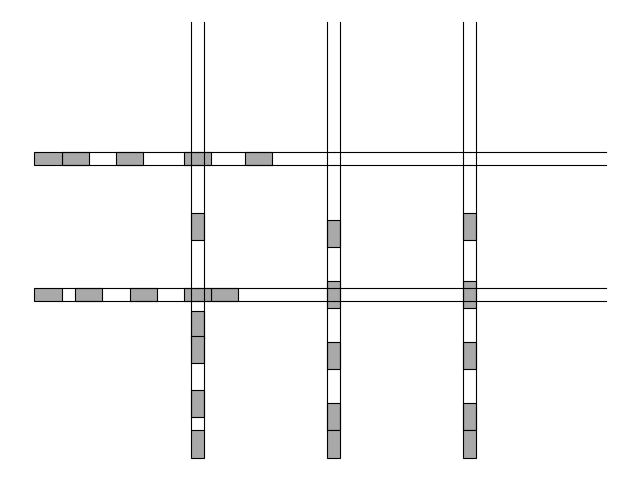
\includegraphics[width=0.7\textwidth]{figures/network/grid_example.png}
% \end{figure}

%
% table of contents setup
%

% 'parts' in toc without page numbers
% the 'Part' text is included manually
\cftpagenumbersoff{part}
\renewcommand{\cftpartfont}{\color{red!70!black}}
\renewcommand{\cftpartpresnum}{}

% exclude part level in pdf bookmarks
\makeatletter
\renewcommand{\toclevel@part}{100}
\makeatother

% numbers before each chapter/section in pdf bookmarks
\bookmarksetup{
  numbered,
}

\newpage
\tableofcontents

% add toc entry in pdf bookmarks
\addtocontents{toc}{\protect{\pdfbookmark[0]{\contentsname}{toc}}}


% \chapter*{Preface}
% \addcontentsline{toc}{chapter}{\protect\numberline{}Preface}


% All hand-drawn figures in this thesis were produced by the Ipe extensible
% drawing editor\footnote{\url{https://ipe.otfried.org}}.


\chapter{Introduction and background}

\section{Introduction}

% motivation
% automated vehicles

Given the ongoing advances in self-driving vehicles and wireless communication,
it is very natural to study how these new technologies can be applied to enable
network-wide traffic coordination.
%
Some of the potential benefits of coordinating the motion of groups of automated
vehicles are increased network throughput, reduced energy consumption and better
guarantees on safety in terms of avoiding dangerous situations.

Coordination of automated vehicles with communication has been studied at
various levels of organization~\cite{marianiCoordinationAutonomousVehicles2022}.
A good example of a local coordination methods is platooning of vehicles, where
the aim is to lower energy consumption by reducing aerodynamic resistance. It
has been shown that platooning can also result in a more efficient use of
intersections. On a larger scale, methods like dynamic route optimization have
been proposed to reduce travel delay for all vehicles in the network.
%
The coordination problem has very many aspects that could be modeled and
analyzed. For example, one may think of heterogenous vehicles---in terms of
dynamics or priority---different models of centralized/decentralized
communication between vehicles or with the infrastructure, under different
guarantees on reliability; complex road topology, curved lanes, merging lanes.

However, as we will see, even the most basic models already present fundamental
challenges in ensuring safety and efficiency.
%
Therefore, we will only consider the two most essential elements in this thesis,
being vehicle dynamics and the constraints that are required to model the
allowed paths vehicles may take in order to avoid collisions with the
infrastructure and other vehicles.
%
To keep things simple, we assume that all vehicles are automated and share the
same dynamics.
%
Each vehicle follows a fixed route through the network and is centrally
controlled through acceleration inputs under the assumption of perfect
communication.
%
With these assumptions, the traffic coordination task can be modeled a
trajectory optimization problem.

\begin{figure}
  \centering
  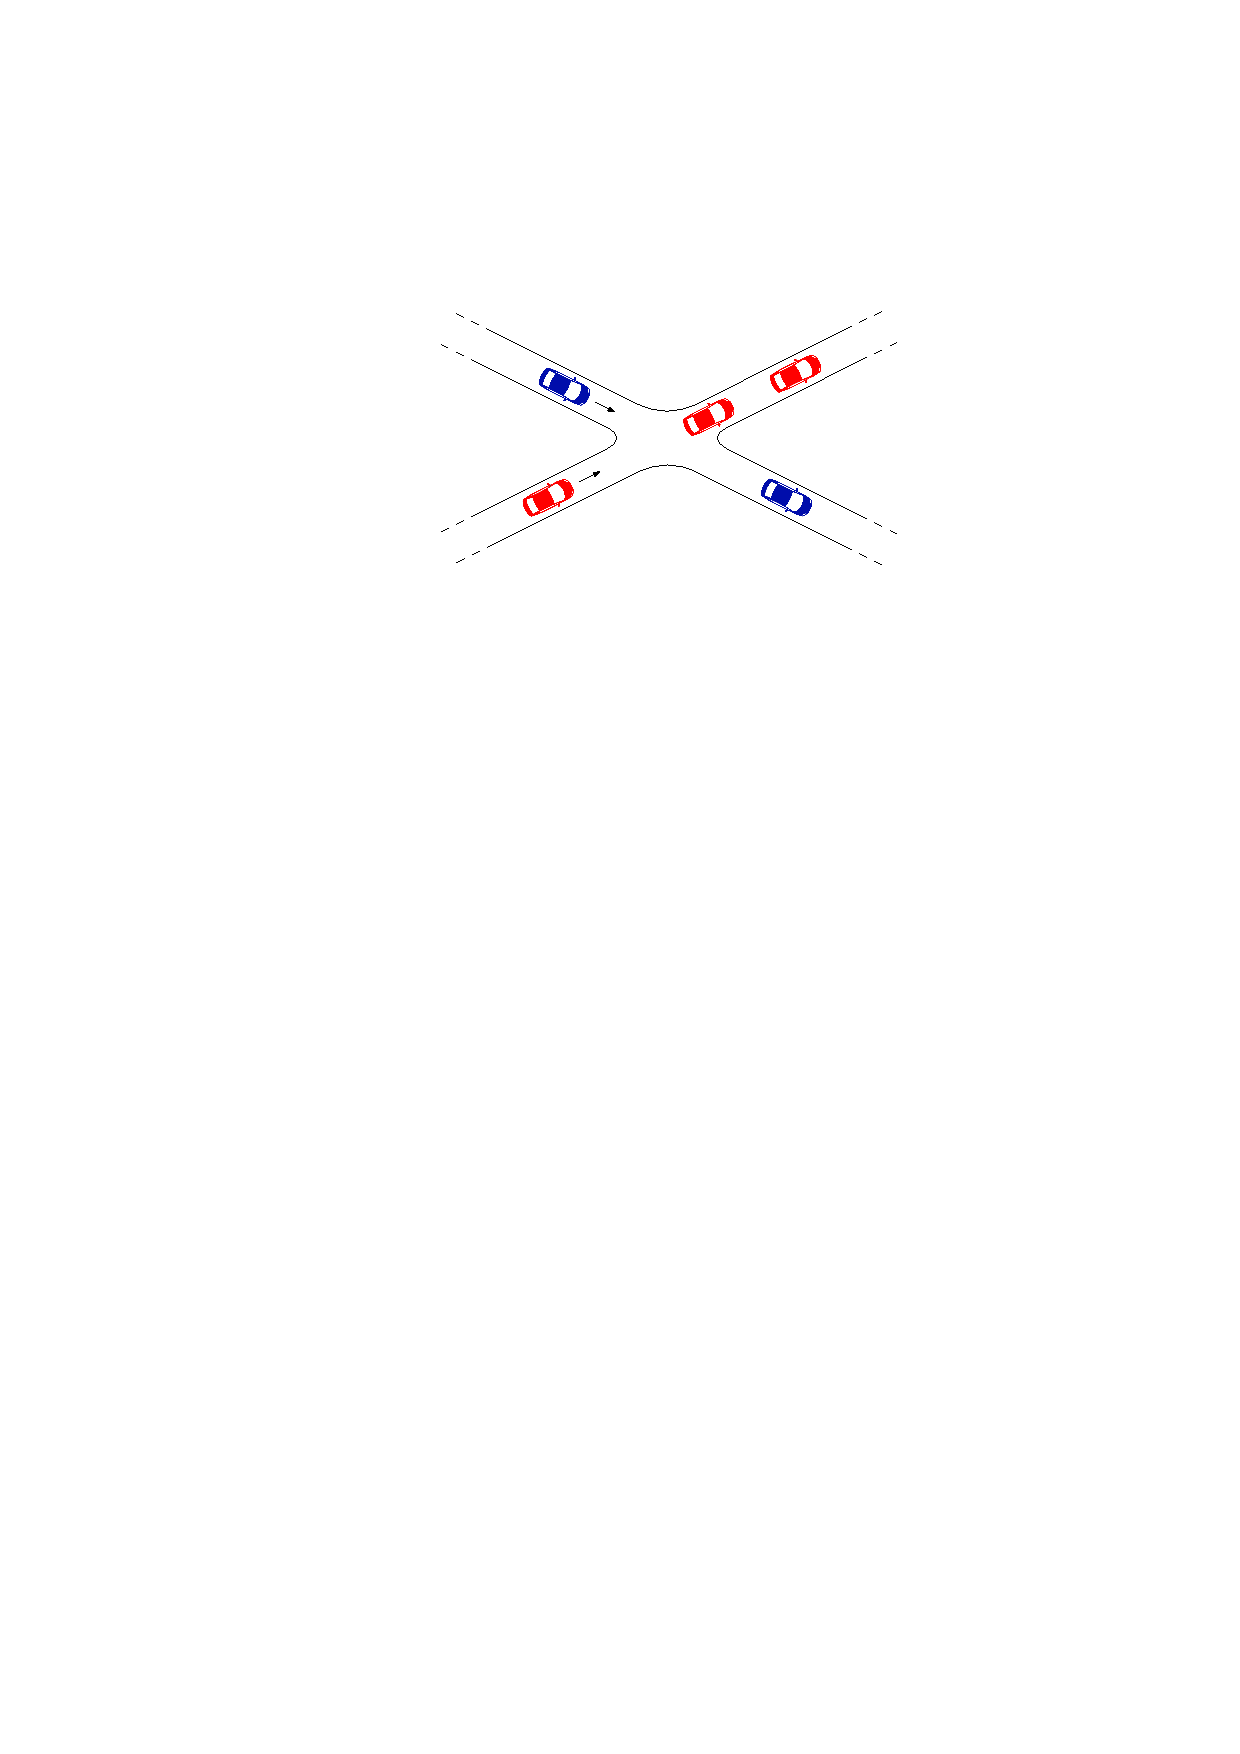
\includegraphics[scale=1]{figures/intersection-nice}
  \caption{Stylized model of a single intersection with two conflicting flows
    that do not merge, so we assume vehicles must cross the intersection in a
    straight line, without turning.}
\end{figure}


\paragraph{Crossing time scheduling.} We need to take a discrete decision regarding the
crossing order of vehicles at intersections. This remains true for any
generalization of the model to multiple lanes and intersections.
%
However, after fixing these ordering decisions, the remaining problem is often
much easier to solve. This observation motivates the decomposition of the
trajectory optimization problem into two parts.
%
The upper-level problem determines the times at which vehicles cross the
intersections on their routes, to which we will refer as \emph{crossing times}.
%
Once these are fixed, we solve a set of lower-level problems to find the
corresponding vehicle trajectories satisfying the crossing times.

Without additional assumptions, the upper-level problem is still as difficult as
before, because the feasibility of a crossing time schedule may depend on the
feasibility of the lower-level trajectory optimization problems in a non-trivial
way.
%
We will provide assumptions under which this coupling becomes particularly
simple.
%
Specifically, we show that feasibility of the lower-level problems can be states
as a system of linear inequalities in terms of the crossing times and we will
see that they also have simple interpretations.
%
This allows us to formulate the upper-level problem as a mixed-integer linear
problem that looks very similar to the classical job shop scheduling problem.

\paragraph{Learning to schedule.}

Because the lower-level problems can in general be solved efficiently, the
original trajectory optimization problem is essentially reduced to a scheduling
problem.
%
This enables us to explore some applictions of recent machine learning
techniques for such problems.
%
Specifically, the solution of a scheduling problem can be interpreted as a
sequence of decisions.
%
Instead of manually trying to develop good heuristics and algorithms, we try to
learn what optimal solutions are, by treating it as a learning task on
sequences.


\subsection{Related work}

We briefly survey some releated work that addressed coordination of autonomous
vehicles in a similar setting.
%
A good example of an early centralized approach
is the ``Autonomous Intersection Management'' (AIM)
paper~\cite{dresnerMultiagentApproachAutonomous2008}, which is based on a
reservation scheme. The conflict zone is modeled as a grid of cells. Vehicles
that want to cross the intersection send a request to the central controller to
occupy the cells containing its trajectory for a certain amount of time. The
central controller then decides to grant or deny these requests based on
previous granted requests, in order to facilitate collision-free trajectories.
If a request is denied, the vehicle slows down and attempts to obtain a new
reservation after some timeout.

% direct transcription
\paragraph{Direct transcription.}
Optimal control problems can be approached in an end-to-end fashion by
\textit{direct transcription} to an equivalent mixed-integer optimization
problem, which can be solved using off-the-shelf solvers (e.g.,
SCIP~\cite{BolusaniEtal2024OO} or Gurobi~\cite{gurobi}). Such methods can be
used to compute optimal trajectories up to any precision, by choosing a fine
enough time discretization. However, it is exactly this time discretization that
causes prohibitive growth of the number of variables with respect to the size of
the network and the number of vehicles, so this method is only useful for
relatively small problem instances.
%
Therefore, approximation schemes have been studied in previous
works~\cite{hultApproximateSolutionOptimal2015,zhaoBilevelProgrammingModel2021,tallapragadaHierarchicaldistributedOptimizedCoordination2017},
which we will review next.

\paragraph{Decomposition methods.}
% Hult et al. (offline single intersection with energy objective)
% "An approximate solution to the optimal coordination problem for autonomous
% vehicles at intersections"
The approximation method in~\cite{hultApproximateSolutionOptimal2015} is based
on a bilevel decomposition and considers a quadratic objective involving
velocity as a proxy for energy. The first stage optimizes a schedule of vehicle
crossing times. It uses approximations of each vehicle's contribution to the
total objective as a function of its crossing time. Next, for each vehicle, the
second stage computes an optimal trajectory satisfying the crossing time
schedule, by solving a quadratic program. This approach has been shown to reduce
running times significantly. Unfortunately, the study is limited to a single
intersection and it is assumed that each lane approaching the intersection
contains exactly one vehicle.
% Zhao et al. (bilevel programming model)
The paper~\cite{zhaoBilevelProgrammingModel2021} proposes a trajectory
optimization scheme for a single intersection, also based on the bilevel
decomposition. The lower-level problem is employed to maximize the speed at
which vehicles enter the intersection. Both parts of the problem are solved in an alternating
fashion, each time updating the constraints of the other part based on the
current solution.
% bubbles paper
The optimization scheme
in~\cite{tallapragadaHierarchicaldistributedOptimizedCoordination2017} deals
explicitly with the complexity of the crossing order decisions by defining
groups of consecutive vehicles on the same lane. The first step is to group
vehicles into these so-called ``bubbles''. All vehicles in a bubble are required
to cross the intersection together, while maintaining feasibility with respect
to safe trajectories. Next, crossing times are assigned to bubbles while
avoiding collisions. Based on this schedule, a local vehicular control
method~\cite{tallapragadaDistributedControlVehicle2017} is used that guarantees
safety to reach the assigned crossing times.


\subsection{Contributions and outline}

This thesis is centered around the following two main contributions:

\paragraph{(i). Decomposition.}
Our first contribution is to show that, under certain conditions, our joint
trajectory optimization problem for vehicles in a network of intersections
decomposes into an upper-level crossing time scheduling problem and a set of
lower-level trajectory optimization problems. We show that feasibility of the
upper-level scheduling problem is completely characterized in terms of a system
of linear inequalities involving the crossing times. This allows us to first
solve the scheduling problem and then generate trajectories for it once we have
the optimal crossing time schedule.

\paragraph{(ii). Learning to schedule.}
Our second contribution is an illustration of how machine learning techniques
can be applied to solve scheduling problems in practice.
%
Many practical instances contain structure that classic solutions techniques try
to exploit, e.g., by defining smart heuristics based on human intuition and
experience.
%
We aim to automated this manual endeavor by formulating parameteric sequence
models to capture the conditional probability of optimal solutions, given a
problem instance.
%
As has been noted before, we confirm that the order of evaluation during
inference matters a lot for the final solution quality.

\paragraph{Outline.}

The rest of this chapter discusses some preliminaries: we briefly discuss the
job shop scheduling problem in, because our crossing time scheduling problem may
be seen as an extension; we provide a brief overview of how machine learning
methods can be applied to solve combinatorial optimization problems, with a
focus on job shop scheduling.
%
In Chapter~\ref{chap:single}, we consider a simple model of a single
intersection, like the example above. After discussing the decomposition method,
we present some classical solutions methods to solve the crossing time
scheduling problem.
%
We explain how the problem can be treated as a learning problem in
Chapter~\ref{chap:single-learning}.
%
In order to generalize to a network of intersections, we need to precisely study
the feasibility of trajectories in lanes of finite length, which is done in
Chapter~\ref{chap:network}.
%
The resulting scheduling problem is then subjected to a learning algorithm in
Chapter~\ref{chap:network-learning}.
%
We provide some general discussion and pointers for further research in
Chapter~\ref{chap:conclusion}.

\newpage
\section{Literature review}

\newcolumntype{L}[1]{>{\RaggedRight\hsize=#1\hsize\hspace{0pt}}X}
\begin{table}[t]
\centering
\renewcommand{\arraystretch}{1.2}

\begin{adjustbox}{center}
\scalebox{0.7}{
\begin{tabularx}{2.0\textwidth}{@{} l L{0.6} L{0.55} L{0.55} L{0.55} L{0.55} L{0.55} L{1.0} @{}}
\toprule
\textbf{Ref.} &
\textbf{Paradigm} &
\textbf{Dynamics} &
\textbf{Safety} &
\textbf{Objective} &
\textbf{Decision set} &
\textbf{Communication} &
\textbf{Notes / Limitations} \\
\midrule
\cite{dresnerMultiagentApproachAutonomous2008} &
Reservation-based &
Planar vehicle kinematics &
Conflict exclusion (grid cells) &
Delay minimization &
Entry times/reservation slots &
Multiagent with central intersection manager &
Simplified vehicle model; global heuristic \\
\bottomrule
\end{tabularx}}
\end{adjustbox}
\caption{Comparison of approaches to signal-free intersection management.}
\label{tab:litreview}
\end{table}


\newpage
\section{Job shop scheduling}\label{sec:job-shop}

The job shop model provides a mathematical framework to study systems where a
given set of---possibly distinct---facilities must be shared among a number of
heterogenous tasks over time.
%
We begin by providing a fairly general definition of this model and then present a
small example for a specific problem.
%
Next, we introduce the disjunctive graph, which is a standard auxiliary
representation of both problem instances and solutions.
%
Finally, we briefly discuss simple heuristics and illustrate how job shop
problems can be approached within the mixed-integer programming framework.
%
For a comprehensive textbook treatment of job shop scheduling, we refer the
reader to~\cite[Chapter 7]{pinedoSchedulingTheoryAlgorithms2016}.

\paragraph{General definition.}
Originally motivated by production planning problems, the job shop model is
phrased in terms of a set of $n$ jobs that require to be processed on a set of
$m$ machines. Each machine can process at most one job at the same time.
%
We use the pair of indices $(i,j)$ to identify the operation that machine $i$
performs on job $j$, which takes a fixed amount of time $p(i,j)$.
%
Each job $j$ visits all machines\footnote{When some job $j$ requires only
  processing on a proper subset of the machines, observe that we can simply
  assume that $p(i,j) = 0$ for each machine $i$ that is not involved.} following
a predetermined machine sequence, which may be different among jobs.
%
Let $\mathcal{N}$ denote the set of all operations, then the general Job Shop Scheduling
Problem (JSSP) is to determine a schedule $y = \{ y(i,j) : (i,j) \in \mathcal{N} \}$ of
starting times such that some objective function $J(y)$ is minimized.
%
Variants of this basic problem can be obtained by specifying a concrete
objective function and by introducing additional constraints, which we will both
illustrate in the following example.

\begin{eg}\label{eg:job-shop}
  Let $s_{j}$ and $e_{j}$ denote the first and last machine that job $j$ vists, respectively.
  %
  For each job $j$, we define a so-called release date $r(j)$ by requiring that
  $y(s_{j},j) \geq r(j)$.
  %
  As objective function, we consider the so-called makespan
  $J(y) := \max_{j} y(e_{j},j) + p(e_{j}, j)$, which we aim to minimize.
  %
  The resulting problem is known as $Jm|r_{j}|C_{\max}$ in the commonly used
  three-field classification notation~\cite{grahamOptimizationApproximationDeterministic1979}, see also~\cite[Chapter
  2]{pinedoSchedulingTheoryAlgorithms2016}.
  %
  Now consider a specific problem instance with $m=3$ machines and $n=2$ jobs.
  We specify the order in which jobs visit machines by providing the
  corresponding ordering of operations, which we choose to be
  $(1,1) \rightarrow (2,1) \rightarrow (3,1)$ and $(3,2) \rightarrow (2,2) \rightarrow (1,2)$. Using matrix notation
  $r(j) \equiv r_{j}$ and $p(i,j) \equiv p_{ij}$, the release dates and processing
  times are given by
  \begin{align*}
    r =
    \begin{pmatrix}
      1 & 0
    \end{pmatrix} ,
    \quad\quad
    p =
    \begin{pmatrix}
      2 & 1 \\
      1 & 3 \\
      4 & 1
    \end{pmatrix} .
  \end{align*}
  For this problem, Figure~\ref{fig:job-shop-delay} shows an optimal schedule $y^{*}$ with
  makespan $J(y^{*}) = 8$.
\end{eg}

\begin{figure}
  \centering
  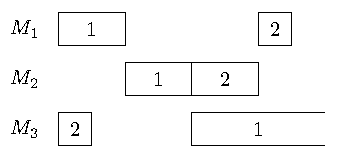
\includegraphics[scale=1]{figures/job-shop-delay.pdf}
  \caption{Example of an optimal schedule for Example~\ref{eg:job-shop}, shown
    as a Gantt chart. Each row $M_{i}$ corresponds to machine $i$ and each block
    numbered $j$ on this row represents the operation $(i,j)$. The dashed lines
    indicate unit time steps. Note that machine 2 is kept idle, while operation
    $(2,2)$ could have already been scheduled at time 1. Furthermore, for this
    particular instance, it can be checked that this is the unique optimal
    schedule.}
  \label{fig:job-shop-delay}
\end{figure}

\paragraph{Disjunctive graph.}

A commonly used representation of job shop problems is through their disjunctive
graph, which is a directed graph with vertices $\mathcal{N}$ corresponding to the
operations and two types of arcs.
%
The conjunctive arcs $\mathcal{C}$ are used to encode the predetermined machine
sequence of each job. Each such arc $(i, j) \rightarrow (k, j)$ encodes that job
$j$ should first be processed on machine $i$ before it is processed on machine
$k$.
%
When two distinct jobs $j_{1}$ and $j_{2}$ both require processing on the same
machine $i$, we say that they are conflicting.
%
The disjunctive arcs $\mathcal{D}$ are used to encode the possible choices of
resolving such conflicts, by deciding which of $j_{1}$ or $j_{2}$ visits $i$
first.
%
More specifically, let $j_{1}$ and $j_{2}$ be conflicting on some machine $i$,
then the nodes $(i,j_{1})$ and $(i,j_{2})$ are connected by two arcs in opposite
directions.

The disjunctive graph can also be used to encode (partial) solutions as follows.
%
It can be shown that each feasible solution corresponds to a selection
$\mathcal{O}$ of exactly one disjunctive arc from each pair such that the
induced graph $(\mathcal{N}, \mathcal{C} \cup \mathcal{O})$ is
acyclic~\cite{pinedoSchedulingTheoryAlgorithms2016}.
%
More precisely, consider two conflicting operations $(i,j_{1})$ and $(i,j_{2})$,
then $\mathcal{O}$ contains either $(i,j_{1}) \rightarrow (i,j_{2})$ or
$(i,j_{1}) \rightarrow (i,j_{2})$.
%
To illustrate this, the empty and complete disjunctive graphs for the instance
in Example~\ref{eg:job-shop} are shown in Figure~\ref{fig:disjunctive-graphs}.

\begin{figure}
  \centering
  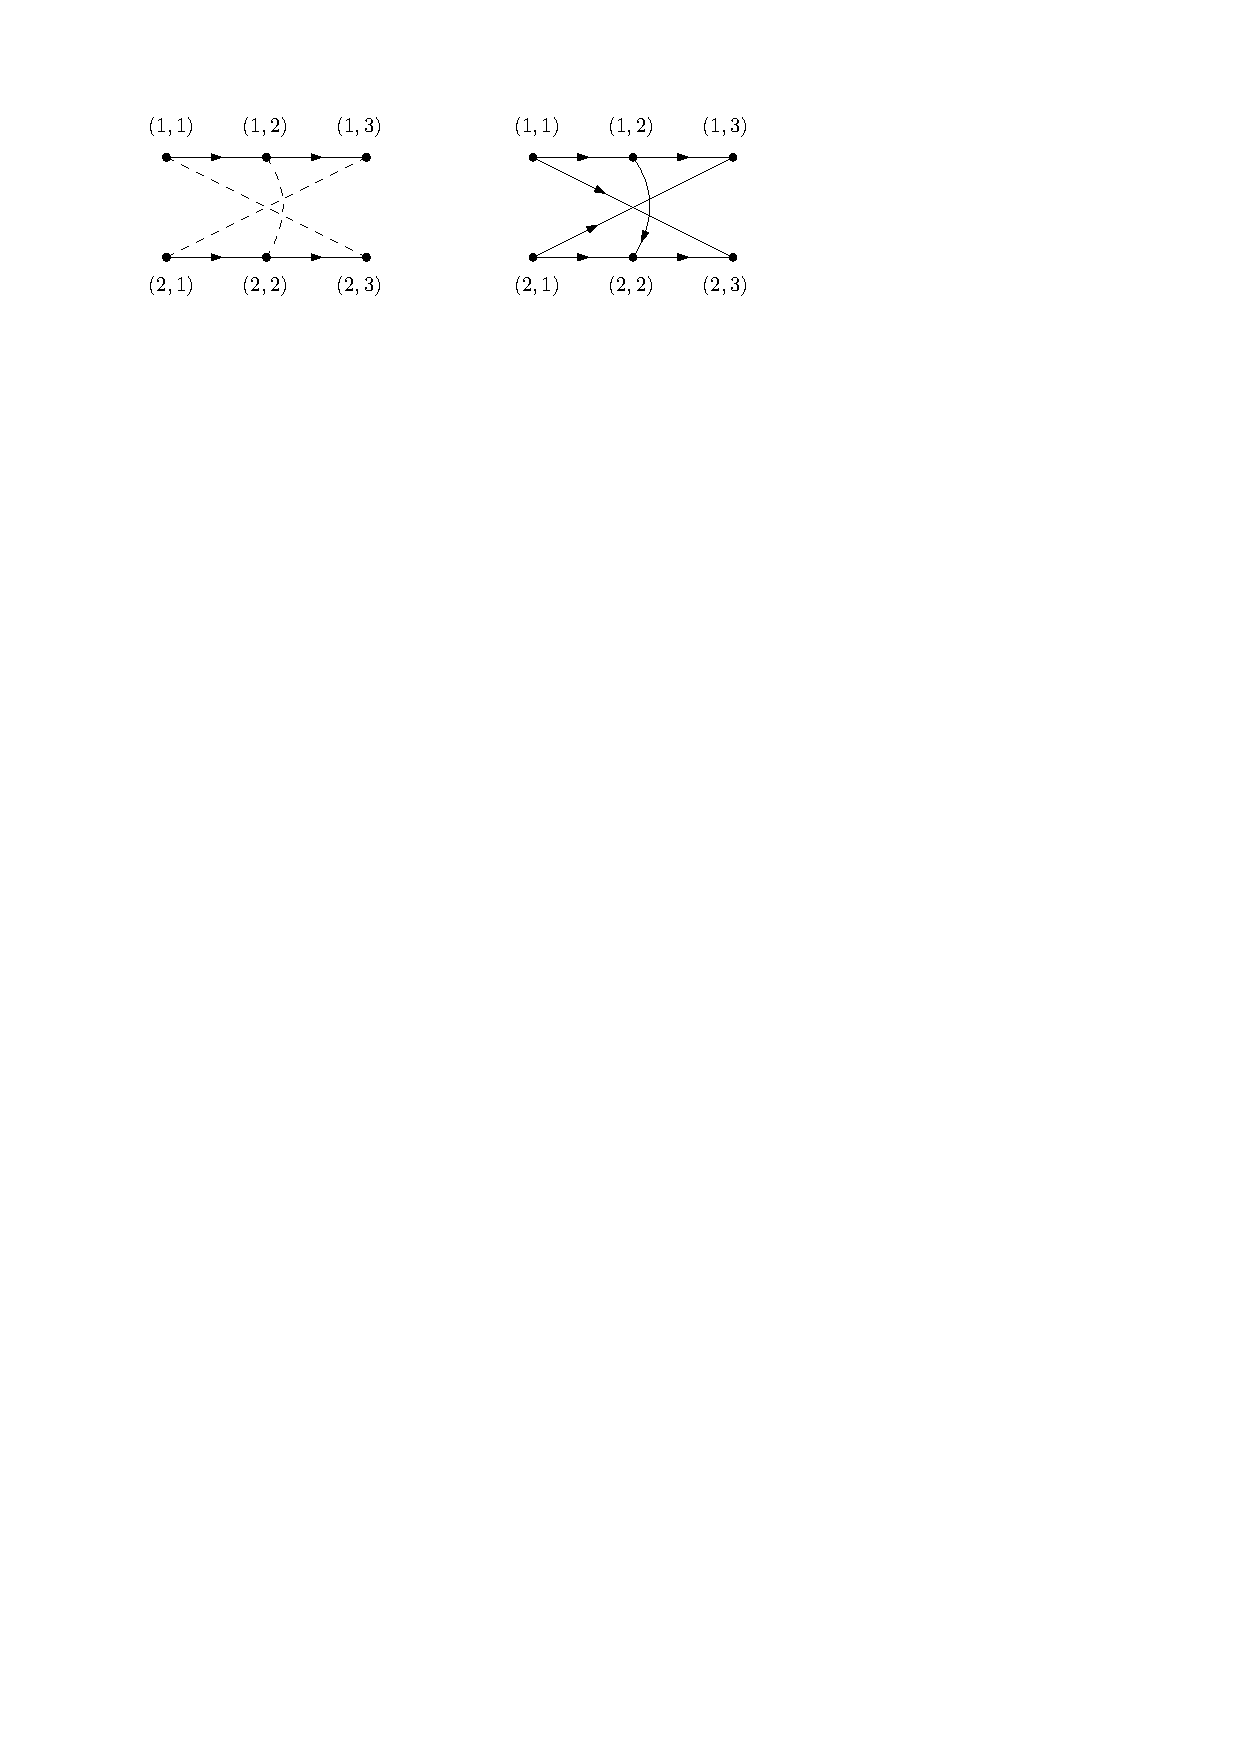
\includegraphics[scale=1]{figures/disjunctive_graph.pdf}
  \caption{Illustration of disjunctive graphs for Example~\ref{eg:job-shop}.
    Horizontal arrows represent conjunctive arcs. We used dashed lines to for
    the pairs of disjunctive arcs as dashed lines. The left graph corresponds to
    an empty selection $\mathcal{O} = \varnothing$ while the right graph shows
    the selection $\mathcal{O}$ that corresponds to the optimal schedule of
    Figure~\ref{fig:job-shop-delay}.}
  \label{fig:disjunctive-graphs}
\end{figure}


\paragraph{Solution methods.}

Most job shop problems are very hard to solve. For example, the class of
problems $Jm|r_{j}|C_{\max}$ considered in Example~\ref{eg:job-shop} is known to
be NP-hard~\cite{grahamOptimizationApproximationDeterministic1979}, even without
release dates, which is denoted $Jm||C_{\max}$.
%
As a consequence, much effort has gone into developing good heurstics.
%
A type of heuristic that is often considered is to apply a so-called \emph{dispatching
rule} in order to build a schedule in a step-by-step fashion.
%
At each step, the rule chooses some job from all jobs with remaining unscheduled
operations and schedules this next operation at the earliest time possible,
given the current schedule.

A more principled way of solving job shop problems relies on the mathematical
programming framework.
%
We illustrate this for the problem $Jm|r_{j}|C_{\max}$ of
Example~\ref{eg:job-shop}. Using the notation of the disjunctive graph, the
problem can be concisely stated as
\[
\renewcommand{\arraystretch}{1.2}
\begin{NiceArray}{ r l @{} >{{}}c<{{}} @{} l @{} }
  \displaystyle \min_{y} & J(y) \\
  \text{such that } \; & y(s_{j},j) \leq r(j) && \quad \text{ for each job } j , \\
  &y(i, j) + p(i, j) \leq y(r, k) && \quad \text{ for each conjunction } (i,j) \rightarrow (r,k) \in \mathcal{C} , \\
  & y(i,j) + p(i,j) \leq y(i,k) & \\
  & \hspace{2em} \text{ or (not both) } && \quad \text{ for each disjunction } (i,j) \leftrightarrow (i,k) \in \mathcal{D} , \\
  & y(i,k) + p(i,k) \leq y(i,j) \\
  & y(i,j) \in \mathbb{R} && \quad \text{ for each operation } (i,j) .
\CodeAfter\SubMatrix.{4-1}{6-2}\}
\end{NiceArray}
\]
%
Note that this is almost an mixed-integer linear program (MILP).
%
Let $M > 0$ be some sufficiently large number and introduce a binary decision
variable $b_{(i,j)\leftrightarrow (i,k)} \in \{0,1\}$ for each pair of
disjunctive arcs, then the pair of disjunctive constraint can be rewritten to
\begin{align*}
  y(i,j) + p(i,j) &\leq y(i,k) + M b_{(i,j)\leftrightarrow (i,k)} , \\
  y(i,k) + p(i,k) &\leq y(i,j) + M (1 - b_{(i,j)\leftrightarrow (i,k)}) ,
\end{align*}
which is generally refered to as the \emph{big-M method}. The resulting MILP can
be solved by any off-the-shelf solver, e.g., we used the commerical Gurobi
Optimizer software~\cite{gurobi} for this thesis.

\section{Reinforcement learning}

For machine learning problems where data-collection is restricted in some way,
the supervised learning paradigm, i.e., learning from labeled examples, is
sometimes no longer appropriate or feasible.
%
Very generally, the reinforcement learning paradigm can viewed as a
generalization of supervised learning in which the data collection and selection
process is not fixed anymore.
%
The classical perspective is that of an \emph{agent} that tries to maximize some
cumulative \emph{rewward} signal when interacting in some \emph{environment},
which is formalized by the Markov Decision Process (MDP) model.
%
We refer the reader to~\cite{suttonReinforcementLearningIntroduction2018} for the commonly cited textbook introduction to RL
from this perspective.

\paragraph{Problem definition.}
Consider finite sets of states $\mathcal{S}$ and actions $\mathcal{A}$.
%
Given some current state $s$, the agent sends some action $a$ to the
environment, upon which it responds by providing some scalar reward signal $r$
and transitions to state $s'$, which happens with probablity $p(s', r | s, a)$.
%
By fixing a policy $\pi$, which is a function $\pi(a|s)$ that gives the
probablity of the agent choosing action $a$ in state $s$, we obtain the induced
\emph{state Markov chain} with transition probabilities
%
\begin{align*}
  \mathrm{Pr}(s \rightarrow s') = \sum_{a} \sum_{r} \pi(a|s) p(s', r | s, a) .
\end{align*}
Given some initial state distribution $h(s)$, we sample $S_{0} \sim h(s)$ and
use $S_{0}, S_{1}, S_{2}, \dots$ to denote some sample trajectory.
%
Moreover, we can also consider a more fine-grained Markov chain by considering
the sequence of states, actions and rewards
\begin{align*}
  S_{0}, A_{1}, R_{1}, S_{1}, A_{2}, R_{2}, S_{2}, \dots ,
\end{align*}
in which which the state Markov chain is naturally embedded. Such a sample
trajectory is also refered to as an \emph{episode}.
%
Let the corresponding \emph{return} at step $t$ be
defined as
\begin{align*}
  G_{t} = \sum_{k=t+1}^{\infty} R_{k} .
\end{align*}
By marking a subset of states as being \emph{final states}, we can consider finite episodes
\begin{align*}
  S_{0}, A_{1}, R_{1}, S_{1}, A_{2}, R_{2}, S_{2}, \dots S_{N},
\end{align*}
by using the convention that final states return zero reward and transition to
themselves almost surely.
%
For finite episodes, the goal is to find a policy $\pi$ that maximizes the
expected return $\mathbb{E}[G_{0}]$.

\paragraph{Solution methods.}
Most classical methods to find such an optimal policy $\pi$ can be categorized
as either being value-based or policy-based.
%
Value-based can be generally understood as producing some estimate $v(s)$ for
the expected return $\mathbb{E}[G_{0} | S_{0} = s]$. The optimal policy is then
parameterized in terms of these estimates $v(s)$.
%
In contrast, policy-based methods use a more direct parameterization of the
policy space and often rely on some kind of gradient-based optimization.
Specifically, let $\pi_{\theta}$ be some policy with parameters $\theta$, then we aim to
apply the gradient descent updating
\begin{align*}
  \theta \leftarrow \theta - \alpha \nabla \mathbb{E} [ G_{0} ]
\end{align*}
where $\alpha$ is refered to as the learning rate.
%
However, in almost all interesting situations, it is infeasible to compute the
gradient directly.

\section{Neural combinatorial optimization}

% maybe discuss traditional epsilon-approximation schemes?
% argue that it takes a lot of expert knowledge about the problem structure to design these

This section introduces the idea of applying a Machine Learning (ML) perspective
on Combinatorial Optimization (CO) problems, which has gained a lot of
attention recently. One of the key ideas in this line of research is to treat problem
instances as data points and to use machine learning methods to approximately
map them to corresponding optimal solutions~\cite{bengioMachineLearningCombinatorial2020}.

% learning assumptions:
% supervised learning (expert labels) vs reinforcement learning (experience)
\paragraph{Algorithm execution as MDPs.}
It is very natural to see the sequential decision-making process of any
optimization algorithm in terms of the MDP framework, where the environment
corresponds to the internal state of the algorithm. From this perspective, two
main learning regimes can be distinguished.
% imitiation learning
Methods like those based on the branch-and-bound framework are
often computationally too expensive for practical purposes, so \textit{learning
  to imitate} the decisions taken in these exact algorithms might provide us
with fast approximations. In this approach, the ML model's performance is
measured in terms of how similar the produced decisions are to the
demonstrations provided by the expert.
% reinforcement learning
On the other hand, some problems do not even allow efficient exact methods, so it is
interesting to study solution methods that \textit{learn from experience}. An
interesting feature of this direction is that it enables the algorithm to implicitly
learn to exploit the hidden structure of the problems we want to solve.

% neural combinatorial optimization
Because neural networks are commonly used as encoder in these ML models for CO,
we will refer to this new field as \textit{Neural Combinatorial Optimization} (NCO).
%
A wide range of classical combinatorial optimization problems has already been
considered in this framework, so we briefly discuss the taxonomy used in the
survey~\cite{mazyavkinaReinforcementLearningCombinatorial2020}.
% principal vs. joint approach
One distinguishing feature is whether existing off-the-shelf solvers are used or
not. On the one hand, \textit{principal} methods are based on a parameterized algorithm
that is tuned to directly map instances to solutions, while \textit{joint} methods
integrate with existing off-the-shelf solvers in some way (see the
survey~\cite{lodiLearningBranchingSurvey2017} on integration with the
branch-and-bound framework). An illustrative example of the latter category are
the use of ML models for the branching heuristic or the selection of cutting
planes in branch-and-cut algorithms~\cite{tangReinforcementLearningInteger2020}.
% principal - construction vs. improvement (guided search)
The class of principal methods can be further divided into \textit{construction}
heuristics, which produce complete solutions by repeatedly extending partial
solutions, and \textit{improvement} heuristics, which aim at iteratively improving the
current solution with some tunable search procedure.


% learning algorithms:
% REINFOCE with baseline
% Fitting the neural mapping is often done using policy gradient methods (with
% baseline), e.g., with the classical REINFORCE algorithm.

% constraints in differentiable models

\paragraph{Constraint satisfaction.}
A major challenge in NCO is constraint
satisfaction. For example, solutions produced by neural construction policies
need to satisfy the constraints of the original combinatorial problem.
To this
end, neural network components have been designed whose outputs satisfy some
specific type of constraint, for example being a permutation of the
input~\cite{vinyalsPointerNetworks2017a}. Constraints can also be enforced by
the factorization of the mapping into repeated application of some policy. For
example, in methods for TSP, a policy is defined that repeatedly selects the
next node to visit. The constraint that nodes may only be visited once can be
easily enforced by ignoring the visited nodes and taking the argmax among the
model's probabilities for unvisited nodes.

% encoders:
% standard multilayer perceptron networks are not suited to encode order
% pointer networks
% graph neural networks

% backpropagation through solution
Instead of enforcing constraints by developing some tailored model architecture,
like construction and improvement heuristics, general methodologies have
recently been explored for the problem of constraint satisfaction in neural
networks. For example, the DC3 framework~\cite{dontiDC3LearningMethod2021}
employs two differentiable processes, completion and correction, to solve any
violations of equality or inequality constraints, respectively. The more recent
HardNet framework~\cite{minHardConstrainedNeuralNetworks2024} uses a closed-form
projection to map to feasible solutions under affine constraints and relies on a
differentiable convex optimization solver (e.g.,
OptNet~\cite{amosOptNetDifferentiableOptimization2021a}) when general convex
constraints are considered.

\subsection{Neural job shop scheduling}

% examples for job-shop scheduling
Various NCO methods have already been studied for JSSP with makespan objective,
of which we now highlight some works that illustrate some of the above classes
of methods. A lot of the policies used in these works rely on some graph neural
network architecture, which is why the survey~\cite{smitGraphNeuralNetworks2024}
provides an overview based on this distinguishing feature.

% Tassel (principal construction, naive environment)
\paragraph{Dispatching rules.}
A very natural approach to model JSSP in terms of an MDP is taken
in~\cite{tasselReinforcementLearningEnvironment2021}, where a dispatching
heuristic is defined in an environment based on discrete scheduling time steps.
%
Every available job corresponds to a valid action and there is a so-called No-Op
action to skip to the next time step. States are encoded by some manually
designed features. They consider the makespan objective by proposing a dense
reward based on how much idle time is introduced compared to the processing time
of the job that is dispatched.
%
In some situation, some action can be proved to be always optimal (``non-final
prioritization''), in which case the policy is forced to take this action.
Additionally, the authors design some rules for when the No-Op action is not
allowed in order to prevent unnecessary idling of machines.
%
The proposed method is evaluated on the widely used
Taillard~\cite{taillardBenchmarksBasicScheduling1993} and
Demirkol~\cite{DEMIRKOL1998137} benchmarks, for which performance is compared to
static dispatching rules and a constraint programming (CP) solver, which is
considered cutting-edge.

% exact start times follow from order
From a scheduling theory
perspective~\cite{pinedoSchedulingTheoryAlgorithms2016}, it can be shown that
optimal schedules are completely characterized by the order of operations for
regular objectives (non-decreasing functions of the completion times). The start
times are computed from this order by a so-called \textit{placement rule}, so
considering discrete time steps introduces unnecessary model redundancy.

% Zhang construction heuristic (principal construction, based on order)

The seminal ``Learning to Dispatch'' (L2D)
paper~\cite{zhangLearningDispatchJob2020} proposes a construction heuristic for
JSSP with makespan objective. Their method is based on a dispatching policy that
is parameterized in terms of a graph neural network encoding of the disjunctive
graph belonging to a partial solution. Again, each action corresponds to
choosing for which job the next operation is dispatched. The rewards are based
on how much the lower bound on the makespan changes between consecutive states.
They use a Graph Isomorphism Network (GIN) architecture to parameterize both an
actor and critic, which are trained using the Proximal Policy Optimization (PPO)
algorithm. Using the Taillard and Demirkol benchmarks, they show that their
model is able to generalize well to larger instances.
% problem with dispatching mechanism
As we already alluded to above, this way of modeling the environment is better
suited to JSSP with regular objectives, because it does not explicitly determine
starting times.
%
They use a dispatching mechanism based on finding the earliest starting time of
a job, even before already scheduled jobs, see their Figure 2. By doing this,
they introduce symmetry in the environment: after operations
$O_{11}, O_{21}, O_{31}$ have been scheduled, both action sequences
$O_{22}, O_{32}$ and $O_{32}, O_{22}$ lead to exactly the same state $S_5$ shown
in their Figure 2. In this particular example, this means that it is impossible
to have $O_{11} \rightarrow O_{22} \rightarrow O_{32}$. In general, it is not
clear whether the resulting restricted policy is still sufficiently powerful, in
the sense that an optimal operation order can always be constructed.

% Zhang improvement heuristic (principal improvement)

\paragraph{Guided local search.}
Recently, the authors of L2D investigated an improvement heuristic for
JSSP~\cite{zhangDeepReinforcementLearning2024} with makespan objective.
%
This method is based on selecting a solution within the well-known $N_5$
neighborhood, which has been used in previous local search heuristics.
%
It is still not clear whether their resulting policy is complete, in the sense
that any operation order can be achieved by a sequence of neighborhood moves.
%
The reward is defined in terms of how much the solution improves relative to the
best solution seen so far (the ``incumbent'' solution). The policy is
parameterized using a GIN architecture designed to capture the topological
ordering of operations encoded in the disjunctive graph of solutions. They
propose a custom $n$-step variant of the REINFORCE algorithm in order to deal
with the sparse reward signal and long trajectories.
%
To compute the starting times based on the operation order, they propose a
dynamic programming algorithm, in terms of a message-passing scheme, as a more
efficient alternative to the classical recursive critical path method.
%
Our proposal for efficiently updating the current starting time lower bounds in
partial solutions can also be understood as a similar message-passing scheme,
but where only some messages are necessary.

\paragraph{Joint method.}
% Tassel (joint with CP solver)
An example of a joint method is given
in~\cite{tasselEndEndReinforcementLearning2023}, where the environment is stated
in terms of a Constraint Programming (CP) formulation. This allows the method to
be trained using demonstration from an off-the-shelf CP solver.


\microtypesetup{deactivate}
\part*{\hspace*{-0.8em}\textsc{Part I}\\[0.6em] Single Isolated Intersection\\[3em]
       \centering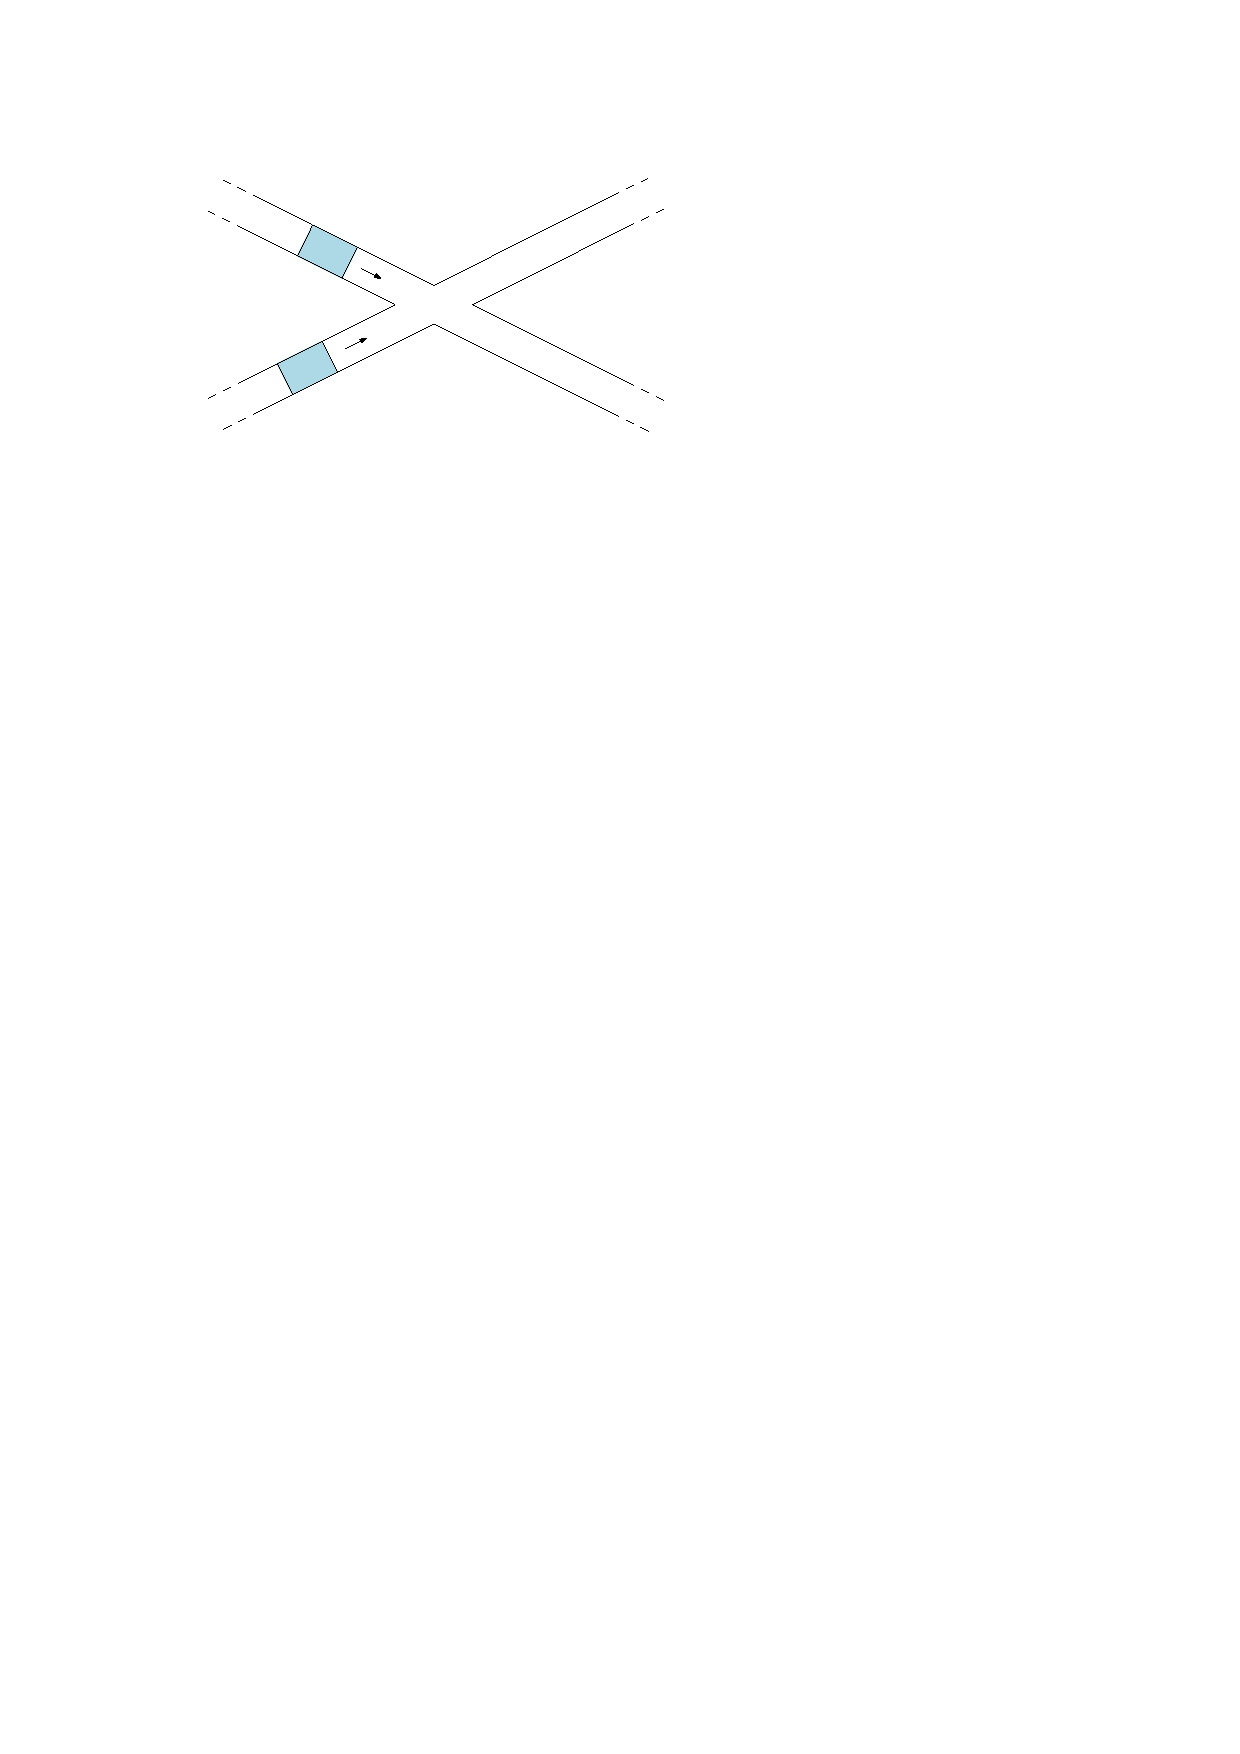
\includegraphics[scale=1]{figures/intersection-non-axis-aligned}}
\microtypesetup{activate}
\addcontentsline{toc}{part}{Part I \;--\; Isolated Intersection}



\chapter{Isolated intersection scheduling}\label{chap:single}

% broad problem:
% - why intersections matter in traffic coordination
% - why coordination is interesting

% simpflified model as a tractable starting point
% assumptions:
% - two lanes
% - perpendicular
% - no turning
% - no overtaking
% - homogeneous vehicles (same dimensions and dynamics)
% - no randomness
%  - fixed

% optimization objective:
%   - energy consumption -> very desirable on top of delay, but makes analysis difficult
%   - travel delay -> essential, enables problem simplification (decomposition)

% mathematical punchline:
% - first, it becomes a trajectory optimization problem (optimal control)
%   - can be solved directly
% - next, we turn it into a very simple scheduling (when) / sequencing (only order) problem

% preview of results:
% - mention direct transcription
% - main takeaway: bilevel decomposition
% - branch-and-cut solution
%   - problem structure yields cutting planes
%   - analye performance improvement
% - optionally, mention local search

% broad problem
Efficient coordination of vehicle motion at intersections is one of the central
challenges in traffic management, since intersections are natural bottlenecks
where safety requirements and efficiency objectives are directly in conflict.
%
With the advent of automated vehicles and reliable wireless communication
technologies, there is increasing potential to replace traditional traffic
signal-based approaches with coordinated trajectory planning methods.
%
As a first step toward analyzing such methods, this chapter focuses on a
simplified single-intersection setting in which vehicles follow fixed routes and
are centrally controlled to optimize traffic flow while guaranteeing safety.

% model assumption to make analysis tractable
To make the analysis tractable, we restrict attention to an intersection formed
by two perpendicular lanes, with vehicles traveling straight through, without allowing
turning maneuvers or overtaking.
%
All vehicles are assumed to be homogeneous, sharing identical dimensions and
dynamics, so that their motion can be modeled uniformly.
%
A central controller determines the acceleration, and thus the speed, of each
vehicle, under the assumption of perfect communication.
%
Moreover, we do not consider randomness in arrivals or dynamics, so we assume
that each vehicle's initial state is known precisely such that the system
evolves deterministically as a function of the acceleration control inputs.

% optimization objectives
Within this setting, two performance objectives are of primary interest.
%
Minimizing energy consumption is highly desirable in practice, as it directly
contributes to the sustainability benefits of automated traffic systems.
%
However, incorporating energy makes analysis significantly more complex.
%
By contrast, minimizing travel delay is essential for capturing the efficiency
of traffic flow and, importantly, we will see that it enables a very useful
problem decomposition.
%
For these reasons, the focus of this chapter is primarily on minimizing delay,
while recognizing energy consumption as a complementary objective.

% mathematical punchline
Formulated mathematically, the coordination problem at the intersection can be
expressed as a problem of \emph{trajectory optimization}, or optimal control.
%
In this formulation, the accelerations of all vehicles are chosen to satisfy
their dynamic constraints and collision-avoidance requirements while minimizing
the chosen performance objective.
%
Such problems can in principle be solved directly using standard numerical
optimization techniques.
%
However, by exploiting the structure of the intersection model, we show that the
problem can be reduced to a much simpler form: a \emph{scheduling problem}, in which
only the sequencing of vehicles and their entry times into the intersection need
to be determined.


% preview of results
% \paragraph{Outline.}
The results presented in this chapter illustrate both perspectives.
%
After precisely formulating our model, we first apply a direct transcription
approach to the trajectory optimization problem, demonstrating how it can be
solved numerically in its original form.
%
The main contribution, however, is stating assumptions for which the trajectory
problem allows a bilevel decomposition in which the scheduling problem provides
\pagebreak
high-level sequencing and timing decisions, while a continuous trajectory
planning routine resolves the underlying vehicle dynamics.
%
To solve the scheduling component, we apply the branch-and-cut framework and
leverage the problem structure to generate effective cutting planes, leading to
significant performance improvements.
%
Finally, we mention the possible role of local search heuristics in refining
solutions.

\begin{remark}
  We will consider a continuous-time trajectory optimization problem, which is
  typically studied in the framework of optimal control theory. However, as the
  author does not have a strong background in this field, the aim is not to
  provide a rigorous treatment from this perspective. Nevertheless, at some
  points remarks are included regarding the difficulties of such analysis, most
  notably, regarding the occurence of so-called state constraints.
  %
  \note{Although the theory for dealing with state constraints (\`a la
    Pontryagin) is far from complete, in practice, they can be successfully
    dealt with in numerical approaches.}
\end{remark}

\begin{figure}
  \centering
  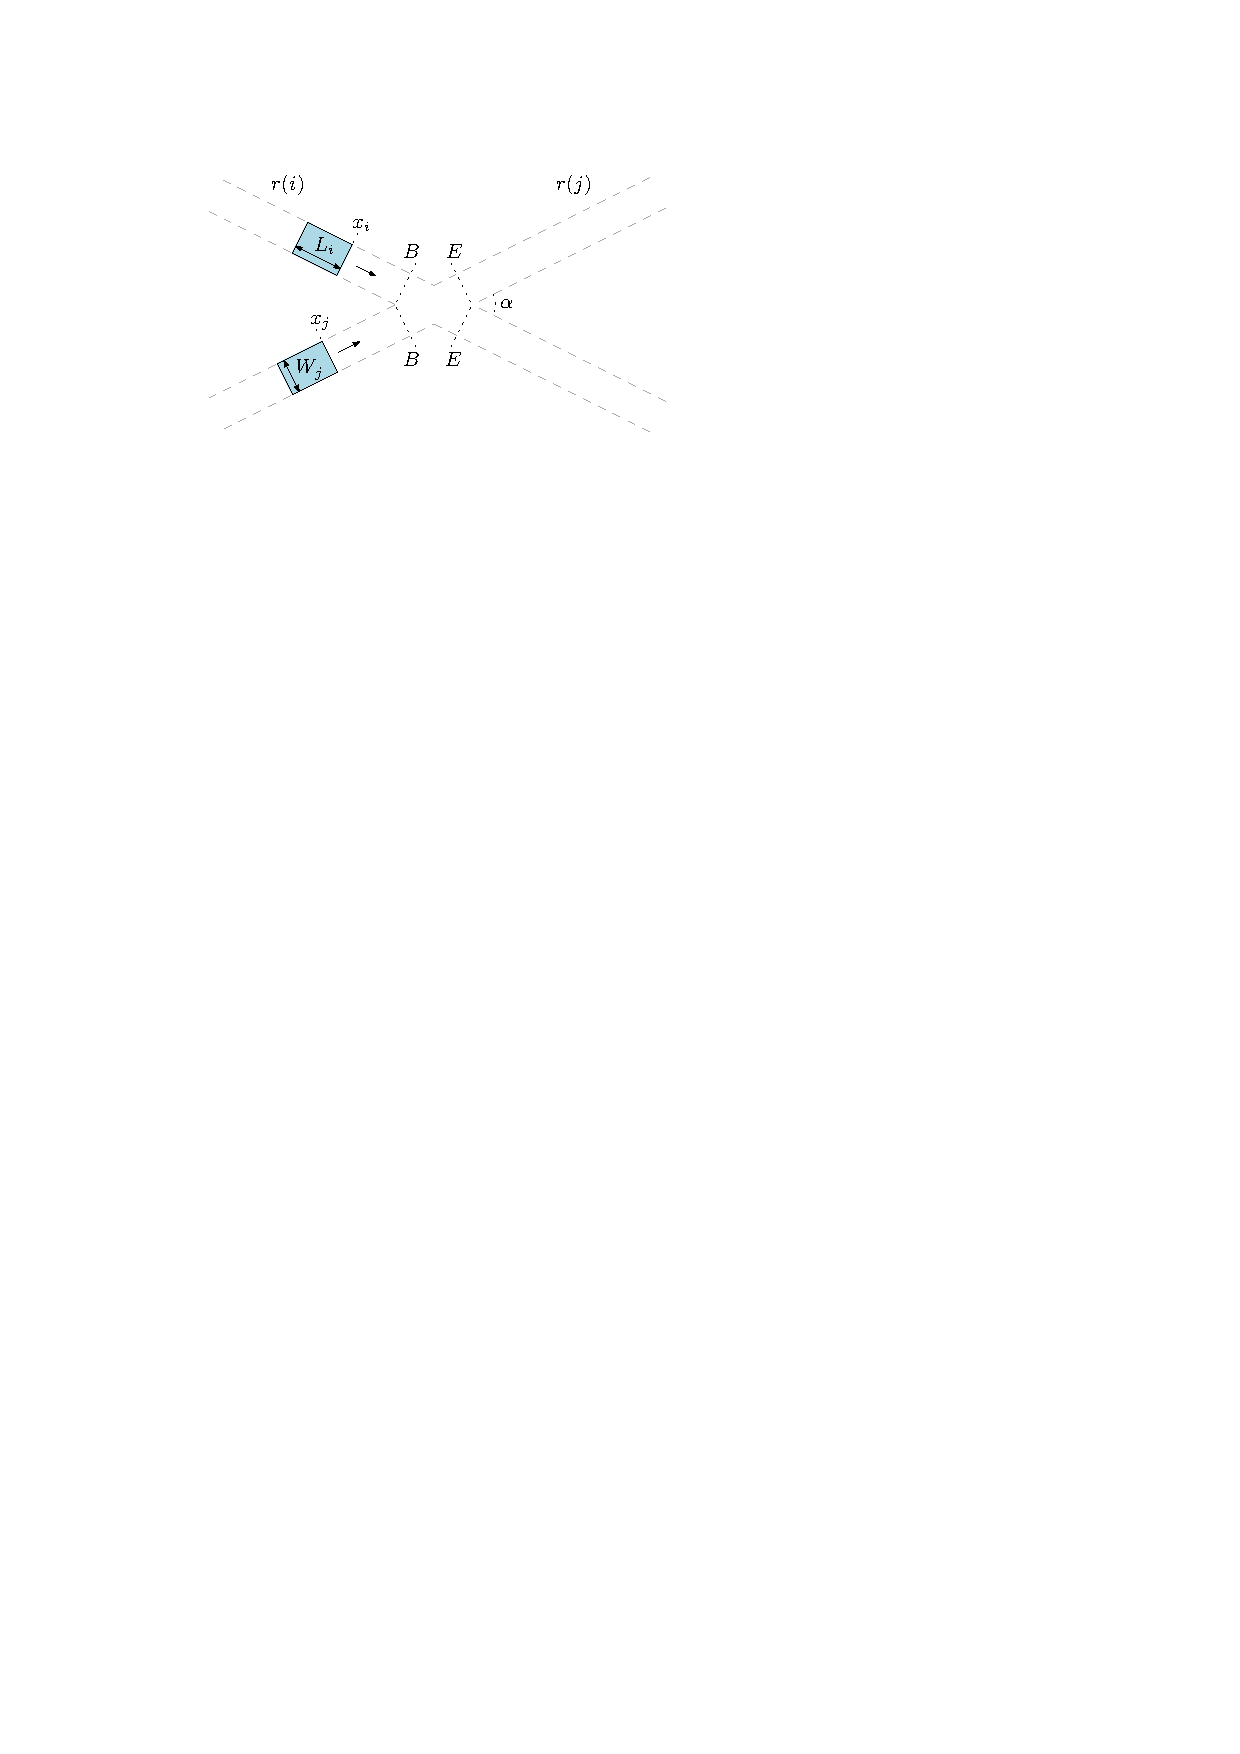
\includegraphics[scale=1]{figures/intersection-non-axis-aligned-annotated}
  \caption{Example of two vehicle routes intersecting at some angle $\alpha$. The
    indicated positions $x_{i} = B$ and $x_{i} = E$ for each vehicle $i$ are
    chosen such that whenever the vehicle position $x_{i}$ satisfies either
    $x_{i} \leq B$ or $x_{i} - L_{i} \geq E$, then the intersection area is not
    occupied by this vehicle at all and the other vehicle can take any position
    without causing a collision.}%
  \label{fig:intersection-non-axis-aligned}
\end{figure}


\section{Intersection model}

We model each vehicle $i$ in the plane as some rigid body $\mathcal{B}_{i}$
traveling along some straight line $r(i)$, to which we will refer as the
vehicle's \emph{route}.
%
We will assume that vehicles always stay on their route and thus do not make
turning maneuvers.
%
Therefore, the longitudinal position of a vehicle along its route can be
represented by some scalar $x_{i} \in \mathbb{R}$.
%
For simplicity, we use a rectangular vehicle geometry, so each $\mathcal{B}_{i}$
is a translated rectangle of width $W_{i}$ and length $L_{i}$. Therefore, we
will write $\mathcal{B}_{i}(x_{i})$ to denote the corresponding translated rigid
body in the plane, where $x_{i}$ corresponds to the location of the front
bumper; the rear bumper position is then $x_{i} - L_{i}$.
%
We allow multiple routes to cross in a single point. Of course, this causes some
joint vehicle positions to be invalid, because they would correspond to
collisions.
%
Before we allow arbitrary numbers of vehicles to have the same route, we briefly
investigate the valid configurations of two vehicles, each on its own route.

% motivates the perpendicular assumption
\paragraph{Valid configurations.}

Consider two routes intersecting at some angle $\alpha$, as illustrated in
Figure~\ref{fig:intersection-non-axis-aligned}, each with a single vehicle on
it. Let these vehicles be denoted as $i$ and $j$.
%
We can try to characterize the set $\mathcal{X}_{ij} \subset \mathbb{R}^{2}$ of
feasible configurations $(x_{i}, x_{j})$ for which these two vehicles are not in
a collision, in the sense that their corresponding translated rigid bodies do
not intersect.
%
In general, this set can thus simply be defined as
\begin{align}
  \label{eq:3}
  \mathcal{X}_{ij} := \{ (x_{i}, x_{j}) \in \mathbb{R}^{2} : \mathcal{B}_{i}(x_{i}) \cap \mathcal{B}_{j}(x_{j}) = \varnothing \} .
\end{align}
%
However, it is often easier to take the opposite perspective, by characterizing the set of conflicting configurations $\mathcal{X}_{ij}^{C}$.
\comment{Nice, ``C'' for conflict and for complement!}

% discuss rectangular subset of configuration space
%
In the situation with two routes, we fix two reference positions $B$ and $E$ on
each route, delimiting the intersection area as shown in
Figure~\ref{fig:intersection-non-axis-aligned}.
%
These positions are chosen such that whenever $x_{i} \leq B$ or
$x_{i} - L_{i} \geq E$, it is clear that vehicle $i$ does not occupy the intersection
at all, so the other vehicle $j$ is free to take any position
$x_{j} \in \mathbb{R}$.
%
Thus, we obtain the following conservative approximation of the set of conflicting
configurations:
\begin{align}\label{eq:conf-space-approx}
  [B,E + L_{i}] \times [B, E + L_{j}] \supseteq \mathcal{X}_{ij}^{C} .
\end{align}
Of course, the set of feasible configurations is generally a little larger and
depends on the angle $\alpha$ of intersection, as illustrated by the three examples
in Figure~\ref{fig:intersection-config-spaces}.
%
In case of the third example, where the intersections make a right angle
$\alpha = \pi/2$, it can be shown that there is actually equality in~\eqref{eq:conf-space-approx}.

To keep the presentation simple, we will make the following assumption: all
vehicles share the same vehicle geometry, i.e, $L_{i} \equiv L$ and
$W_{i} \equiv W$. As a shorthand of the vehicle positions that correspond to
occupying the intersection area, we will write $\mathcal{E} := [B, E + L]$.
%
This enables us to model any number of intersecting routes, as long as we can
assume that $\mathcal{E}$ provides a conservative approximation of all
intersection-occupying vehicle positions.

\begin{figure}
  \centering
  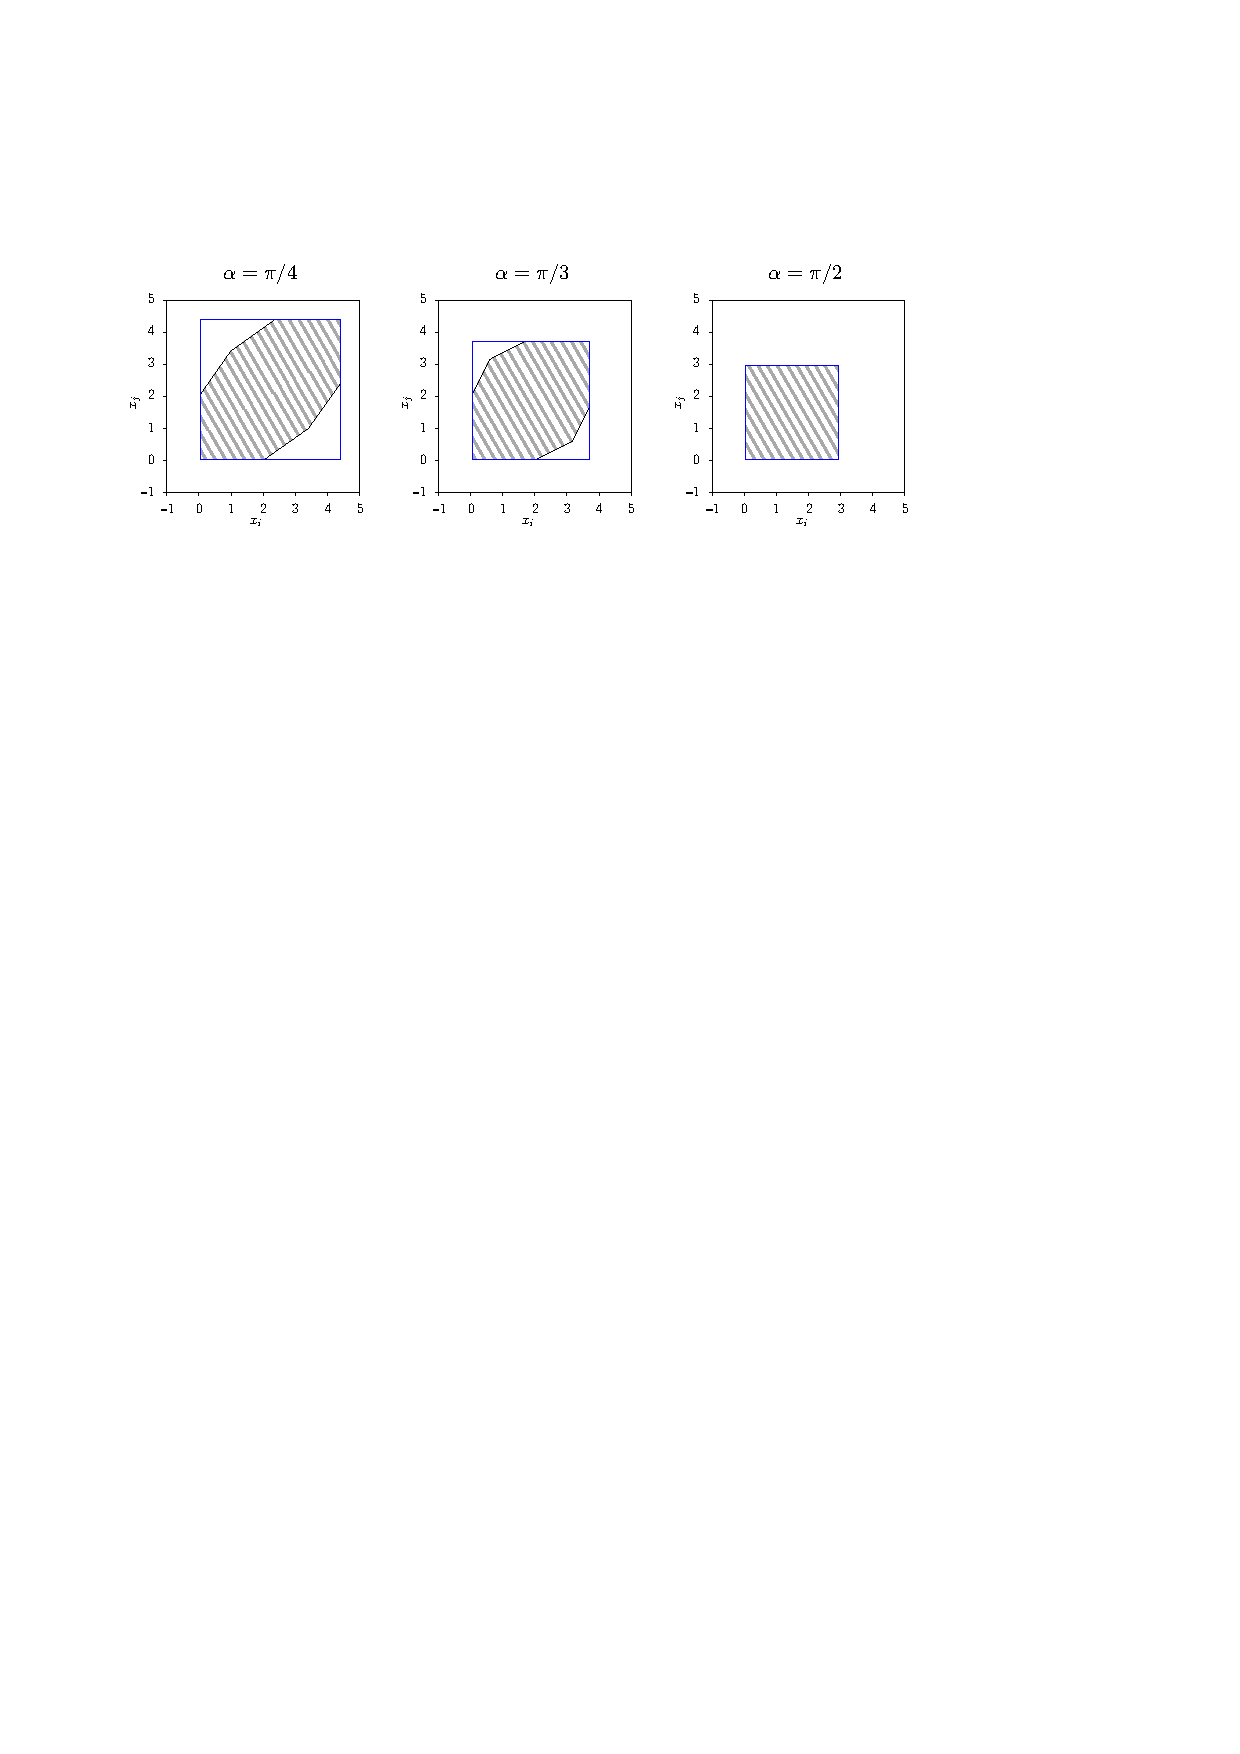
\includegraphics[scale=1]{figures/intersection-config-spaces}
  \caption{For three different intersection angles and fixed vehicle dimenions
    $W_{i} = W_{j} = 1$ and $L_{i} = L_{j} = 2$, we plotted the region
    $\mathcal{X}_{ij}^{C}$ in configuration space corresponding to collisions as
    the area marked in grey. The blue square regions correspond to the
    approximation of the collision area using~\eqref{eq:conf-space-approx}. Because we assume a
    rectangular vehicle geometry, these figures are relatively straightforward
    to compute, which we briefly explain in
    Appendix~\ref{app:configuration-space}.}%
  \label{fig:intersection-config-spaces}
\end{figure}

% collision-avoidance in routes
% \paragraph{Multiple vehicles.}
Let us now proceed to arbitrary numbers of vehicles. We will use the following
notation for identifying routes and vehicles.
%
Let the routes be identified by indices $\mathcal{R}$. Let $n_{r}$ denote the
number of vehicles following route $r$, then the set of vehicle indices is
defined as
\begin{align}
  \mathcal{N} = \{ (r, k) : k \in \{1, \dots, n_{r}\}, r \in \mathcal{R}\} .
\end{align}
Occasionally, we will also write $\mathcal{N}_{r}$ to denote the set of vehicles
on route $r$. Given vehicle index $i = (r, k) \in \mathcal{N}$, we use the
notation $r(i) = r$ and $k(i) = k$.

% conjunctions (vehicle following)
In order to maintain a safe distance between consecutive vehicle on the same
route, vehicles need to satisfy the \textit{safe headway constraints}
\begin{align}
  \label{eq:follow_constraints}
  x_{i} - x_{j} \geq L ,
\end{align}
at all times, for all pairs of indices $i, j \in \mathcal{N}$ such that
$r(i) = r(j)$ and $k(i) + 1 = k(j)$. Let $\mathcal{C}$ denote the set of all
such ordered pairs of indices. Note that these constraints restrict vehicles
from overtaking each other, so their initial relative order is always
maintained. In other words, $(i,j) \in \mathcal{C}$ means that $i$ crosses the
intersection before $j$.

% disjunctions (conflicts)
Similarly, let $\mathcal{D}$ denote the set of \emph{conflicts}, which are all
(unordered) pairs of vehicles $i, j \in \mathcal{N}$ on different routes
$r(i) \neq r(j)$.
%
Recall that we introduced $\mathcal{E}$ to denote the interval of positions for
which some vehicle is said to \emph{occupy} the intersection. Then, for each conflict
$\{i,j\}$, we impose at all times the \emph{safe crossing constraints}
\begin{align}
  \label{eq:2}
  (x_{i}, x_{j}) \notin \mathcal{E}^{2} .
\end{align}

\paragraph{Trajectory optimization.}
Next, we introduce the motion dynamics of the vehicles, so let $x_{i}(t)$ denote
the position of vehicle $i$ at time $t$.
%
Let $\dot{x}_{i}$ and $\ddot{x}_{i}$ denote its speed and acceleration,
respectively, then we consider the bounds
\begin{subequations}\label{eq:vehicle-dynamics}
\begin{align}
  \dot{x}_{i}(t) \in [\hspace{0.05em} 0, \bar{v}]  , \label{eq:speed-constr} \\
  \ddot{x}_{i}(t) \in [\hspace{0.1em} -\omega, \bar{\omega} \, ] ,
\end{align}
\end{subequations}
for some positive $\bar{v}, \omega, \bar{\omega} > 0$.
%
Given a pair of initial position and velocity $s_{i} = (x_{i}^{0}, v_{i}^{0})$,
we write $x_{i} \in D(s_{i})$ if and only if the trajectory $x_{i}$ has
$(x_{i}(0), \dot{x}_{i}(0)) = s_{i}$ and satisfies~\eqref{eq:vehicle-dynamics}.
%
The acceleration is often considered to be the main input under control, so that
vehicle position is indirectly determined by integrating twice. For this reason,
this simple vehicle dynamics model is commonly refered to as the \emph{double integrator}
model in optimal control literature.

We now present some different ways of measuring how desirable some individual
vehicle trajectory $x_{i}(t)$ is, which we will do in terms of defining a cost
functional $J(x_{i})$ that we aim to minimize.
%
First of all, we could use the absolute value of the acceleration as a proxy for
energy consumption, by setting
\begin{align}
  J(x_{i}) = \int_{0}^{t_{f}} |\ddot{x}_{i}(t)| \diff t .
\end{align}
%
\comment{There are nice physics arguments why one proxy is prefered over the
  other, but we just ignore this.}
%
As another example involving energy, consider the cost functional
\begin{align}\label{eq:energy-objective}
  J(x_{i}) = \int_{0}^{t_{f}} {\ddot{x}_{i}(t)}^{2} + {(v_{d} - \dot{x}_{i}(t))}^{2} \diff t ,
\end{align}
where $v_{d} > 0$ is some reference velocity. This objective can be roughly
interpreted as trying to maintain a velocity close to $v_{d}$, while
simultaneously minimizing the square of acceleration as proxy of energy
consumption.
%
Alternatively, if we do not want to take into account energy consumption, but
instead want to promote throughput of the overall system, a natural choice is to
consider the negative cumulative distance
\begin{align}\label{eq:haste-objective}
  J(x_{i}) = - \int_{0}^{t_{f}} x_{i}(t) \diff t .
\end{align}
We will also call the minimization of this cost functional the \emph{haste objective},
which can be interpreted as trying to have each vehicle reach the intersection
as fast as possible.

Given some $J(\cdot)$, we can now conclude our model description by defining the
general trajectory optimization problem.
%
Given the pairs of initial vehicle positions and velocities
$s := \{s_{i} = (x_{i}^{0}, v_{i}^{0}) : i \in \mathcal{N} \}$ and some final
simulation time $t_{f} > 0$, we consider the problem
%
\comment{T for ``trajectory''.}
\begin{alignat}{3}\label{eq:single-trajectory-optimization}
  T(s) := \min_{x} \;\, & \sum_{i \in \mathcal{N}} J(x_{i}) \tag{T} \\
  \text{such that } \; & x_{i} \in D(s_{i}) && \quad \text{ for all } i \in \mathcal{N} , \tag{T.1} \label{eq:T1} \\
  % \text{such that } \; & (x_{i}(0), \dot{x}_{i}(0)) = (x_{i}^{0}, v_{i}^{0}) && \quad \text{ for all } i \in \mathcal{N} ; \nonumber \\
           % \omit\rlap{and for all $t \in [0,t_{f}]$:} \notag \\
           % & \dot{x}_{i}(t) \in [0, \bar{v}]  && \quad \text{ for all } i \in \mathcal{N} , \nonumber \\
           % & \ddot{x}_{i}(t) \in [{-\omega}, \bar{\omega}] && \quad \text{ for all } i \in \mathcal{N} , \nonumber \\
           & x_{i}(t) - x_{j}(t) \geq L && \quad \text{ for all } (i,j) \in \mathcal{C} , \tag{T.2} \label{eq:T2}\\
           & (x_{i}(t), x_{j}(t)) \notin \mathcal{E}^{2} && \quad\text{ for all } \{i, j\} \in \mathcal{D} . \tag{T.3} \label{eq:T3}
\end{alignat}

Problem~\eqref{eq:single-trajectory-optimization} is non-convex in some sense;
recall that the set of feasible configurations $\mathcal{X}_{ij}$ for two
vehicles is already non-convex.\comment{I say ``roughly speaking'', because I am
  not sure personally what this even means precisely. My guess is that the set
  of feasible function, which is a subset of some underlying vector space of
  functions, is convex.}
%
An interpretation of this non-convexity is that we must decide which of the
vehicles crosses the intersection first.
%
The next section will discuss ways of dealing with this non-convexity.

\begin{remark}\label{rem:state-constraints}
  Note that the variables in~\eqref{eq:single-trajectory-optimization} represent
  continuous-time trajectories, so it is an infinite-dimensional optimization
  problem.
  %
  This kind of problems is typically studied in the framework of optimal control theory.
  %
  In this context, the joint position $x = \{x_{i} : i \in \mathcal{N}\}$ is
  refered to as the \emph{state} of the system and
  $\ddot{x} = \{\ddot{x}_{i} : i \in \mathcal{N} \}$ as the \emph{control}.
  %
  A more canonical way of writing such problems assumes $x \in \mathbb{R}^{n}$ and
  $u \in \mathbb{R}^{m}$ satisfy the dynamics
  \begin{align}\label{eq:general-dynamics}
    \dot{x} = f(t, x, u) , \quad x(t_{0}) = x_{0} , \quad u \in U \subset \mathbb{R}^{m},
  \end{align}
  for some initial state $x_{0}$ and time $t_{0}$. Given some final time $t_{f}$,
  the goal is to minimize some running cost $L$ and some terminal cost $K$ in the
  following way:
  \begin{subequations}\label{eq:opt-control}
  \begin{align}
    \min_{x} \; & \int_{t_{0}}^{t_{f}} L(t, x(t), u(t)) \diff t + K(t_{f}, x_{f}) , \\
      \textnormal{such that } \, &\eqref{eq:general-dynamics} \textnormal{ holds, } \\
                    & h(x) = 0 , \label{eq:state-constr-eq} \\
                    & g(x) \leq 0 , \label{eq:state-constr-ineq}
  \end{align}
  \end{subequations}
  with some functions $h : \mathbb{R}^{n} \rightarrow \mathbb{R}^{p}$ and
  $g : \mathbb{R}^{n} \rightarrow \mathbb{R}^{q}$ encoding the so-called state
  constraints. Functions $f, g, h$ are usually assumed to posses certain
  regularity or smoothness properties.
  %
  There are general methods to analyze optimal solutions
  of~\eqref{eq:opt-control}, most notably the necessary conditions given by the
  maximum principle of Pontryagin.
  %
  However, the occurence of state constraints~\eqref{eq:state-constr-eq}
  and~\eqref{eq:state-constr-ineq} make such analysis notoriously difficult and
  remains an area of ongoing research.
  %
  For our current problem, note that our collision-avoidance
  constraints~\eqref{eq:T2} and~\eqref{eq:T3}, as well as the implicit speed
  constraint~\eqref{eq:speed-constr} in~\eqref{eq:T1}, are of the
  type~\eqref{eq:state-constr-ineq}.
\end{remark}


\paragraph{Feasibility.}

Note that the existence feasible trajectories in~\eqref{eq:single-trajectory-optimization} generally depends on the
initial state $s$ of vehicles in some non-trivial manner.%
\footnote{Note that we will precisely characterize the feasibility of trajectories for a
related problem setting in Chapter~\ref{chap:network}.
%
However, the main difference is that the analysis there will not assume initial vehicle
states are given, but rather the times at which vehicles enter the system.}
%
To give a rough idea, we derive some simple sufficient conditions.
% feasibility assumption
We exclude initial collisions at time $t=0$ by requiring
\begin{align}\label{eq:room-assumption}
 x_{i}^{0} - x_{j}^{0} > L \quad \text{ for all } \quad  (i,j) \in \mathcal{C} .
\end{align}
%
% full acc/dec times and distances
%
Next, observe that the bounds on speed and acceleration imply that it takes at
least $1/\omega$ time to fully decelerate from full speed, during which the vehicle
has traveled a distance of $1/(2\omega)$. For a full acceleration from a stop, we
obtain the same expressions, but with $\omega$ replaced by $\bar{\omega}$.
%
Therefore, by assuming that each vehicle starts at full speed $v_{i}^{0} = 1$
and by imposing a minimum distance to the start of the intersection
\begin{align}
  x_{(r,1)}^{0} < B - 1/(2\omega) - 1/(2\bar{\omega}),
\end{align}
for each first vehicle on every route
$r \in \mathcal{R}$, we ensure that there is enough room for all vehicles to
come to a full stop. Even further, there is still enough distance for a full
acceleration to reach full speed while crossing the intersection.


\section{From joint optimization to bilevel decomposition}

To tackle the trajectory optimization
problem~\eqref{eq:single-trajectory-optimization}, we first employ a numerical
method known as \emph{direct transcription}.
%
The key idea is to reformulate the continuous-time optimal control
problem---which is infinite-dimensional---as a finite-dimensional nonlinear
optimization problem by discretizing the time horizon into a grid.
%
At each grid point, the state and control inputs of every vehicle become
decision variables. The vehicle dynamics and the safety requirements, i.e., the
headway and collision-avoidance constraints, can then be imposed directly in
terms of these decisions variables.
%
This approach allows us to capture the full structure of the problem while
making it accessible to modern nonlinear optimization solvers.
%
In what follows, we describe in detail how this general approach can be applied
to our current problem and illustrate its use by solving some examples for two
different cost functionals.

\paragraph{Joint optimization.}
We start by defining a uniform discretization grid. Let $K$ denote the number of
discrete time steps and let $\Delta t$ denote the time step size, then we define
\begin{align}
  \mathbb{T} := \{0, \Delta t, \dots, K \Delta t\} .
\end{align}
%
For each vehicle $i$, we use $x_{i}(t), v_{i}(t)$ and $u_{i}(t)$ to denote,
respectively, the decision variables for position, speed and acceleration.
%
First of all, we impose the initial conditions by simply adding the constraints
$x_{i}(0) = x_{i}^{0}$ and $v_{i}(0) = v_{i}^{0}$ for each $i \in \mathcal{N}$.
%
Using the forward Euler integration scheme, we further relate these three
quantities by adding the constraints
\begin{subequations}
\begin{align}
  x_{i}(t + \Delta t) = x_{i}(t) + v_{i}(t) \Delta t , \\
  v_{i}(t + \Delta t) = v_{i}(t) + u_{i}(t) \Delta t ,
\end{align}
\end{subequations}
for each $t \in \mathbb{T} \setminus \{K\Delta t\}$ and $i \in \mathcal{N}$. Moreover, we directly include
the inequalities $0 \leq v_{i}(t) \leq \bar{v}$ and
${-\omega} \leq u_{i}(t) \leq \bar{\omega}$ to model the vehicle dynamics.
%
For each pair of consecutive vehicles $(i, j) \in \mathcal{C}$ on the same route,
the safe headway constraints can simply be added as
\begin{align}
  x_{i}(t) - x_{j}(t) \geq L \quad \text{ for each } t \in \mathbb{T}.
\end{align}

Encoding of the safe crossing constraints needs some additional attention.
%
Following the approach in~\cite{hultApproximateSolutionOptimal2015}, these disjunctive constraints can be formulated
using the common big-$M$ method with binary decision variables. For each vehicle
$i \in \mathcal{N}$, we introduce two binary decision variables
$\delta_{i}(t), \gamma_{i}(t) \in \{ 0, 1 \}$ and for each conflict $\{i, j\} \in \mathcal{D}$ and
time step $t \in \mathbb{T}$, we introduce the following constraints:
\begin{subequations}\label{eq:collision-avoidance-binary-encoding}
  \begin{align}
  x_{i}(t) &\leq B + \delta_{i}(t) M , \label{eq:order-constr-1} \\
  \quad x_{i}(t) &\geq E + L - \gamma_{i}(t) M , \label{eq:order-constr-2} \\
  & \hspace{-3.8em} \delta_{i}(t) + \delta_{j}(t) + \gamma_{i}(t) + \gamma_{j}(t) \leq 3 , \label{eq:order-constr-3}
  \end{align}
\end{subequations}
where $M$ is some sufficiently large number.
%
The idea behind this encoding is as follows.
%
First, observe that setting $\delta_{i}(t) $ can be thought of as
\emph{deactivating}~\eqref{eq:order-constr-1}, since $M$ is chosen sufficiently
large such that the inequality is trivially true. Analogously, setting
$\gamma_{i}(t) = 1$ deactivates~\eqref{eq:order-constr-2}.
%
Hence, the constraint~\eqref{eq:order-constr-3} can be interpreted as limiting
the number of deactivations to three, which is equivalent to requiring at least
one of the following four inequalities to hold:
\begin{align}
  x_{i}(t) \leq B, \quad x_{j}(t) \leq B , \quad
  x_{i}(t) \geq E + L, \quad x_{j}(t) \geq E + L ,
\end{align}
which means that vehicles $i$ and $j$ cannot both occupy the intersection at the
same time $t$.

In general, the resulting transcribed optimization problem is a mixed-integer
nonlinear program. We consider the two energy-based criteria for a small problem
with five vehicles, for which the optimal trajectories are shown in Figure~\ref{fig:direct_transcription_example}.
\comment{Optionally include running time analysis to motivate the need for fast
  approximations.}

\begin{remark}
  We used the forward Euler integration scheme for sake of a simple
  presentation. However, note that in practice we most likely want to use a more
  numerically stable method like a higher-order Runge-Kutta scheme or by means
  of some spline interpolation technique (collocation). We refer
  to~\cite{Ch10Trajectory} for a light introduction of trajectory optimization
  and~\cite{kellyIntroductionTrajectoryOptimization2017} for a tutorial on the
  direct collocation method, which also contains a concise overview of different
  numerical methods in (ibid., Section 9).
\end{remark}


\begin{figure}
  \centering
  \begin{minipage}{0.76\textwidth}
  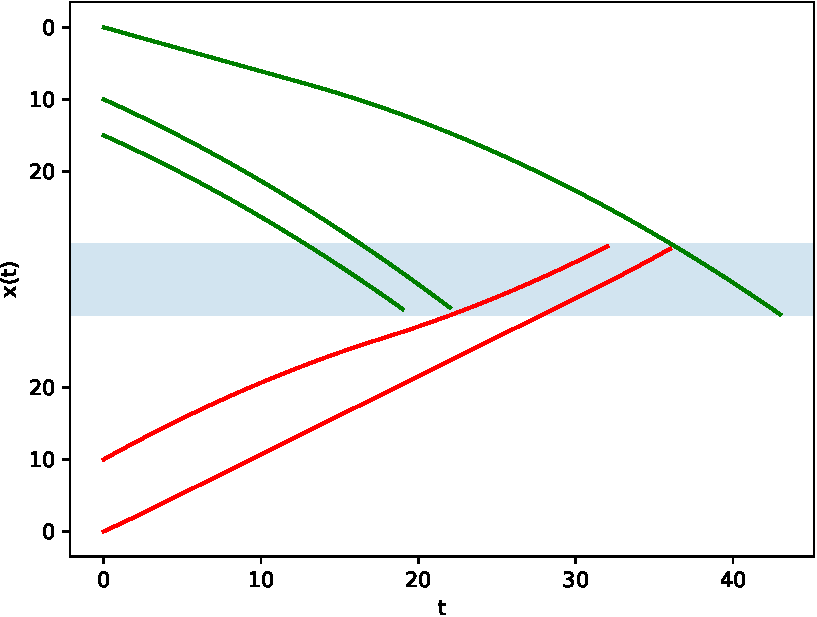
\includegraphics[width=0.9\textwidth]{figures/single/trajectories_general.pdf}%
  \end{minipage}
  \begin{minipage}{0.23\textwidth}
  \vspace*{-1em}
  \begin{tabular}{ c c c }
    $i$ & $x_{i}^{0}$ & $v_{i}^{0}$ \\[0.2em]
    \hline\\[-1em]
    {\color{red}(1,3)} &  0 & 1.0 \\
    {\color{red}(1,2)} & 10 & 1.0 \\
    {\color{red}(1,1)} & 15 & 1.0 \\
    {\color{blue}(2,1)} & 10 & 0.8 \\
    {\color{blue}(2,2)} &  0 & 0.0
  \end{tabular}
  \end{minipage}
  \caption{Example of optimal trajectories for two objectives, obtained using
    the direct transcription method with parameters
    $L = 5, \, \mathcal{E} = [20, 30], \, \bar{v} = 1, \, \omega = \bar{\omega} = 0.1, \, v_{d} = 0.6, \; T=50, \, \Delta t = 1$
    and initial conditions as given in the table. The y-axis is split such that
    the top part corresponds to route $1$ and the bottom to route $2$ and the
    trajectories are inverted accordingly and drawn with separate colors. The
    interval of intersection occupying positions $\mathcal{E}$ is drawn as a
    shaded region. We stop drawing a trajectory after it leaves the
    intersection.}%
  \label{fig:direct_transcription_example}
\end{figure}

\paragraph{Bilevel decomposition.}

After applying the transcription method above, the safe crossing constraints of
each conflict are imposed for every time step, requiring in total $2T$ binary
variables.
%
Therefore, there is some kind of redundancy in this encoding, because the
decision to be made is, in principle, a single binary decision for each
conflict, deciding which of the two vehicle crosses the intersection first.
%
However, note that such an encoding would require decision variables for the
time of entry into and exit out of the intersection for each vehicle.
%
This insight is the key to decomposing the problem into an upper-level and a set
of lower-level problems.
%
Roughly speaking, the upper-level problem optimizes the time slots during which
vehicles occupy the intersection, while the lower-level problems produce optimal
safe trajectories that respect these time slots.
%
\comment{c.f. Benders' decomposition}
%
The following presentation and notation is adapted
from~\cite{hultApproximateSolutionOptimal2015}.
%
Throughout the following discussion, we assume the system parameters
$(L,B,E, \bar{v}, \omega, \bar{\omega}, t_{f})$ to be fixed.

Given some feasible trajectory $x_{i} \in D(s_{i})$ for a single vehicle $i$, we
define its (earliest) \emph{entry} time and (earliest) \emph{exit} time,
respectively, to be
%
\begin{subequations}
\begin{alignat}{2}
  \tau(x_{i}) &:=& \, \min &\{ t \in [0, t_{f}] : x_{i}(t) = B \} , \\
  \xi(x_{i}) &:=& \, \min &\{ t \in [0, t_{f}] : x_{i}(t) = E + L \} .
\end{alignat}
\end{subequations}
Note that the sets in the definition are closed, because $x_{i}$ is continuous,
but they may be empty. Therefore, we use the convention that
``$\min \varnothing = \infty$'', such that $\tau(x_{i}) = \infty$ whenever $x_{i}$
does not reach the intersection at all and, analogously, we have
$\xi(x_{i}) = \infty$ whenever the end of the intersection is never reached.
Furthermore, using the convention that $[\infty, \infty] = \varnothing$, observe
that $\tau(x_{i})$ and $\xi(x_{i})$ determine the times
$t \in [\tau(x_{i}), \xi(x_{i})]$ during which vehicle $i$ occupies the
intersection.
%
Recall the encoding of the collision constraints using binary variables
in~\eqref{eq:collision-avoidance-binary-encoding}.
%
Similarly, observe that the
collision-avoidance constraints
\begin{align}
  (x_{i}(t), x_{j}(t)) \notin \mathcal{E}^{2} \quad \text{ for all } \{i,j\} \in \mathcal{D}
\end{align}
are completely equivalent to the constraints
\begin{align}\label{eq:disjoint-occupancy}
  [\tau(x_{i}), \xi(x_{i})] \cap [\tau(x_{j}), \xi(x_{j})] = \varnothing \quad \text{ for all } \{i,j\} \in \mathcal{D} .
\end{align}
%
The main idea of the decomposition is to make these entry and exit times
concrete decision variables of the upper-level problem.
%
Hence, for each vehicle $i$, we introduce a decision variable $y_{i}$ for the
time of entry and a variable $z_{i}$ for the time of exit.
%
When the occupancy time slots $\{[y_{i}, z_{i}] : i \in \mathcal{N}\}$ are fixed
and satisfy~\eqref{eq:disjoint-occupancy}, the trajectory optimization problem
essentially reduces to solving a separate lower-level problem for each route.

In order to make this more precise, let us introduce some shorthand notation for
collections of parameters and variables pertaining to a single route.
%
Let $\mathcal{N}_{r} \subset \mathcal{N}$ be all vehicle indices of route $r$.
We write $s_{r} := \{(x_{i}^{0}, v_{i}^{0}) : i \in \mathcal{N}_{r} \}$ to
denote the corresponding initial conditions and we write
$x_{r} := \{x_{i} : i \in \mathcal{N}_{r} \}$ as a shorthand for a set of
trajectories on route $r$. \comment{For me personally, the subscript r is not a
  problem. Alternatively, we could use boldface notation to emphasize that s_r,
  x_r, y_r, z_r are actually sets/collections/vectors (set is best, because
  there is no inherent order, because we already have indices).}
%
Consider some route $r \in \mathcal{R}$ with local initial conditions $s_{r}$ and
suppose we are given some fixed local occupancy time slots as determined by
$y_{r} := \{y_{i} : i \in \mathcal{N}_{r}\}$ and
$z_{r} := \{z_{i} : i \in \mathcal{N}_{r}\}$, then we define the lower-level \emph{route planning problem}
%
\begin{alignat}{3}\label{eq:lower-level}
  F(y_{r},z_{r}, s_{r}) := \min_{x_{r}} \;\, & \sum_{i \in \mathcal{N}_{r}} J(x_{i}) \tag{L} \\
  \text{s.t. } \; & x_{i} \in D(s_{i})  && \quad \text{ for all } i \in \mathcal{N}_{r} , \tag{L.1} \\
  & x_{i}(t) - x_{j}(t) \geq L && \quad \text{ for all } (i,j) \in \mathcal{C} \cap \mathcal{N}_{r} , \tag{L.2} \\
  & x_{i}(y_i) = B  && \quad \text{ for all } i \in \mathcal{N}_{r} , \tag{L.3} \label{eq:L3} \\
  & x_{i}(z_{i}) = E + L  && \quad \text{ for all } i \in \mathcal{N}_{r} . \tag{L.4} \label{eq:L4}
\end{alignat}
%
Note that the feasibility of this problem depends on the initial states as well
as the choice of occupancy time slots. Therefore, given initial states $s_{r}$,
we write $(y_{r}, z_{r}) \in \mathcal{T}(s_{r})$ to denote the set of occupancy
time slots that allow a feasible solution.

The upper-level problem is now to find a set of occupancy timeslots
satisfying~\eqref{eq:disjoint-occupancy}, such that the lower-level problem for
each route is feasible. Let $s = \{s_{r} : r \in \mathcal{R} \}$ denote the set of
global initial states for all routes and write $y = \{y_{r} : r \in \mathcal{R} \}$ and
$z = \{y_{z} : r \in \mathcal{R}\}$ to denote a set of global occupancy time
slots, then we define the upper-level \textit{occupancy scheduling problem}
%
\comment{U for ``upper''.}
\begin{alignat}{2}\label{eq:upper-level}
  U(s) := \min_{y, z} \quad & \sum_{r \in \mathcal{R}} F({y}_{r}, {z}_{r}, s_{r}) \tag{U} \\
  \text{ s.t. } \quad & [y_{i},z_{i}] \cap [y_{j},z_{j}] = \varnothing & \quad \text{ for all } \{i, j\} \in \mathcal{D} , \tag{U.1} \\
                            & ({y}_{r}, {z}_{r}) \in \mathcal{T}(s_{r}) & \text{ for all } r \in \mathcal{R} . \tag{U.2}
\end{alignat}

Without further assumptions, problem~\eqref{eq:upper-level} is not necessarily
equivalent to the original problem~\eqref{eq:single-trajectory-optimization}.
%
A major issue lies in the fact that some feasible solution $x$ of~\eqref{eq:single-trajectory-optimization} does not
need to cross the intersection at all, i.e., it is not guaranteed that $\tau(x)$
and $\xi(x)$ are finite for $x$.
%
To illustrate such situations, consider the following (pathological) example.
\begin{eg}
  Suppose we have a single vehicle on each route, both having initial speed
  $v_{i}^{0} = \bar{v}$ and some initial distance $x_{i}^{0}$ satisfying the
  assumption~\eqref{eq:room-assumption}, such that each vehicle can perform a
  full deceleration ($\ddot{x}_{i} = \omega$) and come to a stop somewhere
  before the start of the intersection, so that $x_{i}(1/\omega) < B$. Consider
  the cost functional
  \begin{align}
    J(x_{i}) = \int_{0}^{t_{f}} x_{i}(t) \diff t ,
  \end{align}
  then it is easily seen that the optimal solution is to have both vehicles
  decelerate immediately as just described.
  %
  In contrast, any solution $x'$ obtained by solving~\eqref{eq:upper-level} will
  cross the intersection sometime and thus has a strictly larger objective
  value.
\end{eg}

There are different ways to resolve this issue. A possible approach is to
require that all vehicle trajectories satisfy\footnote{The authors
  of~\cite{hultApproximateSolutionOptimal2015} refer to this as ``strongly
  output monotone''.}
\begin{align}\label{eq:strongly-output-monotone}
  \dot{x}_{i}(t) \geq \epsilon \quad \text{ for all } t \in [0, t_{f}] ,
\end{align}
for some $\epsilon > 0$, which ensures
existance of $\tau(x_{i})$ and $\xi(x_{i})$, assuming $t_{f}$ is sufficiently large.
%
With this assumption, for a single vehicle per route and a cost functional of
the form
\begin{align}
  J(x_{i}) = \int_{0}^{t_{f}} \Lambda(x_{i}(\tau), \dot{x}_{i}(\tau), \ddot{x}_{i}(\tau)) \diff \tau ,
\end{align}
for some convex and quadratic function $\Lambda(x,v,u)$, it has been argued that~\eqref{eq:single-trajectory-optimization}
and~\eqref{eq:upper-level} are equivalent~\cite[Theorem 1]{hultTechnicalReportApproximate}.
%
Their argument relies on showing that the lower-level has a unique solution.
However, as we will illustrate shortly hereafter, there are interesting problem
settings for which this does not hold.
%
Instead of assumption~\eqref{eq:strongly-output-monotone}, we will just
explicitly restrict the set feasible trajectories to cross the intersection by
focusing on the problem variant
\begin{alignat}{3}\label{eq:single-trajectory-optimization-variant}
  T^{*}(s) := \min_{x} \;\, & \sum_{i \in \mathcal{N}} J(x_{i}) \tag{T*} \\
  \text{s.t. } \; & x_{i} \in D(s_{i}) && \quad \text{ for all } i \in \mathcal{N} , \nonumber \\
           & x_{i}(t) - x_{j}(t) \geq L && \quad \text{ for all } (i,j) \in \mathcal{C} , \nonumber \\
           & (x_{i}(t), x_{j}(t)) \notin \mathcal{E}^{2} && \quad\text{ for all } \{i, j\} \in \mathcal{D} , \nonumber \\
           & \tau(x_{i}) < \infty && \quad \text{ for all } i \in \mathcal{N} , \tag{T*.4} \label{eq:T4*} \\
           & \xi(x_{i}) < \infty && \quad  \text{ for all } i \in \mathcal{N} . \tag{T*.5} \label{eq:T5*}
\end{alignat}

Another issue that needs attention is the possibility
of~\eqref{eq:single-trajectory-optimization} not having an optimal solutions,
even if feasible (see~\cite[Section 4.5]{liberzonCalculusVariationsOptimal}).

\begin{theorem}
  \note{ Assume problem~\eqref{eq:single-trajectory-optimization-variant} is
    feasible and an optimal solution exists, then this problem is equivalent to
    the decomposed problem~\eqref{eq:upper-level}.}
\end{theorem}
\begin{proof}
  \note{
  Every $(y,z)$ has one or more solutions $x$.
  %
  Every $x$ has a single unique $(y,z)$.}
\end{proof}

\begin{remark}
  The constraints~\eqref{eq:L3},~\eqref{eq:L4},~\eqref{eq:T4*}
  and~\eqref{eq:T5*} are state constraints of a different type than those
  discussed in Remark~\ref{rem:state-constraints}. Namely, $g(x(t)) \leq 0$ is
  imposed for all times $t \in [t_{0}, t_{f}]$.
  %
  However, the constraint $x_{i}(y_{i}) = B$ only holds at some prespecified
  intermediate time $y_{i} \in [t_{0}, t_{f}]$ and may be interpreted as some
  kind of ``checkpoints''.
  %
  This situation is not typically considered in the literature, but it is
  possible to reduce the problem into a canonical form that only has such
  equality constraints at the endpoints of the time interval, i.e.,
  $x(t_{0}) = x_{0}$ and $x(t_{f}) = x_{f}$,
  see~\cite{dmitrukMaximumPrincipleOptimal2011}.
  %
  Whenever $t_{f} < \infty$, the constraints $\tau(x_{i}) < \infty$ and
  $\xi(x_{i}) < \infty$ together can be replaced by the equivalent endpoint
  constraint $x_{i}(t_{f}) \geq E + L$.
\end{remark}


\paragraph{Solving the decomposition.}

When the decomposition is sound, i.e., if both problems are indeed equivalent,
it provides a good basis for developing alternative solution methods. However,
the decomposed problem is not necessarily easier to solve.
%
In general, the difficulty of solving~\eqref{eq:upper-level} lies in the fact
that $F$ is a non-trivial function of the occupancy time slots and
$\mathcal{T}(s_{r})$ is not easily characterizable, e.g., as a system of
inequalities.

For a single vehicle per route, so $(y_{r}, z_{r}) \equiv (y_{i},z_{i})$, the
approach taken in~\cite{hultApproximateSolutionOptimal2015} is to approximate
both these objects as follows: they fit a quadratic function for
$F(y_{i}, z_{i}, s_{i})$ and they approximate the set of feasible occupancy
slots by considering the polyhedral subset
\begin{align}
  \{ (y, z) : y \in [T_{i}^{l},T_{i}^{h}], \; l_{i}(y) \leq z \leq u_{i}(y) \} \subseteq \mathcal{T}(s_{i}) ,
\end{align}
for some earliest entry time $T_{i}^{l}$ and latest entry time $T_{i}^{h}$ and
strictly increasing affine functions $u_{i}(\cdot)$ and $l_{i}(\cdot)$. They
provide conditions that guarantee that solutions computed using this
approximation method are feasible.
%
To circumvent the need for such approximations, we will make some additional
assumptions, which allows us to focus on the combinatorial part of the problem
in the next section.

\paragraph{More assumptions.}

We will introduce a trajectory cost criterion that acts as a proxy of the amount
of delay experienced by vehicles, by defining $J(x_{i}) = \tau(x_{i})$.
%
This choice makes the problem significantly simpler,
because we avoid the need to approximate $F$, because we simply have
\begin{alignat}{2}
  U(s) = \min_{y, z} \quad & \sum_{i \in \mathcal{N}} y_{i} \nonumber \\
  \text{ s.t. } \quad & [y_{i},z_{i}] \cap [y_{j},z_{j}] = \varnothing && \quad \text{ for all } \{i, j\} \in \mathcal{D} , \nonumber \\
                           & ({y}_{r}, {z}_{r}) \in \mathcal{T}(s_{r}) && \quad \text{ for all } r \in \mathcal{R} , \nonumber
\end{alignat}
which means that the only remaining difficulty is how to deal with feasibility
of the lower-level problem.
%
Moreover, we assume that all vehicles start at full speed $v_{i}^{0} = \bar{v}$
\note{and introduce the additional constraint that vehicles must enter the
  intersection at full speed, i.e., we add the constraint
  $\dot{x}_{i}(\tau(x_{i})) = \bar{v}$ to~\eqref{eq:single-trajectory-optimization-variant} and $\dot{x}_{i}(y_{i}) = \bar{v}$
  to~\eqref{eq:lower-level}. [do we need this?]} Let the resulting problems
variants be denoted (T**) and (L**), respectively \comment{I know, this is not
  the prettiest; I will think about a different way of writing this.}

Under these assumptions, the set of feasible parameters $\mathcal{T}(s_{r})$ is
now easier to characterize.
%
First of all, because every $x_{i}$ in a set of feasible trajectories for~(L**)
satisfies $x_{i}(y_{i}) = \bar{v}$, observe that we can let each vehicle
continue at full speed across the intersection, which takes exactly
$\sigma := (B-E)/\bar{v}$ time, so we can always set
\begin{align*}
  z_{i} = y_{i} + \sigma, \; \text{ for all } i \in \mathcal{N} .
\end{align*}
%
With this choice, observe that $\rho := L / \bar{v}$ is such that
$x_{i}(y_i + \rho) = x(y_{i}) + L = B + L$, which is the time after which the
next vehicle from the same route can enter the intersection, so we will refer to
$\rho$ as the \textit{processing time}.
%
Since $z_{i}$ is not involved in $J$, this means we only have to care about finding
\begin{align}
  \label{eq:1}
  \mathcal{T}_{y}(s_{r}) := \{ y_{r} : (y_{r}, y_{r} + \sigma) \in \mathcal{T}(s_{r}) \} ,
\end{align}
where $y_{r} + \sigma$ is to be understood as
$\{y_{i} + \sigma : i \in \mathcal{N}_{r}\}$.
%
It can be shown that $y_{r} \in \mathcal{T}_{y}(s_{r})$ holds if and only if
\begin{align*}
  a_{i} \leq y_i & \quad \text{ for all } i \in \mathcal{N}_{r} , \\
  y_i + \rho \leq y_j & \quad \text{ for all } (i,j) \in \mathcal{C} \cap \mathcal{N}_{r} ,
\end{align*}
where $a_{i} := (B - x_{i}^{0}) / \bar{v}$ is the earliest time at which vehicle
$i$ can enter the intersection.
%
A rigorous proof of this fact is outside the scope of the current chapter, but
we note that the analysis is very similar to that of
Chapter~\ref{chap:network}. \comment{It would be nice to include a
  retrospective proof in that later chapter, but note that there is a subtle
  difference: whereas we provide initial *positions* here, we will later
  consider initial *entry times*.}

To conclude this section, the stated assumptions mean that problem (U**) reduces
to the following \textit{crossing time scheduling} problem
\begin{subequations}
\begin{alignat}{2}\label{eq:crossing_time_scheduling}
  \min_{y} \quad & \sum_{i \in \mathcal{N}} y_i \tag{C} \\
  \text{ s.t. } \quad & a_{i} \leq y_i  && \quad \text{ for all } i \in \mathcal{N} , \tag{C.1} \\
                    & y_i + \rho \leq y_{j}  && \quad \text{ for all } (i,j) \in \mathcal{C} \label{eq:conjunctive} , \tag{C.2} \\
                    & [y_{i}, y_i + \sigma] \cap [y_{j}, y_j + \sigma] = \varnothing && \quad \text{ for all } \{i,j\} \in \mathcal{D} \label{eq:disjunctive} \tag{C.3}.
\end{alignat}
\end{subequations}
This is a typical scheduling problem, which can for example be solved using the
mixed-integer linear programming framework after encoding the \textit{disjunctive
  constraints}~\eqref{eq:disjunctive} using the big-M technique. This methodology will be
explored in the next section.


\section{Crossing time scheduling}
\label{sec:branch-and-cut}

The conclusion of the previous section is that, under certain assumptions, the
trajectory optimization problem~\eqref{eq:single-trajectory-optimization}
reduces to a scheduling problem~\eqref{eq:crossing_time_scheduling} of finding a
crossing time schedule $y$ that determines the time of crossing for each vehicle
in the sytem.
%
Correponding trajectories can be computed relatively efficiently for each route separately using a direct transcription method.
%
Hence, in the remainder of this chapter and the next chapter, we will focus on
solving the crossing time scheduling problem.
%
First, we show how to leverage the branch-and-cut framework by
formulating~\eqref{eq:crossing_time_scheduling} as a Mixed-Integer Linear
Program (MILP) and defining three types of cutting planes. We investigate the
computational complexity of this approach for different classes of problems in
Section~\ref{sec:runtime}. As an illustration of an alternative solution approach, Section~\ref{sec:local_search}
briefly discusses a local search heuristic.
%
The next chapter will discuss methods to learn heuristics using a data-driven
methodology.

\subsection{Branch-and-cut}

To formulate the crossing time scheduling problem as a MILP, we rewrite the
disjunctive constraints using the well-known big-M method by introducing a
binary decision variable $\gamma_{ij}$ for every disjunctive pair
$\{i, j\} \in \mathcal{D}$.
%
To avoid redundant variables, we first impose some arbitrary ordering of the
disjunctive pairs by defining
\begin{align*}
  \bar{\mathcal{D}} = \{ (i,j) : \{i,j\} \in \mathcal{D}, \; r(i) < r(j) \} ,
\end{align*}
such that for every $(i,j) \in \bar{\mathcal{D}}$, setting $\gamma_{ij} = 0$
corresponds to choosing disjunction $i \rightarrow j$ and $\gamma_{ij} = 1$ corresponds to
$j \rightarrow i$. This yields the following MILP formulation
%
\begin{align*}
  \min_{y} \quad & \sum_{i \in \mathcal{N}} y_{i} - a_{i} & \\
  \text{s.t.} \quad & a_{i} \leq y_{i} , & \text{ for all } i \in \mathcal{N} , \\
  & y_{i} + \rho \leq y_{j} , & \text{ for all } (i,j) \in \mathcal{C} , \\
  & y_{i} + \sigma \leq y_{j} + \gamma_{ij}M , & \text{ for all } (i,j) \in \bar{\mathcal{D}} , \\
  & y_{j} + \sigma \leq y_{i} + (1 - \gamma_{ij})M , & \text{ for all } (i,j) \in \bar{\mathcal{D}} , \\
  & \gamma_{ij} \in \{0, 1\} , & \text{ for all } (i,j) \in \bar{\mathcal{D}} ,
\end{align*}
where $M > 0$ is some sufficiently large number. This problem can be solved by
any off-the-shelf MILP solving software. Next, we will discuss three types of
cutting planes that can be added to this formulation, which we hope improves the
solving time.

\paragraph{Cutting planes.}
Consider some disjunctive arc $(i,j) \in \bar{\mathcal{D}}$. Let
$\mathit{pred}(i)$ denote the set of indices of vehicles that arrive no later
than $i$ on route $r(i)$. Alternatively, we could say
these are all the vehicles from which there is a path of conjunctive arcs to
$i$. Similarly, let $\mathit{succ}(j)$ denote the set of indices of vehicles
that arrive no later than $j$ on route $r(j)$.
%
Now suppose $\gamma_{ij} = 0$, so the direction of the arc is $i \rightarrow j$,
then any feasible solution must also satisfy
\begin{align*}
  p \rightarrow q \equiv \gamma_{pq} = 0 \; \text{ for all } \; p \in \mathit{pred}(i), \; q \in \mathit{succ}(j) .
\end{align*}
Written in terms of the disjunctive variables, this gives the following cutting
planes
\begin{align*}
  \sum_{\substack{p \in \mathit{pred}(i)\\ q \in \mathit{succ}(j)}} \gamma_{pq} \leq \gamma_{ij} M ,
\end{align*}
for every conflict $(i,j) \in \bar{\mathcal{D}}$. We refer to these as
the \textit{transitive cutting planes}.

% Under the condition that $\rho_{i} = \rho$ and $\sigma_{i} = \sigma > \rho$ for all $i \in \mathcal{N}$,

Apart from the redundancy that stems from the way the conflicts are encoded, we
will now study some less obvious structure in the problem.
%
Let us briefly consider some trivial examples to establish some better intuition
for the problem.

\begin{eg}
  Consider the trivial problem with two routes and a single vehicle per route.
  When both vehicles have the same earliest arrival time $a_{i} = a$, the order
  in which they cross the intersection does not matter for the final objective,
  which is $\sigma$. When either of the vehicles has a strictly earlier release
  date, then it is obvious that this vehicle must go first in the optimal
  schedule.
\end{eg}
%
\begin{eg}
  \label{example2}
  Consider two routes having one and two vehicles, respectively. Instead of
  $(1,1), (2,1), (2,2)$, we will use the labels $1, 2, 3$ to keep notation
  clear. We are interested in how the earliest crossing times influence the
  order of the vehicles in an optimal schedule. We set $a_{1} = 0$, without loss
  of generality, and assume that $a_{3} = a_{2} + \rho$. Suppose
  $a_{1} = a_{2}$, then we see that the order $2, 3, 1$ is optimal, which
  resembles some sort of ``longest chain first'' rule. Now suppose that
  $a_{1} < a_{2}$. For $a_{2} \geq a_{1} + \rho + \sigma$, the sequence
  $1, 2, 3$ is simply optimal. For $a_{2} < a_{1} + \rho + \sigma$, we compare
  the sequence $1, 2, 3$ with $2, 3, 1$, which are illustrated in
  Figure~\ref{fig:example2}. The first has
  $\sum_{i} y_{i} = (\rho+\sigma) + (\rho+\sigma+\rho) = 3\rho + 2\sigma$,
  while the second sequence has
  $\sum_{i} y_{i} = a_{2} + (a_{2} + \rho) + (a_{2} + \rho + \rho + \sigma) = 3 a_{2} + 3\rho + \sigma$.
  Therefore, we conclude that the second sequence is optimal if and only if
  \begin{align}
    \label{eq:before-condition}
    a_{2} \leq \sigma/3 ,
  \end{align}
  which roughly means that the ``longest chain first'' rule becomes optimal
  whenever the release dates are ``close enough''.
\end{eg}
%
\begin{figure}[t]
  \centering
  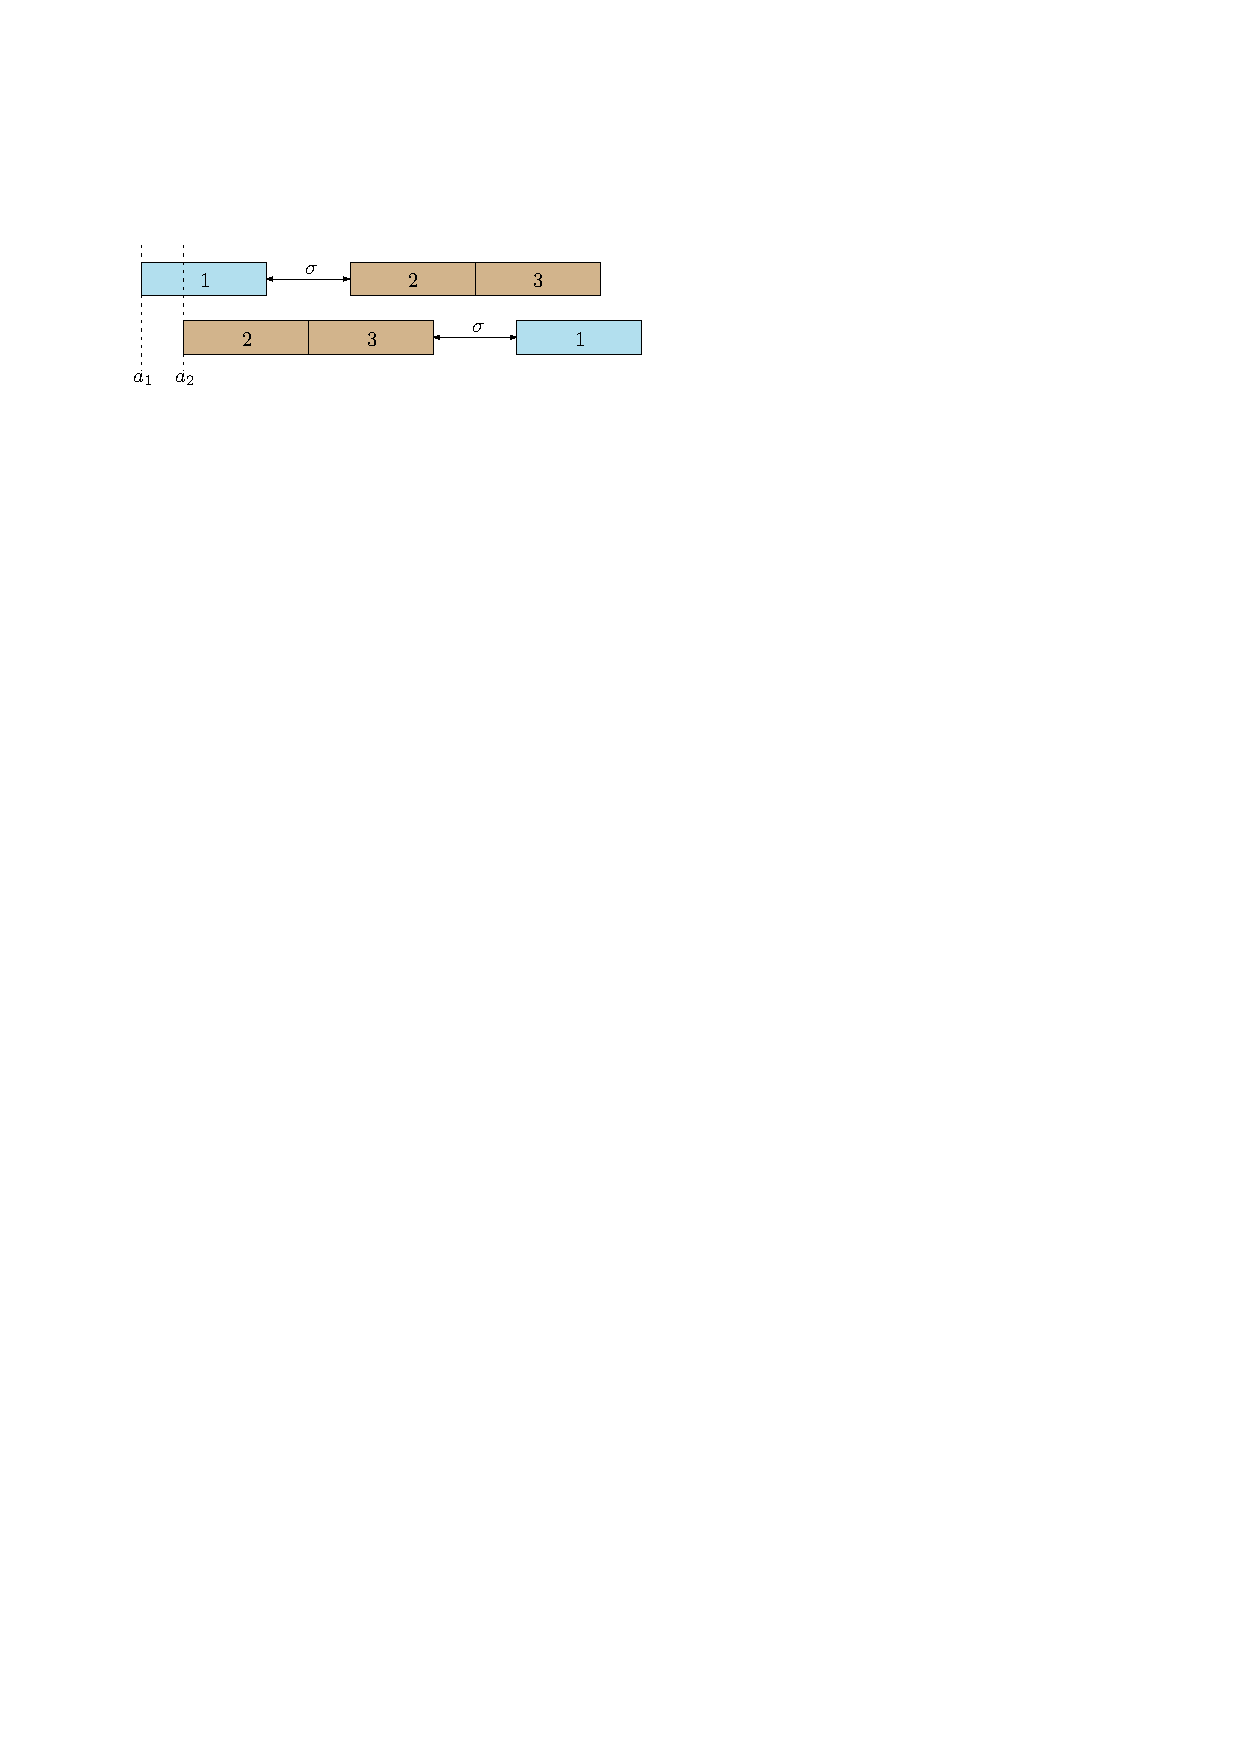
\includegraphics[width=0.55\textwidth]{figures/single/123.pdf}
  \caption{Illustration of the two possible sequences of vehicles in
    Example~\ref{example2}.}
  \label{fig:example2}
\end{figure}

In the previous example, we see that it does not make sense to schedule vehicle
1 between vehicles 2 and 3, because that would add unnecessary $\sigma$ time. This
raises the question whether splitting such \textit{platoons} of vehicles is ever
necessary to achieve an optimal schedule. Let us first give a precise definition
of this notion, before slightly generalizing the example above.
%
\begin{define}
  A sequence of consecutive vehicles $(r, l+1), (r, l+2), \dots, (r, l+n)$ from
  some route $r$ is called a \textit{platoon} of size $n$ if and only if
  \begin{align*}
  a_{(r,k)} + \rho = r_{(r, k+1)}  \quad \quad \text{ for all } l < k < l + n.
  \end{align*}
 We say that the platoon is \textit{split}
  in some schedule $y$, if
  \begin{align*}
  y_{(r, k)} + \rho < y_{(r, k + 1)} \quad \quad \text{ for some } l < k < l + n.
  \end{align*}
\end{define}
%
\begin{eg}
  \label{example3}
  Suppose we have two routes $\mathcal{R} = \{ A, B \}$, each having exactly one
  platoon, denoted as $P_{A} = ((A,1), \dots, (A,n_{A}))$,
  $P_{B} = ((B,1), \dots, (B,n_{B}))$. To simplify notation, we write
  $a_{A} = a_{(A,1)}$ and $a_{B} = a_{(B,1)}$. We assume $a_{A} = 0$, without
  loss of generality, and suppose that $n_{A} < n_{B}$ and
  $a_{A} \leq a_{B} < n_{A}\rho + \sigma$. Consider the ways the two platoons
  can merge by splitting A. Let $k$ denote the number of vehicles of platoon A
  that go before platoon B and let $\sum y_{i}(k)$ denote the corresponding
  sum of crossing times. See Figure~\ref{fig:example3} for an illustration of the
  situation in case of $a_{A} = a_{B}$. For $0 < k \leq n_{A}$, we have
  \begin{align*}
    \sum_{i \in \mathcal{N}} y_{i} (k) = \max\{ \sigma, a_{B} - k\rho\} (n_{B} + n_{A} - k) + \sigma (n_{A} - k) + \sum_{j=1}^{n_{A}+n_{B}} (j-1) \rho ,
  \end{align*}
  so when platoon A goes completely before platoon B, we get
  \begin{align}
    \sum_{i \in \mathcal{N}} y_{i} (n_{A}) = \sigma n_{B} + \sum_{j=1}^{n_{A}+n_{B}} (j-1) \rho ,
    \label{eq:A-before-B}
  \end{align}
  since $\max\{ \sigma, a_{B} - n_{A} \rho \} = \sigma$ by the assumption on
  $a_{B}$. It is easily seen that we have $\sum y_{i}(k) > \sum y_{i} (n_{A})$
  for $0 < k < n_{A}$, so in other words, if we decide to put at least one
  vehicle of platoon A before platoon B, it is always better to put all of them
  in front. As we will see next, this principle holds more generally.

  For $k=0$, so when we schedule platoon A completly after platoon B, the total
  completion time becomes
  \begin{align*}
    \sum_{i \in \mathcal{N}} y_{i} (0) = a_{B} (n_{A} + n_{B}) + \sigma n_{A} + \sum_{j=1}^{n_{A}+n_{B}} (j-1) .
  \end{align*}
  Comparing this to~\eqref{eq:A-before-B}, we conclude that placing B in front
  is optimal whenever
  \begin{align*}
    a_{B} \leq (n_{B} - n_{A}) \sigma / (n_{A} + n_{B}) ,
  \end{align*}
  which directly generalizes the condition~\eqref{eq:before-condition} that we
  derived for the case with $n_{A} = 1$ and $n_{B} = 2$.
\end{eg}

\begin{figure}
  \centering
  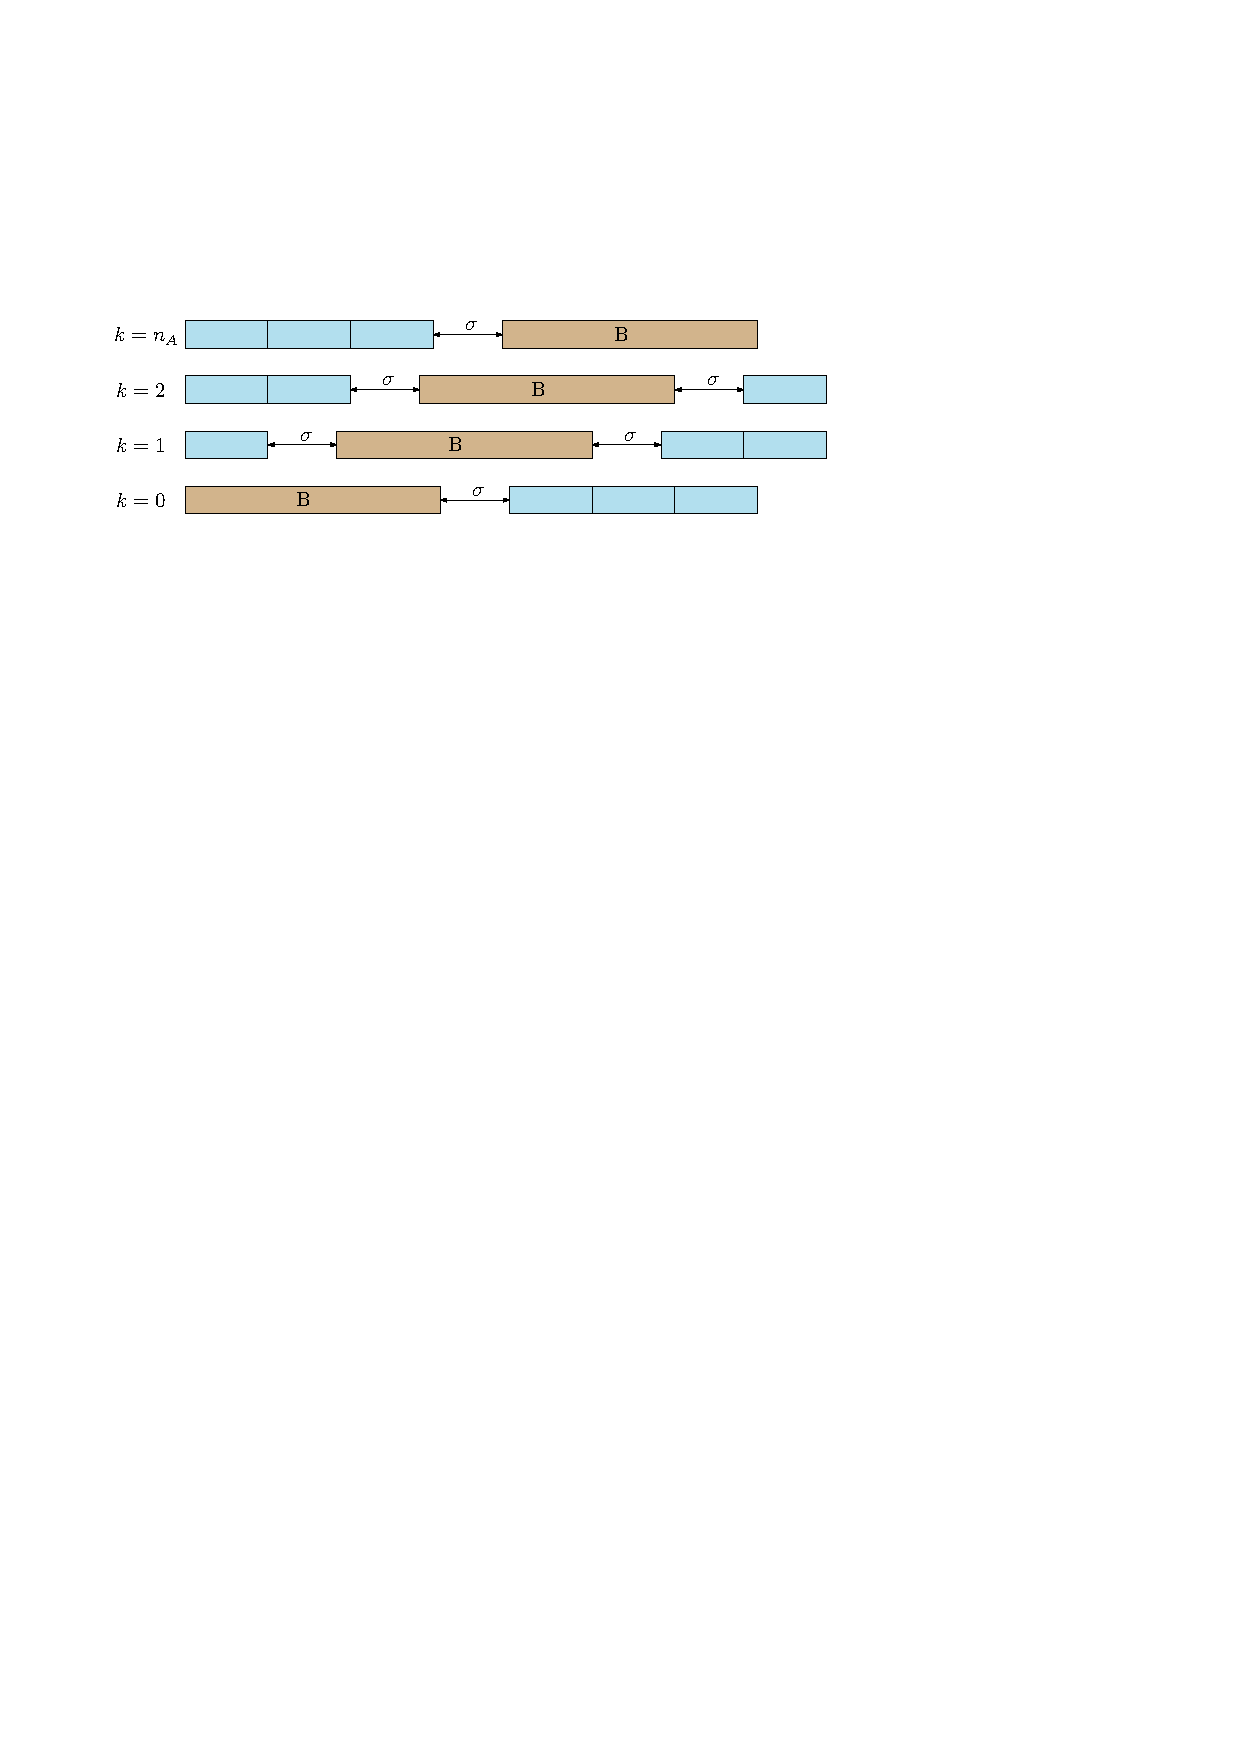
\includegraphics[scale=1]{figures/single/platoons.pdf}
  \caption{Illustration of different ways to split platoon A, regarding
    Example~\ref{example3}, assuming that $a_{A} = a_{B}$ with $n_{A} = 3$ and
    some arbitrary $n_{B}$.}
  \label{fig:example3}
\end{figure}

The example shows that, when we decide to put one vehicle of a platoon before
another platoon, it is always better to put the whole platoon in front. In other
words, whenever a vehicle can be scheduled immediately after its predecessor,
this should happen in any optimal schedule, as stated by the following result,
for which we provide a proof in Appendix~\ref{app:proof}.

\begin{restatable}[Platoon Preservation~\cite{limpensOnlinePlatoonForming2023}]{theorem}{Exhaustive}\label{prop:exhaustive}
  If $y$ is an optimal schedule for~\eqref{eq:crossing_time_scheduling},
  satisfying $y_{i^{*}} + \rho \geq a_{j^{*}}$ for some $(i^{*},j^{*}) \in \mathcal{C}$, then $j^{*}$
  follows immediately after $i^{*}$, so $y_{i^{*}} + \rho = y_{j^{*}}$.
\end{restatable}

We will now use this result to define two types of additional cutting planes. In
order to model this necessary condition, we introduce for every conjunctive pair
$(i,j) \in \mathcal{C}$ a binary variable $\delta_{ij} \in \{0, 1\}$ that satisfies
\begin{align*}
  \delta_{ij} = 0 &\iff y_{i} + \rho < a_{j} , \\
  \delta_{ij} = 1 &\iff y_{i} + \rho \geq a_{j} ,
\end{align*}
which can be enforced by adding to the constraints
\begin{align*}
  y_{i} + \rho &< a_{j} + \delta_{ij}M , \\
  y_{i} + \rho &\geq a_{j} - (1 - \delta_{ij}) M .
\end{align*}
Now observe that Theorem~\ref{prop:exhaustive} applied to $(i,j)$ is modeled by the
cutting plane
\begin{align*}
  y_{i} + \rho &\geq y_{j} - (1 - \delta_{ij}) M .
\end{align*}
We refer to these cutting planes as \textit{necessary conjunctive cutting planes}.
%
Using the definition of $\delta_{ij}$, we can add more cutting planes on the
disjunctive decision variables, because whenever $\delta_{ij} = 1$, the directions of
the disjunctive arcs $i \rightarrow k$ and $j \rightarrow k$ must be the same for every other vertex
$k \in \mathcal{N}$. Therefore, consider the following constraints
\begin{align*}
  \delta_{ij} + (1 - \gamma_{ik}) + \gamma_{jk} \leq 2 , \\
  \delta_{ij} + \gamma_{ik} + (1 - \gamma_{jk}) \leq 2 ,
\end{align*}
for every $(i,j) \in \mathcal{C}$ and for every $k \in \mathcal{N}$ with $r(k) \neq r(i) = r(j)$.
We will refer to these types of cuts as the \textit{necessary disjunctive cutting planes}.

\subsection{Runtime analysis of branch-and-cut}
\label{sec:runtime}

In order to make a comparison of the relative performance of the different
cutting planes, we first define the distribution over problem instances from
which we will take samples to use as a benchmark.

For each route $r \in \mathcal{R}$, we model the sequence of earliest crossing times
$a_{r} = (a_{r1}, a_{r2}, \dots)$ as a stochastic process, to which we refer as
the \textit{arrival process}. Recall that constraints~\eqref{eq:conjunctive}
ensure a safe following distance between consecutive vehicles on the same route.
Therefore, we want the process to satisfy
\begin{align*}
  a_{(r, k)} + \rho_{(r,k)} \leq a_{(r, k + 1)} ,
\end{align*}
for all $k = 1, 2, \dots$.
%
Let the interarrival times be denoted as $X_{n}$ with cumulative distribution
function $F$ and mean $\mu$, assuming it exists. We define the arrival times
$A_{n} = A_{n-1} + X_{n} + \rho$, for $n \geq 1$ with $A_{0} = 0$.

Note that the arrival process may be interpreted as an renewal process with interarrivals
times $X_{n} + \rho$.
%
% To be precise, let $I_{t} \in \{0, 1\}$
% denote the state of the process at time $t$ and assume the process starts in
% state $I_{0} = 0$. Let $X_{1}, X_{2}, \dots$ denote the times spend in state $0$
% and let $\rho$ be the time spend in state $1$.
%
Let $N_{t}$ denote the corresponding counting process, i.e., $N_{t}$ counts the
cumulative number of arrivals up to time $t$, then by the \textit{renewal theorem}, we
obtain the \textit{limiting density} of arrivals
%
\begin{align*}
  \mathbb{E}(N_{t + h}) - \mathbb{E}(N_{t}) \rightarrow \frac{h}{\mu + \rho} \quad \text{ as } t \rightarrow \infty ,
\end{align*}
for $h > 0$. Hence, we refer to the quantity $\lambda := {(\mu + \rho)}^{-1}$ as the
average arrival intensity.

%
% Given
% some time $t>0$, define the \textit{truncation} $a_{i}(t)$ as the finite
% subsequence $(a_{i1}, \dots, a_{ik})$ of $a_{i}$ such that $a_{ik} \leq t$.
% %
% Let $f^{*}(a_{1}(t), a_{2}(t))$ denote an optimal schedule for the crossing
% time scheduling problem with arrivals $a_{1}(t)$ and $a_{2}(t)$.
% %
% Given some schedule $y$, we say that it has a \textit{schedule renewal at
%   time} $t$ whenever there are two consecutive vehicles
% $(i, j) \in \mathcal{C}$ such that $t = y(i) + \sigma < y(j)$. Let $R(y)$ denote
% the total number of such renewals in schedule $y$. Now consider the following
% limit
% \begin{align*}
%   L = \lim_{t \rightarrow \infty} R(f^{*}(a_{1}(t), a_{2}(t))) .
% \end{align*}
% Whenever $L < \infty$, we say that the system is \textit{unstable}.
% Whenever $L = \infty$, we say the system is \textit{stable}.
%
% Because there is in general no simple expression for $f^{*}$, it is not possible
% to state a necessary and sufficient condition for stability like often done for
% queueing systems. {\color{Navy}Argue that renewals do not change under $f^{*}$.}

\paragraph{Platoons.}
In order to model the natural occurence of platoons, we model the interarrival
times $X_{n}$ as a mixtures of two random variables, one with a small expected
value $\mu_{s}$ to model the gap between vehicles within the same platoon and one
with a larger expected value $\mu_{l}$ to model the gap between vehicles of
different platoons. For example, consider a mixture of two exponentials, such
that
\begin{align*}
  F(x) &= p ( 1 - e^{-x / \mu_{s}} ) + (1 - p) (1 - e^{-x / \mu_{l}}) , \\[0.2em]
  \mu &= p \mu_{s} + (1-p) \mu_{l} ,
\end{align*}
%
assuming $\mu_{s} < \mu_{l}$. Observe that the parameter $p$ determines
the average length of platoons.
%
Consider two intersecting routes, $\mathcal{R} = \{1, 2\}$, with arrival processes
$a_{1} = (a_{11}, a_{12}, \dots)$ and $a_{2} = (a_{21}, a_{22}, \dots)$, with
arrival intensities $\lambda^{(1)} = \lambda^{(2)}$.
%
We keep $\lambda_{s} = 0.5$ constant, and use
\begin{align*}
  \mu_{l}  = \frac{\mu - p \mu_{s}}{1 - p}
\end{align*}
to keep the arrival rate constant accross arrival distributions.

\paragraph{Comparison.}
We now assess which type of cutting planes yields the overall best performance.
The running time of branch-and-cut is mainly determined by the total number of
vehicles in the instance. Therefore, we consider instances with two routes and
measure the running time of branch-and-cut as a function of the number of
vehicles per route.
%
In order to keep the total computation time limited, we set a time limit of 60
seconds for solving each instance. Therefore, we should be careful when
calculating the average running time, because some observations may correspond
to the algorithm reaching the time limit, in which case the observation is said
to be \textit{censored}. Although there are statistical methods to rigorously
deal censored data, we do not need this for our purpose of picking the best type
of cutting planes.
%
Figure~\ref{fig:running_time} shows the average (censored) running time for the
three types of cutting planes. Observe that the necessary conjunctive cutting
planes seem to lower the running time the most.


\begin{figure}
  \centering
  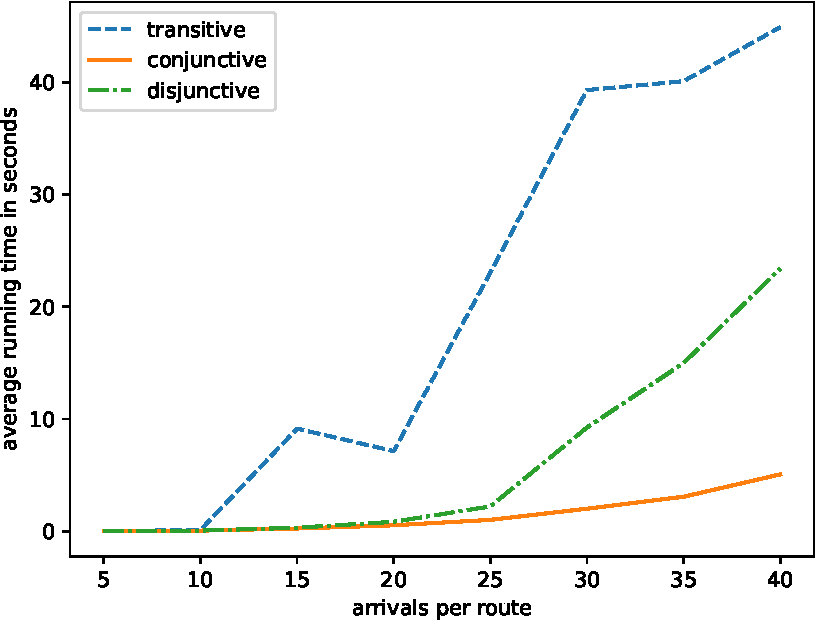
\includegraphics[width=0.6\textwidth]{data-single/running_times.pdf}
  \caption{The average running time of the branch-and-cut procedure is plotted
    as a function of the number of arriving vehicles per route, for each of the
    three indicated cutting planes. Each average is computed over $20$ problem
    instances. All instances use $\rho = 4$ and $\sigma = 1$. The arrivals of each of
    the two routes are generated using the bimodal exponential interarrival
    times with $p=0.5, \mu_{s} = 0.1, \mu_{l} = 10$. This figure clearly shows that
    the conjunctive cutting planes provide the most runtime improvement.}
  \label{fig:running_time}
\end{figure}

\subsection{Local search}
\label{sec:local_search}

Without relying on systematic search methods like branch-and-bound, we can try
to use some kind of local search. Specifically, compute a solution using one of
the methods from the previous section and then explore some \textit{neighboring
  solutions}, that we define next.

As seen in the previous sections, vehicles of the same route occur mostly in
platoons. For example, consider for example the route order
$\eta = (0, 1, 1, 0, 0, 1, 1, 1, 0, 0)$. This example has 5 platoons of consecutive
vehicles from the same route. The second platoon consists of two vehicles from
route 1.
%In general, let $P(\eta)$ denote the total number of platoons in $\eta$.
The basic idea is to make little changes in these platoons by moving vehicles at
the start and end of a platoon to the previous and next platoon of the same
route.
%
More precisely, we define the following two types of modifications to a route
order. A \textit{right-shift} modification of platoon $i$ moves the last vehicle of this
platoon to the next platoon of this route. Similarly, a \textit{left-shift} modification
of platoon $i$ moves the first vehicle of this platoon to the previous platoon
of this route.
%
We construct the neighborhood of a solution by performing every possible
right-shift and left-shift with respect to every platoon in the route order. For
illustration purposes, we have listed a full neighborhood for some example route
order in Table~\ref{tab:local_search}.

Now using this definition of a neighborhood, we must specify how the search
procedure visits these candidates.
In each of the following variants, the value of each neighbor is always computed.
%
The most straightforward way is to select the single best candidate in the
neighborhood and then continue with this as the current solution and compute its
neighborhood. This procedure can be repeated for some fixed number of times.
Alternatively, we can select the $k$ best neighboring candidates and then
compute the combined neighborhood for all of them. Then in the next step, we
again select the $k$ best candidates in this combined neighborhood and repeat.
The latter variant is generally known as \textit{beam search}.

\newcommand*{\1}{{\color{blue}1}}%
\newcommand*{\0}{{\color{red}0}}%

\begin{table}
\caption{Neighborhood of route order $\eta = (\0, \1, \1, \0, \0, \1, \1, \1, \0, \0)$.}
\label{tab:local_search}
\begin{center}
\begin{tabular}{c|c|c}
  platoon id  & left-shift & right-shift \\
  1 &  & (\1, \1, \0, \0, \0, \1, \1, \1, \0, \0) \\
  2 & (\1, \0, \1, \0, \0, \1, \1, \1, \0, \0) & (\0, \1, \0, \0, \1, \1, \1, \1, \0, \0) \\
  3 & (\0, \0, \1, \1, \0, \1, \1, \1, \0, \0) & (\0, \1, \1, \0, \1, \1, \1, \0, \0, \0) \\
  4 & (\0, \1, \1, \1, \0, \0, \1, \1, \0, \0) & (\0, \1, \1, \0, \0, \1, \1, \0, \0, \1) \\
  5 & (\0, \1, \1, \0, \0, \0, \1, \1, \1, \0) &
\end{tabular}
\end{center}
\end{table}

\section{Notes and references}

The single intersection model is mostly based on the model described
in~\cite[Chapter 3]{hultOptimizationBasedCoordination2019}.


\chapter{Optimal schedule modeling}\label{chap:single-learning}

% autoregressive modeling
Methods that are based on the branch-and-cut framework are guaranteed to find an
optimal solution, but as we illustrated in Section~\ref{sec:runtime}, their running time
generally scales very poorly with increased instance sizes. For this reason, we
are interested in developing heuristics to obtain good approximations in limited
time.
%
Specifically, we will be considering heuristics that can be formulated as
autoregressive models~\cite{tomczakDeepGenerativeModeling2024} and show how these can be tuned by using example
problem instances.

% choose disjunctive constraints -> linear program
\paragraph{Equivalent representations of schedules.}
Observe that the space of feasible solutions of~\eqref{eq:crossing_time_scheduling} can be reduced to finitely
many decisions regarding the disjunctive constraints~\eqref{eq:disjunctive}. Specifically, for each
feasible choice of the disjunctions $\mathcal{O}$, we consider the so-called
\textit{active schedule} $y$ as the unique solution to the linear program
\note{[why unique?]}
\begin{subequations}
  \label{eq:active_schedule}
\begin{align}
  \min_{y} \quad & \sum_{i \in \mathcal{N}} y_{i} \\
  \text{s.t.} \quad & a_{i} \leq y_{i} & \text{ for all } i \in \mathcal{N}, \\
           & y_{i} + \rho_{i} \leq y_{j}, & \text{ for all } (i,j) \in \mathcal{C}, \\
           & y_{i} + \sigma_{i} \leq y_{j}, & \text{ for all } (i,j) \in \mathcal{O} .
\end{align}
\end{subequations}
To see when such a selection $\mathcal{O}$ is feasible, we can think of this
linear program as a weighted directed graph on nodes $\mathcal{N}$ with
conjunctive arcs $(i,j) \in \mathcal{C}$ with weights $w(i,j) = \rho_{i}$ and
disjunctive arcs $(i,j) \in \mathcal{O}$ with weights $w(i,j) = \sigma_{i}$. Now
observe that the definition of $y$ through the linear program is equivalent to
defining $y$ through
\begin{align}
  \label{eq:y_max}
  y_{j} = \max\{ a_{j}, \max_{i \in \mathcal{N}^{-}(j)} y_i + w(i,j) \} ,
\end{align}
where $\mathcal{N}^{-}(j)$ denotes the set of in-neighbors of node $j$. It is
now easy to see that $y$ is well-defined if and only if the so-called \textit{complete disjunctive graph}
$G=(\mathcal{N}, \mathcal{C} \cup \mathcal{O})$ is acyclic.
%
When $G$ is acyclic, there is a unique topological ordering of its nodes. Hence,
any valid selection $\mathcal{O}$ of disjunctive constraints is equivalent to a
sequence $\pi$ of vehicles. It is also equivalent to a sequence $\eta$ of routes,
because the ordering of vehicles on the same route is already fixed. See
Figure~\ref{fig:disjunctive_graphs} for an example of a complete disjunctive
graph with corresponding vehicle order $\pi$ and route order $\eta$.
%
From now on, we will mainly be working with $\eta$, because it is in some sense the
simplest representation of a schedule and we write $y^{\eta}$ to denote the
corresponding induced crossing times.

\begin{figure}
  \centering
  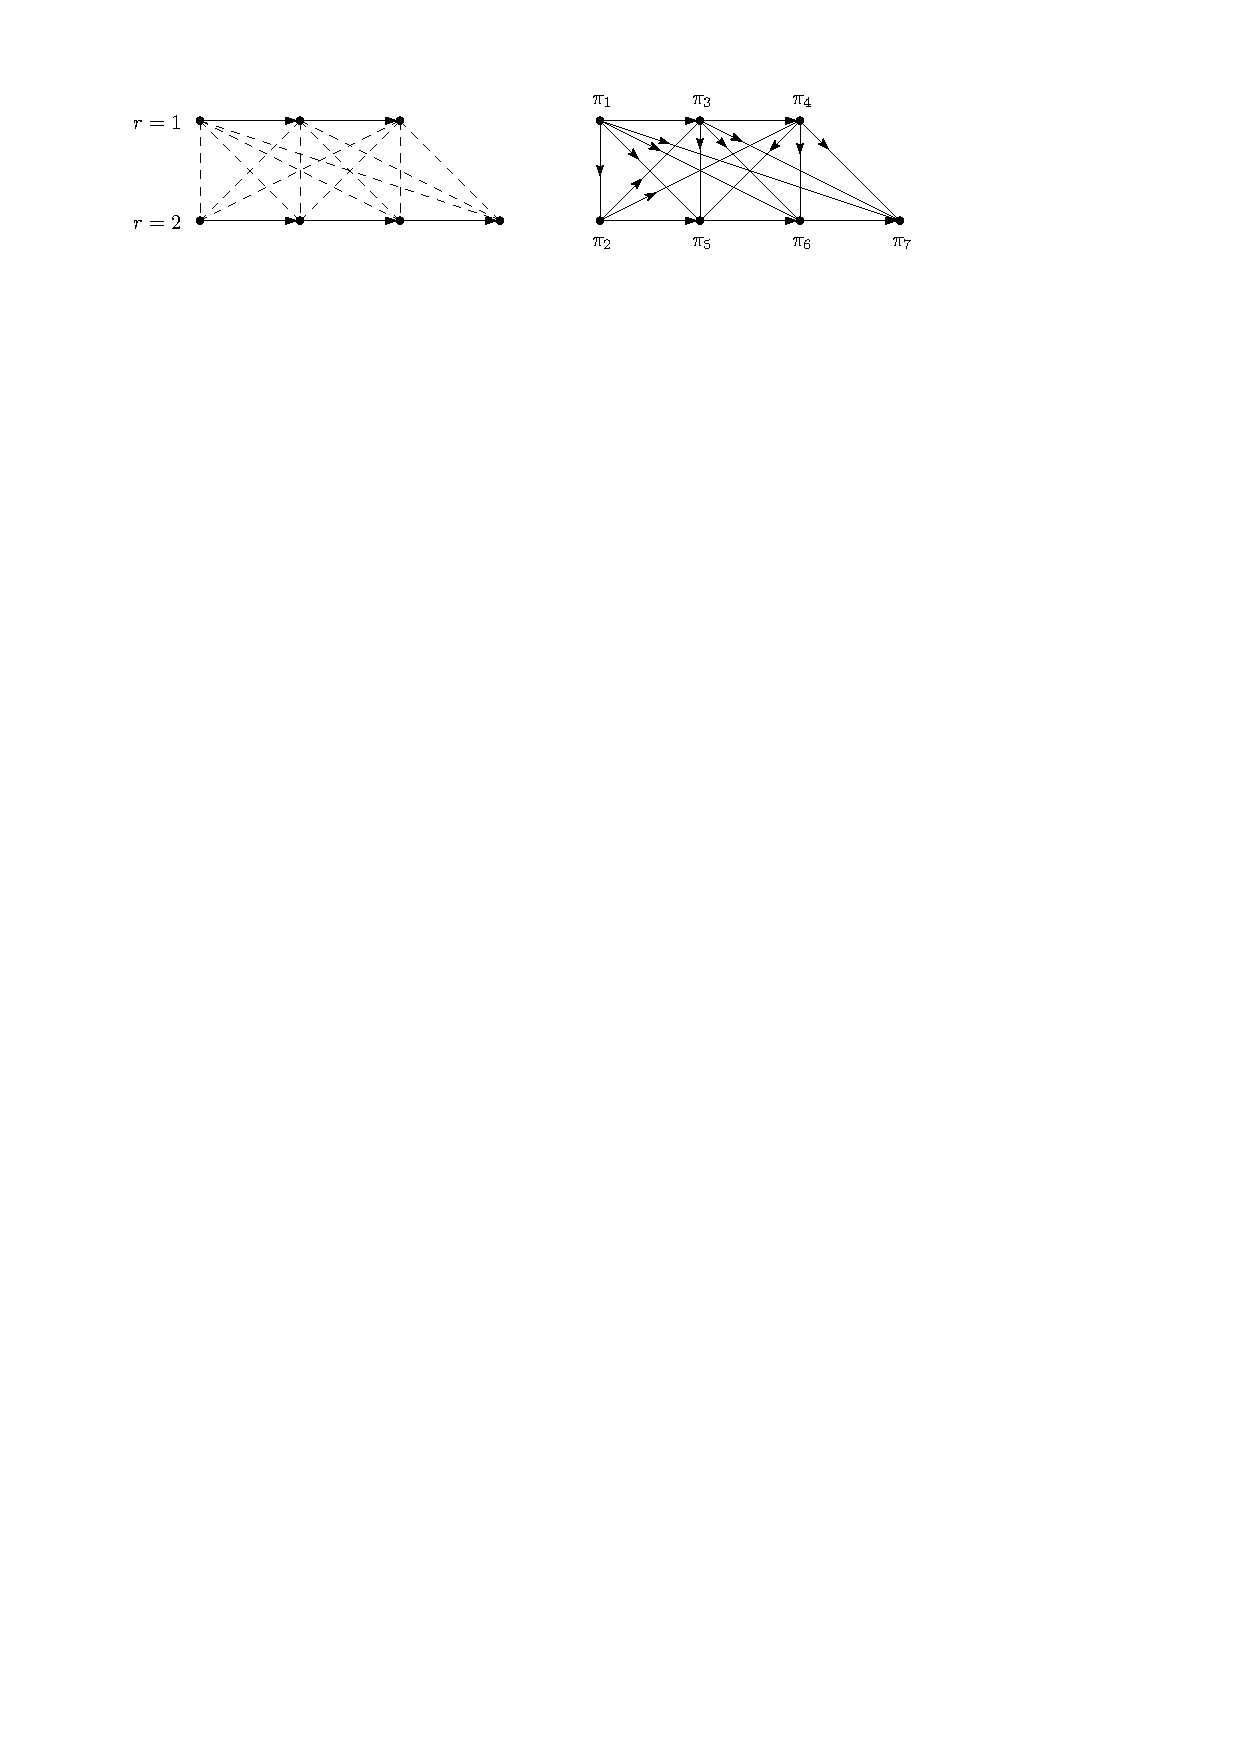
\includegraphics[width=0.98\textwidth]{figures/single/disjunctive_graph.pdf}
  \caption{Illustration of disjunctive graphs for some instance with two routes
    with $n_{1} = 3$ and $n_{2} = 4$ vehicles. Horizontal arrows are the
    conjunctive arcs, the rest are disjunctive arcs. The left graph is and
    \textit{empty} disjunctive graph, because $\mathcal{O} = \varnothing$. The
    selection of disjunctions shown in the \textit{complete} graph on the right
    encodes the vehicle order
    $\pi = ((1,1), (2,1), (1,2), (1,3), (2,2), (2,3), (2,4))$ and route order
    $\eta = (1, 2, 1, 1, 2, 2, 2)$.}
  \label{fig:disjunctive_graphs}
\end{figure}

\paragraph{Autoregressive modeling of schedules.}
Given some problem instance $s$, we now want to model the sequence $\eta$ such
that $y^{\eta}$ is an optimal schedule. To this end, we model the conditional
probability of $\eta$ given $s$ by considering autoregressive models of the form
\begin{align}
  \label{eq:autoregressive}
  p(\eta | s) = \prod_{t=1}^{N} p(\eta_{t} | s, \eta_{1:t-1}) ,
\end{align}
where $N$ denotes the total number of vehicles. Now consider some distribution
of problem instances $\mathcal{X}$, then our goal is to minimize the expected
value
\begin{align*}
  \mathbb{E}_{s \sim \mathcal{X}, \eta \sim p(\eta | s)} L(s, \eta) ,
\end{align*}
of the total vehicle delay
\begin{align*}
  L(s, \eta) = \sum_{i \in \mathcal{N}} y^{\eta}_{i} - a_{i} .
\end{align*}
%
For inference, we would ideally want to calculate the maximum likelihood
estimator
\begin{align*}
  \arg\max_{\eta} p(\eta | s) ,
\end{align*}
but this is generally very expensive to compute, because this could require
$O(|\mathcal{R}|^{N})$ evaluations of $p(\eta_{t} | s, \eta_{1:t-1})$ when we do
not make additional structural model assumption. Therefore, one often uses
\textit{greedy rollout}, which means that we pick $\eta_{t}$ with the highest
probability at every step.
% other inference methods
Other inference strategies have been proposed in the context of modeling
combinatorial optimization problems, see for example the ``Sampling'' and
``Active Search'' strategies in the seminal
paper~\cite{belloNeuralCombinatorialOptimization2017}.

% Instead of trying to map a problem instance directly to some optimal route
% order, we construct it in a step-by-step fashion. At every step, the partial
% route order induces a partial vehicle ordering, which is a permutation of the
% set of scheduled vehicles.
%
% It may be helpful to model this process as a finite-state automaton, where the
% set of route indices acts as the action space\footnote{We will later define a
%   reward, which turns the automaton into a deterministic Markov decision
%   process, so we find it more natural to say ``action space'' instead of the
%   common terminology ``input alphabet''.} $\mathcal{R} = \{ 1, \dots, n \}$. Let $S$
% denote the state space and let $\delta: S \times \mathcal{R} \rightarrow S$ denote the transition
% function.
% % states
% Let $s$ denote an instance of crossing time scheduling
% problem~\eqref{eq:crossing_time_scheduling}. We consider $s$ to be a fixed part
% of the state, so it does not change with transitions. The other part of the
% state is the current partial ordering $\pi_{t}$. The initial state is
% $s_{0} = (s, \varnothing)$.
% % transitions
% Let $s_{t} = (s, \pi) \in S$ denote some state and let $r \in \mathcal{R}$ be the next
% action that was chosen. Let $i$ denote the next unscheduled vehicle on route $r$,
% then the system transitions to $s_{t+1} = (s, \pi \mdoubleplus i)$, where
% $\mdoubleplus$ denotes sequence concatenation. If there was no next unscheduled
% vehicle $i$, the transition is undefined.
% %
% Suppose that we have some mapping $p : S \rightarrow \mathcal{R}$ to determine the next
% route, the final state can be determined by recursively computing
% \begin{align*}
%   s_{t} = \delta(s_{t-1}, p(s_{t-1})) .
% \end{align*}
%
% The goal is now to find a mapping $p$ such that the final state
% $s_{N} = (s, \pi^{*})$ correspond to some optimal ordering $\pi^{*}$.
%
% Observe that such a mapping must exist, because we can always set
% $p(s_{t}) = \eta^{*}_{t+1}$ for every step $t$, given some optimal route order
% $\eta^{*}$. However, we do not hope to find an explicit representation of $p$,
% because it would in general be very complex, so our aim is to find good
% approximations.

% multi-step transition
% With a little abuse of notation, let $\delta(s, \eta) = \delta(s_{0}, \eta)$ denote the
% state that we obtain after applying sequence $\eta$ to the automaton with initial
% state $s_{0} = (s, \varnothing)$, which generalizes the single step transition function by
% recursively defining
% \begin{align*}
%   \delta(s_{0}, \eta_{1:t}) = \delta(\delta(s_{0}, \eta_{1:t-1}), \eta_{t}) .
% \end{align*}
%
% Therefore, an input sequence $\eta$ of routes is called a \textit{valid route
%   order} whenever it is of length
% \begin{align*}
%   N = \sum_{r \in \mathcal{R}} n_{r}
% \end{align*}
% and contains precisely $n_r = |\{ i \in \mathcal{N} : r(i) = r \}|$ occurrences
% of route $r \in \mathcal{R}$.

\section{Model parameterization}

We can consider different ways of parameterizing $p(\eta | s)$ in terms of
$p(\eta_{t+1} | s, \eta_{1:t})$. Here, each partial sequence $\eta_{1:t}$
represents some partial schedule, which can equivalenty be defined in terms of
the sequence of \textit{scheduled} vehicles $\pi_{1:t}$. However, it is more
convenient to define a partial schedule in terms of the \textit{partial
  disjunctive graph} $G_{t} = (\mathcal{N}, \mathcal{C} \cup \mathcal{O}_{t})$,
which is defined by the unique selection $\mathcal{O}_{t}$ such that for each
$i \in \pi_{1:t}$ and each $\{i, j\} \in \mathcal{D}$, we have either
$(i, j) \in \mathcal{O}_{t}$ or $(j, i) \in \mathcal{O}_{t}$ with
$j \in \pi_{1:t}$.
%
To emphasize this parameterization in terms of the partial disjunctive graph, we
can alternatively write~\eqref{eq:autoregressive} as
\begin{align*}
  p(\eta | s) = \prod_{t=1}^{N} p(\eta_{t} | G_{t-1}) .
\end{align*}

There is a natural extensions of expression~\eqref{eq:y_max} for partial
disjunctive graphs. Given $G_{t}$, let the \textit{earliest crossing time} of
each vehicle $i \in \mathcal{N}$ be recursively defined as
\begin{align*}
  \beta_{t}(j) = \max\{ a_{j}, \max_{i \in \mathcal{N}^{-}_{t}(j)} \beta_{t}(i) + w(i,j) \} ,
\end{align*}
where $\mathcal{N}^{-}_{t}(j)$ denotes the set of in-neighbors of node $j$ in
$G_{t}$.
%
For empty schedules, we have $\beta_{0}(i) = a_{i}$ for all $i$. For complete
schedules, we have $\beta_{N}(i) = y^{\eta}(i)$ for all $i$. We have
$\beta_{t}(i) \leq \beta_{t+1}(i)$ for all $i$, because
$\mathcal{O}_{t} \subset \mathcal{O}_{t+1}$. Hence, $\beta_{t}$ can be
interpreted as providing the best lower bounds $\beta_{t}(i) \leq y^{\eta}(i)$,
regardless of how the partial schedule is completed.

\paragraph{Threshold heuristic.}

We know from Proposition~\ref{prop:exhaustive} that whenever it is possible to schedule a vehicle
immediately after its predecessor on the same route, then this must be done in
any optimal schedule.
%
Based on this idea, we might think that the same holds true whenever a vehicle
can be scheduled \textit{sufficiently} soon after its predecessor. Although this is not
true in general, we can define a simple heuristic based on this idea.

In this case, the model does not specify a distribution over $\eta$, but selects
a single candidate by selecting a single next route in each step, so with
$\mathds{1}\{ \cdot \}$ denoting the indicator function, we have
$p(\eta_{t+1} | G_{t}) = \mathds{1}\{ \eta_{t+1} = p_{\tau}(G_{t}) \}$,
selecting the next route at step $t$ as
% For every route $r \in \mathcal{R}$, let $k(r)$ denote the number of vehicles that
% have already been scheduled. Hence, let $i = (\eta_{t}, k(\eta_{t}))$ denote the
% vehicle that was scheduled in the last step.
\begin{align*}
  p_{\tau}(G_{t}) = \begin{cases}
                \eta_{t} \quad &\text{ if } \beta_{t}(\pi_{t}) + \rho + \tau \geq a_{j} \text{ and } (\pi_{t},j) \in \mathcal{C} , \\
                \texttt{next}(\eta_{t}) & \text{ otherwise, }
              \end{cases}
\end{align*}
where $\texttt{next}(\eta_{t})$ denotes some arbitrary route other than $\eta_{t}$ with
unscheduled vehicles left.
%
The threshold heuristic is illustrated in Figure~\ref{fig:threshold_heuristic}.

\begin{figure}
  \centering
  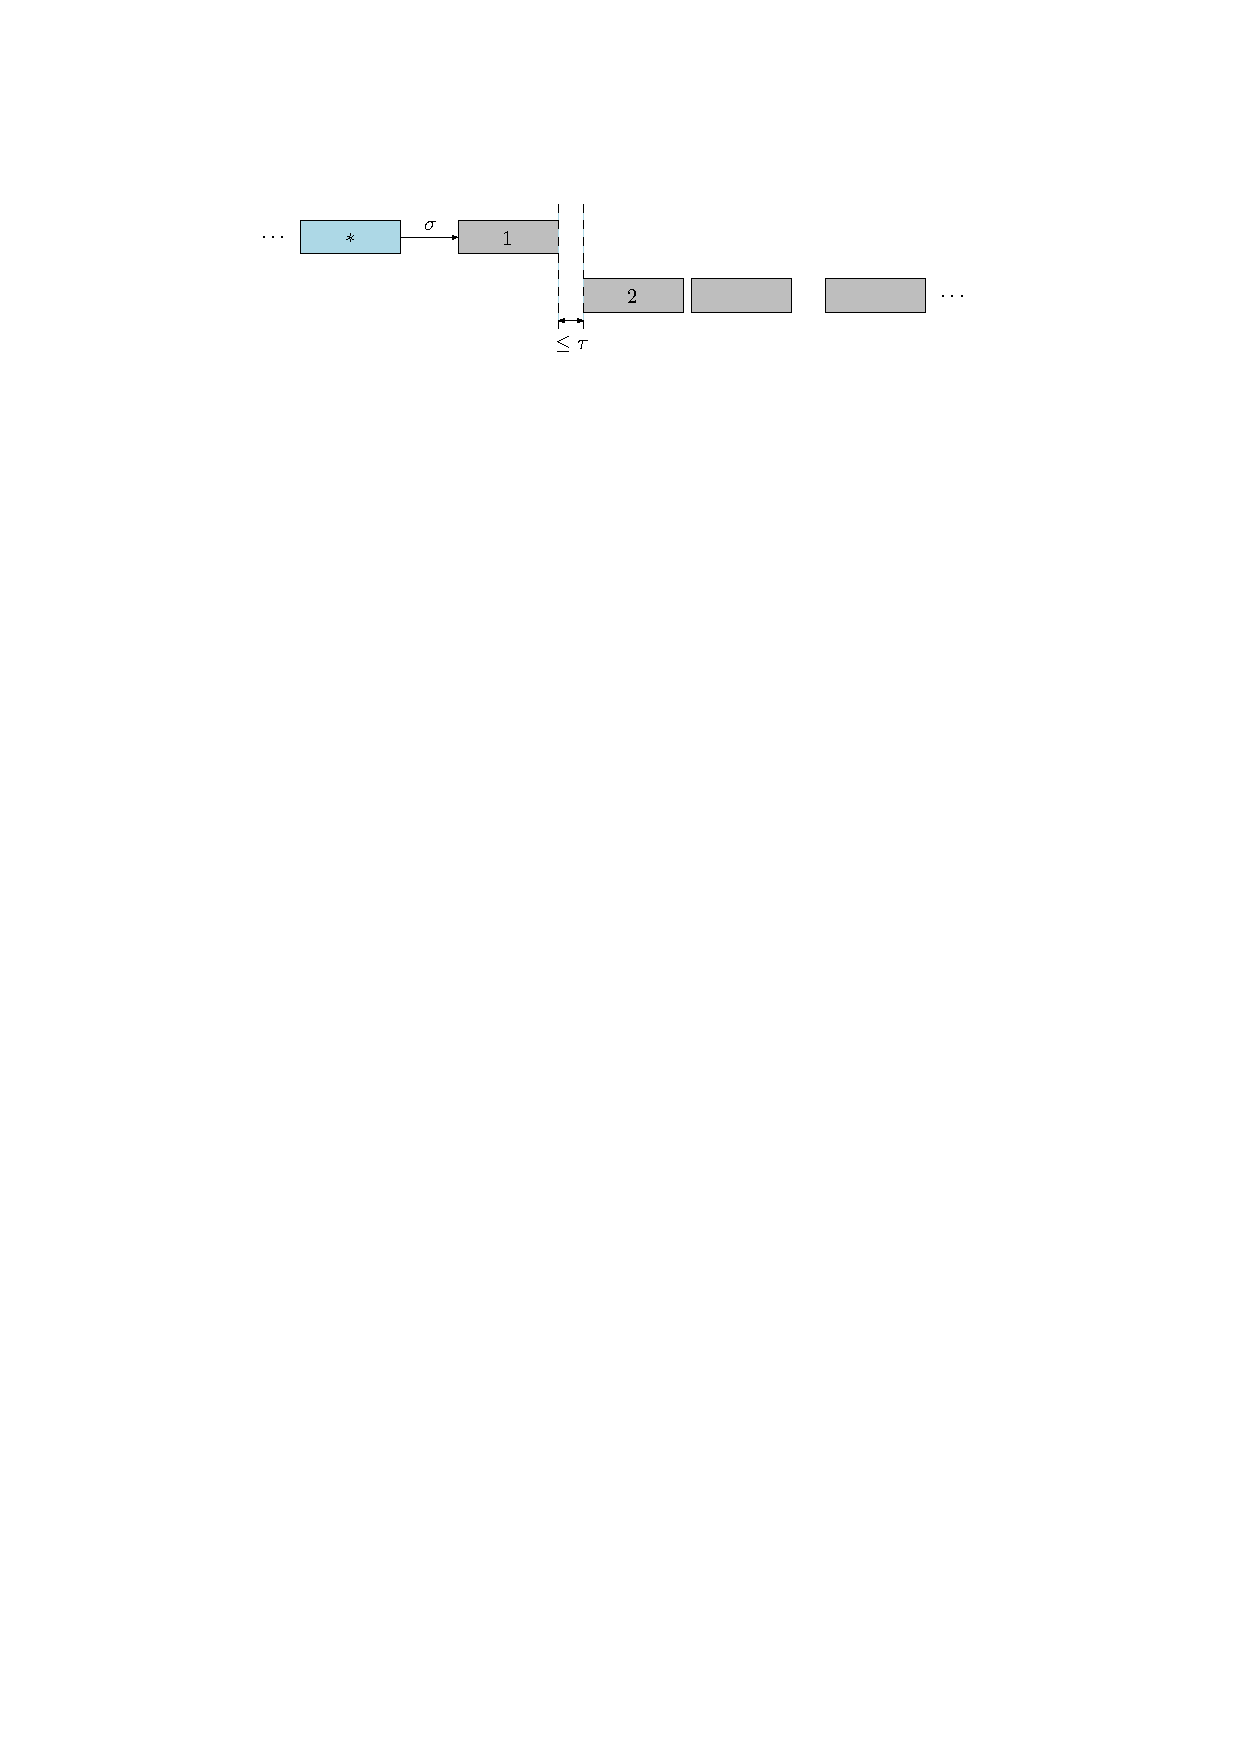
\includegraphics[width=0.8\textwidth]{figures/single/threshold}
  \caption{Illustration of how the threshold heuristic is evaluated at some
    intermediate step $t$ to choose the next route $\eta_{t+1}$. The top and
    bottom row contains the unscheduled vehicles from route 1 and route 2,
    respectively, drawn at their earliest crossing times $\beta_{t}(i)$. The
    middel row represents the current partial schedule. Vehicle $\pi_{t-1}$ is
    from route 1 and the last scheduled vehicle $\pi_{t}$ is from route 2 and
    the disjunctive constraint for them happens to be tight in this case,
    illustrated by the arrow. Whenever the indicated distance is smaller than
    $\tau$, the threshold rule selects vehicle $*$ to be scheduled next. Otherwise,
    vehicle $\dagger$ will be chosen.}\label{fig:threshold_heuristic}
\end{figure}


\paragraph{Neural parameterization.}

We will now consider a parameterizaton that directly generalizes the
threshold heuristic. Instead of looking at the earliest crossing time of the
next vehicle in the current lane, we now consider the earliest crossing
times of all unscheduled vehicles across lanes.
%
In the following definitions, we will drop the step index $t$ to avoid
cluttering the notation.
%
For every route $r$, let $\pi^{r}$ denote the sequence of unscheduled vehicles
and consider their crossing time lower bounds
$\beta(\pi^{r}) = (\beta(\pi^{r}_{1}), \beta(\pi^{r}_{2}), \dots)$. Let the
minimum crossing time lower bound among unscheduled vehicles be denoted by $T$,
then we call
$h_{r} = \beta(\pi^{r}) - T = (\beta(\pi^{r}_{1}) - T, \beta(\pi^{r}) - T, \dots)$
the \textit{horizon} of route $r$.

Next, we define some neural embedding $\bar{h}_{r}$ of each horizon. Observe
that horizons can be variable length. We could fix the length by using padding,
but this can be problematic for states that are almost done. Therefore, we
employ a recurrent neural network. Each horizon $h_r$ is simply transformed into
a fixed-length embedding by feeding it in reverse order through a plain Elman
RNN. Generally speaking, the most recent inputs tend to have greater influence
on the output of an RNN, which is why we feed the horizon in reverse order, such
that those vehicles that are due first are processed last, since we expect those
should have the most influence on the decision. These horizon embeddings are
arranged into a vector $h_{t}$ by the following cycling rule. At position $k$ of
vector $h_{t}$, we put the embedding for route
\begin{align*}
  k - \eta_{t} \; \mathrm{mod} \; |\mathcal{R}|
\end{align*}
where $\eta_{t}$ denotes the last selected route. Using this cycling, we make sure
that the embedding of the last selected route is always kept at the same
position of the vector.
% \begin{align*}
%   {H}_{r} = \bar{h}(r - \eta_{t} \; \mathrm{mod} \; |\mathcal{R}|) ,
% \end{align*}
%
Using some fully connected neural network $f_{\theta}$ and a softmax layer, this
global embedding is then finally mapped to a probability distribution as
\begin{align*}
  p_{\theta}(\eta_{t+1} | G_{t}) = \text{softmax} ( f_{\theta}(h_{t})) ,
\end{align*}
where $\theta$ denotes the parameters of $f$ and of the recurrent neural
networks.
% inference
After $\theta$ has been determined, we can apply greedy rollout by simply
ignoring routes that have no unscheduled vehicles left and take the argmax of
the remaining probabilities.

\begin{figure}
  \centering
  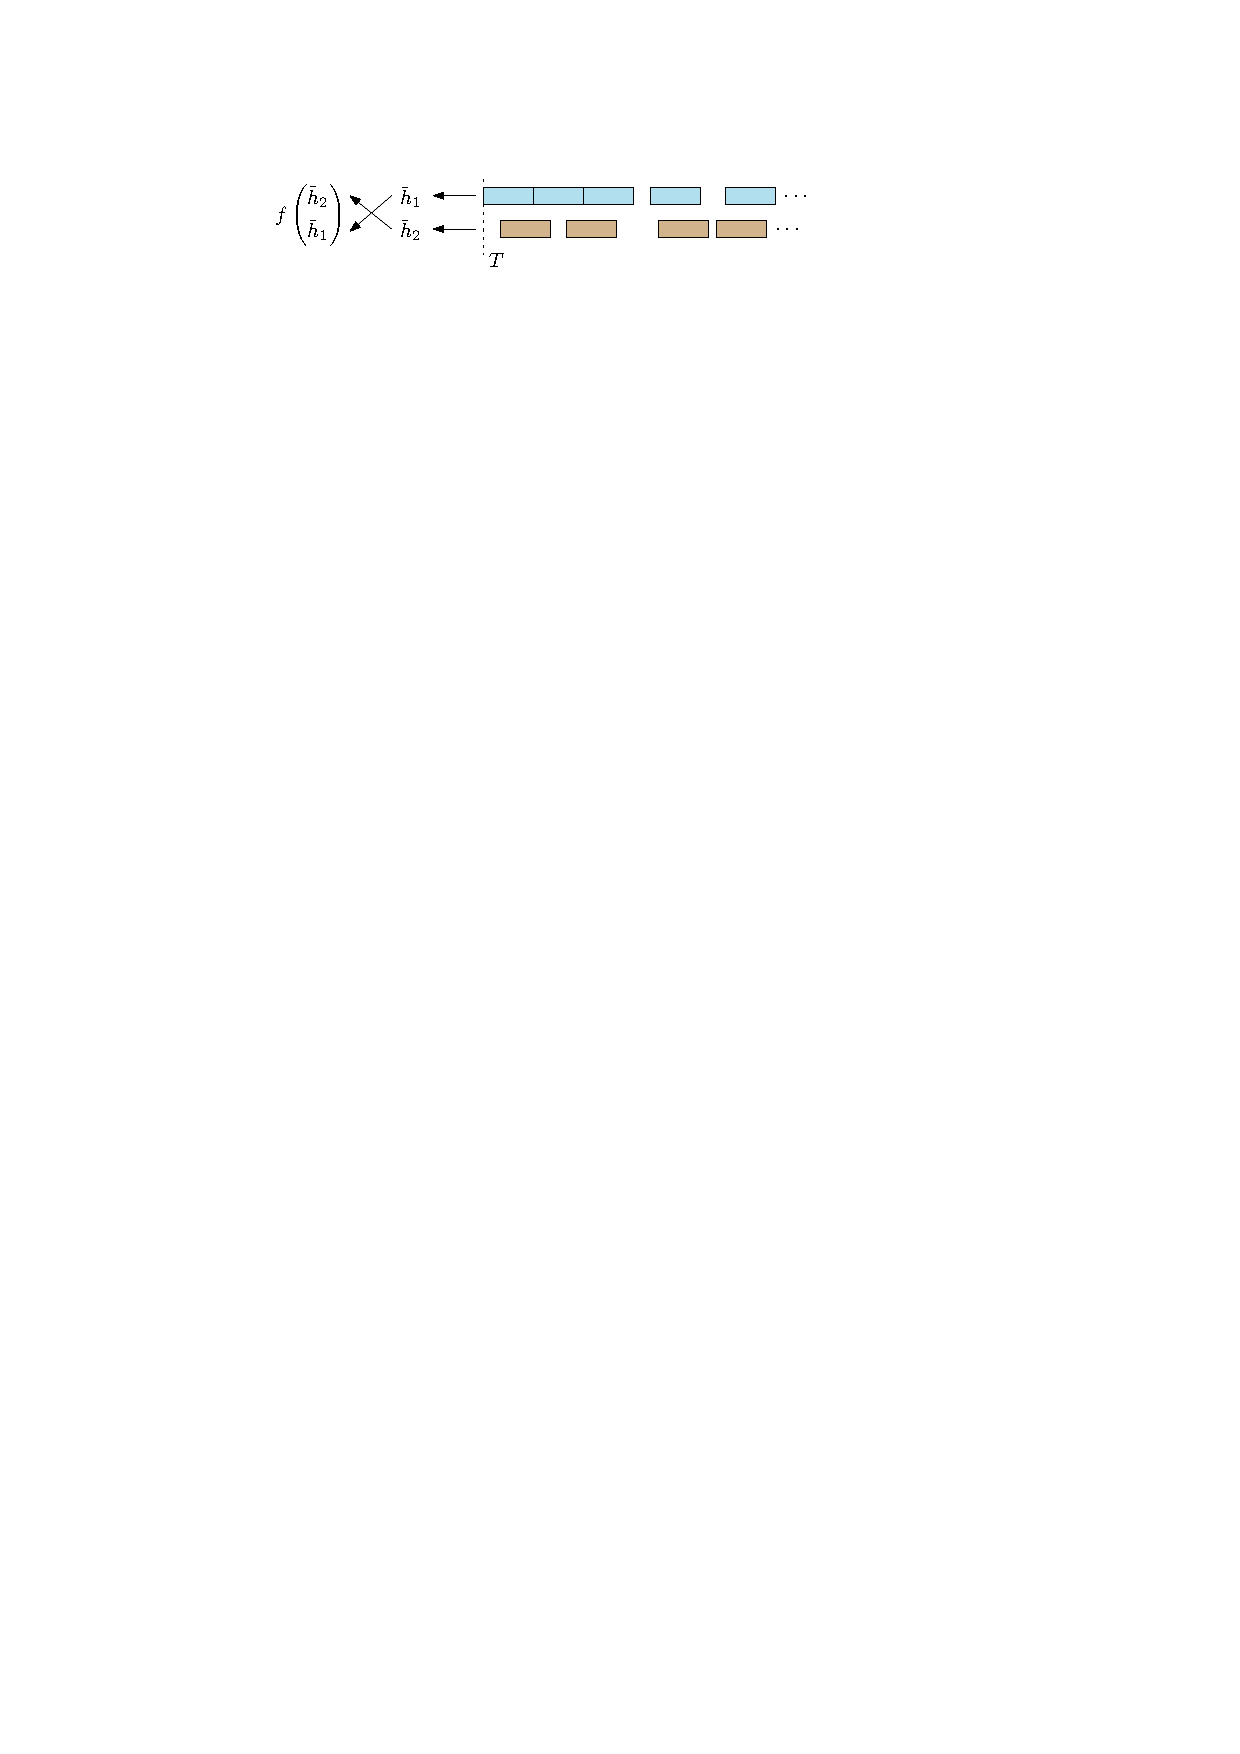
\includegraphics[width=0.8\textwidth]{figures/single/embedding}
  \caption{Schematic overview of parameterization of the neural heuristic. The
    distribution over the next route is parameterized as
    $p_{\theta}(\eta_{t+1} | G_{t})$, which is computed from the current route horizons
    $h_{r}$ via embeddings $\bar{h}_{r}$ and the cyling trick. Observe that the
    particular cycling shown in the figure corresponds to a situation in which
    the current route is $\eta_{t} = 2$.}\label{fig:neural_embedding}
\end{figure}


\section{Supervised learning}

We will now explain how model parameters can be tuned using some sample of
problem instances $X \sim \mathcal{X}$.
%
Given some instance $s$, let $\eta_{\tau}(s)$ be the schedule produced by the
threshold heuristic. Note that $L(s, \eta^{\tau}(s))$ is not differentiable with
respect to $\tau$, so we cannot use gradient-based optimization methods.
However, we only have a single parameter, so we can simply select the value of
$\tau$ that minimizes the average empirical loss
%
\begin{align*}
  \min_{\tau \geq 0} \sum_{s \in X} L(s, \eta_{\tau}(s)) ,
\end{align*}
%
which can be computed through a simple grid search.
%
This approach is no longer possible when $p(\eta \, | s)$ is a proper distribution,
so we need to something different for the neural parameterization.

Consider some instance $s \in X$ and let $\eta^{*}$ denote some optimal route
sequence, which can for example be computed by solving the MILP from
Section~\ref{sec:branch-and-cut}. For each such optimal schedule, we can compute
the sequence $G_{0}, \eta_{1}, G_{1}, \eta_{2}, \dots, \eta_{N}, G_{N}$. The
resulting set of pairs $\{ (G_{t}, \eta_{t+1}) : t = 1, \dots, N - 1 \}$ can be used to
learn $p_{\theta}$ in a supervised fashion by treating it as a classification task
and computing the maximum likelihood estimator $\hat{\theta}$. Interpreting $G_{t}$
as \textit{states} and $\eta_{t+1}$ as \textit{actions}, we see that this
approach is equivalent to \textit{imitation learning} in the context of finding
policies for Markov decision processes from so-called \textit{expert
  demonstration}.
%
Let $Z$ denote the set of all state-action pairs collected from all
training instances $X$. We make the procedure concrete for the case of two
routes $\mathcal{R} = \{ 1, 2 \}$, which is slightly simpler. Let $p_{\theta}(G_{t})$
denote the probability of choosing the first route, then we can use the binary
cross entropy loss, given by
\begin{align*}
  L_{\theta}(Z) = - \frac{1}{|Z|} \sum_{(G_{t}, \eta_{t+1}) \in Z} \mathds{1}\{\eta_{t+1} = 1\} \log(p_{\theta}(G_{t})) + \mathds{1}\{\eta_{t+1} = 2\} \log(1 - p_{\theta}(G_{t})) ,
\end{align*}
where $\mathds{1}\{\cdot\}$ denotes the indicator function. Now we can simply rely on
some gradient-descent optimization procedure to minimize $L_{\theta}(Z)$ with
respect to $\theta$.

\section{Reinforcement learning}

% imitation learning -> RL (on/off-policy)
Instead of using state-action pairs as examples to fit the model in a supervised
fashion (imitation learning), we can also choose to use the reinforcement
learning paradigm, in which the data collection process is guided by some
policy.

% reward definition
The reinforcement learning approach depends on the definition of a reward. For
each step $G_{t-1} \xrightarrow{\eta_{t}} G_{t}$, we can define a corresponding
reward, effectively yielding a deterministic Markov decision process.
Specifically, we define the reward at step $t$ to be
\begin{align*}
  R_{t} = \sum_{i \in \mathcal{N}} \beta_{t-1}(i) - \beta_{t}(i) .
\end{align*}
Let the return at step $t$ be defined as
\begin{align*}
  \hat{R}_{t} = \sum_{k=t + 1}^{N} R_{k} .
\end{align*}
Hence, when the \textit{episode} is done after $N$ steps, the total episodic
reward is given by the telescoping sum
\begin{align*}
  \hat{R}_{0} = \sum_{t=1}^{N} R_{t} = \sum_{i \in \mathcal{N}} \beta_{0}(i) - \beta_{N}(i)  = \sum_{i \in \mathcal{N}} a_{i} - y_{i} = - L(s, \eta) ,
\end{align*}
Therefore, maximizing the episodic reward corresponds to minimizing the
scheduling objective, as desired.
%

% REINFORCE
Policy-based methods work with an explicit parameterization of the policy. The
model parameters are then tuned based on experience, often using some form of
(stochastic) gradient descent to optimize the expected total return.
%
Therefore, the gradient of the expected return
plays a central role. The
following identity is generally known as the Policy Gradient Theorem:
\begin{align*}
  \nabla \mathbb{E}_{p} \hat{R}_{0} &\propto \sum_{s} \mu_{p}(s) \sum_{a} q_{p}(s, a) \nabla p(a | s, \theta) \\
  &= \mathbb{E}_{p}\left[ \sum_{a} q_{p} (S_{t}, a) \nabla p (a | S_{t}) \right] \\
  &= \mathbb{E}_{p}\left[ \sum_{a} p(a | S_{t}) q_{p} (S_{t}, a) \frac{\nabla p (a | S_{t})}{p (a | S_{t})} \right] \\
  &= \mathbb{E}_{p}\left[ q_{p} (S_{t}, A_{t}) \frac{\nabla p (A_{t} | S_{t})}{p (A_{t} | S_{t})} \right] \\
  &= \mathbb{E}_{p} \left[ \hat{R}_{t} \log \nabla p (A_{t} | S_{t}) \right] .
\end{align*}
% \begin{align*}
%   \nabla \mathbb{E}_{a \sim p_{\theta}(a | s)} R(s, a) &= \nabla \sum_{a} p_{\theta}(a | s) R(s, a) \\
%   &= \sum_{a} \nabla p_{\theta}(a | s) R(s, a) \\
%   &= \sum_{a} p_{\theta}(a | s) \frac{\nabla p_{\theta}(a | s)}{p_{\theta}(a | s)} R(s, a) \\
%   &= \mathbb{E}_{a \sim p_{\theta}(a | s)} \left[  \frac{\nabla p_{\theta}(a | s)}{p_{\theta}(a | s)} R(s, a) \right] \\
%   &= \mathbb{E}_{a \sim p_{\theta}(a | s)} [ \nabla \log p_{\theta}(a | s) R(s, a) ] .
% \end{align*}
%
The well-known REINFORCE estimator is a direct application of the Policy
Gradient Theorem. At each step $t$, we update the parameters $\theta$ using a
gradient ascent update
\begin{align*}
  \theta \leftarrow \theta + \alpha \hat{R}_{t} \nabla \log p_{\theta}(\eta_{t} | G_{t}) ,
\end{align*}
with some fixed learning rate $\alpha$.
% add baseline to reduce variance
To reduce variance of the estimator, we can incorporate a so-called
\textit{baseline}, which is an estimate of the expected return of the current
state.
%
In the context of combinatorial optimization, the value of the baseline may be
interpreted as estimating the relative difficulty of an instance?

\section{Results}

The evalutation of model performance is roughly based on two aspects. Of course,
the quality of the produced solutions is important. Second, we need to take into
account the time that the algorithm requires to compute the solutions. We need
to be careful here, because we have both training time as well as inference
time for autoregressive models.
%
We study the effect of the problem instance distribution $\mathcal{X}$ by
varying the number of routes and number of arrivals per route, distribution of
interarrival times, arrival intensity per route and degree of platooning.

Let $N(s)$ denotes the total number of vehicles in instance $s$. To enable a
fair comparison across instances of various sizes, we report the quality of a
solution in terms of the average delay per vehicle $L(\eta, s) / N(s)$.
%
Given some problem instance $s$, let $\eta^{*}$ denote the schedule computed using
branch-and-bound. We use a fixed time limit of 60 seconds per instance for the
branch-and-bound procedure, in order to bound the total analysis time.
Therefore, it might be that $\eta^{*}$ is not really optimal for some of the larger
instances. Given some, possibly suboptimal, schedule $\eta$, we define its \textit{optimality gap}
as
\begin{align*}
  L(s, \eta) / L(s, \eta^{*}) - 1 .
\end{align*}
For each heuristic, we report the average optimality gap over all test
instances.

The performance of the threshold heuristic is evaluated based on optimal
solutions obtained using MILP in Table~\ref{tab:results1}.
%
With the specific choice $\tau = 0$, the threshold rule is related to the
so-called \textit{exhaustive policy} for polling systems, which is why we
consider this case separately. We plot the average objective for the values of
$\tau$ in the grid search, see Figure~\ref{fig:tau_fit}.

The neural heuristics is trained for a fixed number of training steps. At
regular intervals, we compute the average validation loss and store the current
model parameters. At the end of the training, we pick the model parameters with
the smallest validation loss. The results are listed in Table~\ref{tab:results2}.
%
For the neural heuristic with supervised (imitation) learning, we plot the
training and validation loss, see Figure~\ref{fig:neural_fit}. It can be seen that the model
converges very steadily in all cases.
%
For the policy gradient method using REINFORCE with baseline, the training loss
with episodic baseline is shown in Figure~\ref{fig:rl_neural_episodic_fit} and
for the stepwise baseline in Figure~\ref{fig:rl_neural_stepwise_fit}.

% silent package loading


\begin{knitrout}
\definecolor{shadecolor}{rgb}{0.969, 0.969, 0.969}\color{fgcolor}\begin{table}
\centering
\caption{\label{tab:results1}Performance evaluation of the branch-and-cut (MILP) approach and the threshold heuristic for different classes of instances with two routes. The first two columns specify the instance class based on the number of vehicles $n$ per route and the type of arrival distribution for each route. These arrival distributions are chosen such that the arrival intensity is the same, only the degree of platooning varies. Performance is measured in terms of $L(s, \eta) / N(s)$, averaged over 100 test instances. The optimality gap is shown in parentheses for the heuristics.
The threshold heuristic is fitted based on 100 training instances and the optimal threshold and training time is indicated. For branch-and-cut the average inference time is indicated. Note that we used a time limit of 60 seconds for all the branch-and-cut computations.}
\centering
\resizebox{\ifdim\width>\linewidth\linewidth\else\width\fi}{!}{
\begin{tabular}[t]{cc|rr|r|rrcc|rr|r|rrcc|rr|r|rrcc|rr|r|rrcc|rr|r|rrcc|rr|r|rrcc|rr|r|rrcc|rr|r|rr}
\toprule
n & type & MILP & time & exhaustive (gap) & threshold (gap) & $\tau_\text{opt}$ & time\\
\midrule
10 & low & 5.29 & 0.05 & 9.49 (79.45\%) & 7.78 (47.08\%) & 0.95 & 3.79\\
30 & low & 8.60 & 2.01 & 12.72 (47.88\%) & 11.31 (31.49\%) & 2.65 & 21.04\\
50 & low & 11.03 & 13.78 & 16.56 (50.20\%) & 14.60 (32.41\%) & 1.95 & 51.09\\
10 & med & 4.46 & 0.06 & 7.20 (61.32\%) & 6.39 (43.15\%) & 2.50 & 3.79\\
30 & med & 6.99 & 1.88 & 9.43 (34.97\%) & 8.96 (28.29\%) & 1.10 & 21.14\\
50 & med & 8.55 & 15.11 & 11.50 (34.40\%) & 10.77 (25.93\%) & 1.70 & 51.23\\
10 & high & 4.47 & 0.06 & 6.35 (42.04\%) & 5.70 (27.51\%) & 1.35 & 3.81\\
30 & high & 6.90 & 1.90 & 8.92 (29.19\%) & 8.58 (24.25\%) & 1.00 & 21.16\\
50 & high & 7.37 & 14.99 & 9.36 (26.94\%) & 8.88 (20.42\%) & 0.80 & 51.45\\
\bottomrule
\end{tabular}}
\end{table}

\end{knitrout}


% silent package loading


\begin{knitrout}
\definecolor{shadecolor}{rgb}{0.969, 0.969, 0.969}\color{fgcolor}\begin{table}
\centering
\caption{\label{tab:results2}Comparison of neural heuristics with supervised learning and reinforcement learning, based on average delay per vehicle for different classes of instances with two routes. The first two columns specify the instance class based on the number of vehicles $n$ per route and the type of arrival distribution for each route. These arrival distributions are chosen such that the arrival intensity is the same, only the degree of platooning varies. The supervised heuristic is fitted based on 100 train instances and results averaged over 100 test instances. We use two different ways to compute the baseline: single baseline per episode, or baseline for every step during the episode.}
\centering
\resizebox{\ifdim\width>\linewidth\linewidth\else\width\fi}{!}{
\begin{tabular}[t]{cc|rr|rr|rrcc|rr|rr|rrcc|rr|rr|rrcc|rr|rr|rrcc|rr|rr|rrcc|rr|rr|rrcc|rr|rr|rrcc|rr|rr|rr}
\toprule
n & type & supervised (gap) & time & episodic (gap) & time & stepwise (gap) & time\\
\midrule
10 & low & 5.34 (0.92\%) & 6.13 & 5.73 (8.27\%) & 92.42 & 5.54 (4.81\%) & 125.94\\
30 & low & 8.70 (1.15\%) & 9.90 & 9.81 (14.05\%) & 290.47 & 9.17 (6.67\%) & 782.60\\
50 & low & 11.15 (1.15\%) & 13.99 & 12.38 (12.32\%) & 517.16 & 12.13 (9.99\%) & 2423.15\\
10 & med & 4.53 (1.44\%) & 5.66 & 4.85 (8.65\%) & 94.26 & 4.66 (4.42\%) & 128.56\\
30 & med & 7.10 (1.62\%) & 9.75 & 8.34 (19.42\%) & 296.29 & 7.77 (11.22\%) & 789.75\\
50 & med & 8.66 (1.26\%) & 13.99 & 10.33 (20.80\%) & 518.25 & 10.10 (18.09\%) & 2434.19\\
10 & high & 4.54 (1.50\%) & 5.97 & 4.81 (7.49\%) & 94.93 & 4.56 (2.01\%) & 129.00\\
30 & high & 7.05 (2.13\%) & 9.85 & 7.88 (14.15\%) & 295.97 & 8.01 (16.07\%) & 791.48\\
50 & high & 7.52 (1.98\%) & 14.01 & 8.91 (20.86\%) & 518.51 & 8.41 (14.13\%) & 2437.07\\
\bottomrule
\end{tabular}}
\end{table}

\end{knitrout}




\microtypesetup{deactivate}
\part*{\hspace{-0.8em}\textsc{Part II}\\[0.6em] Network of Intersections\\[3em]
       \centering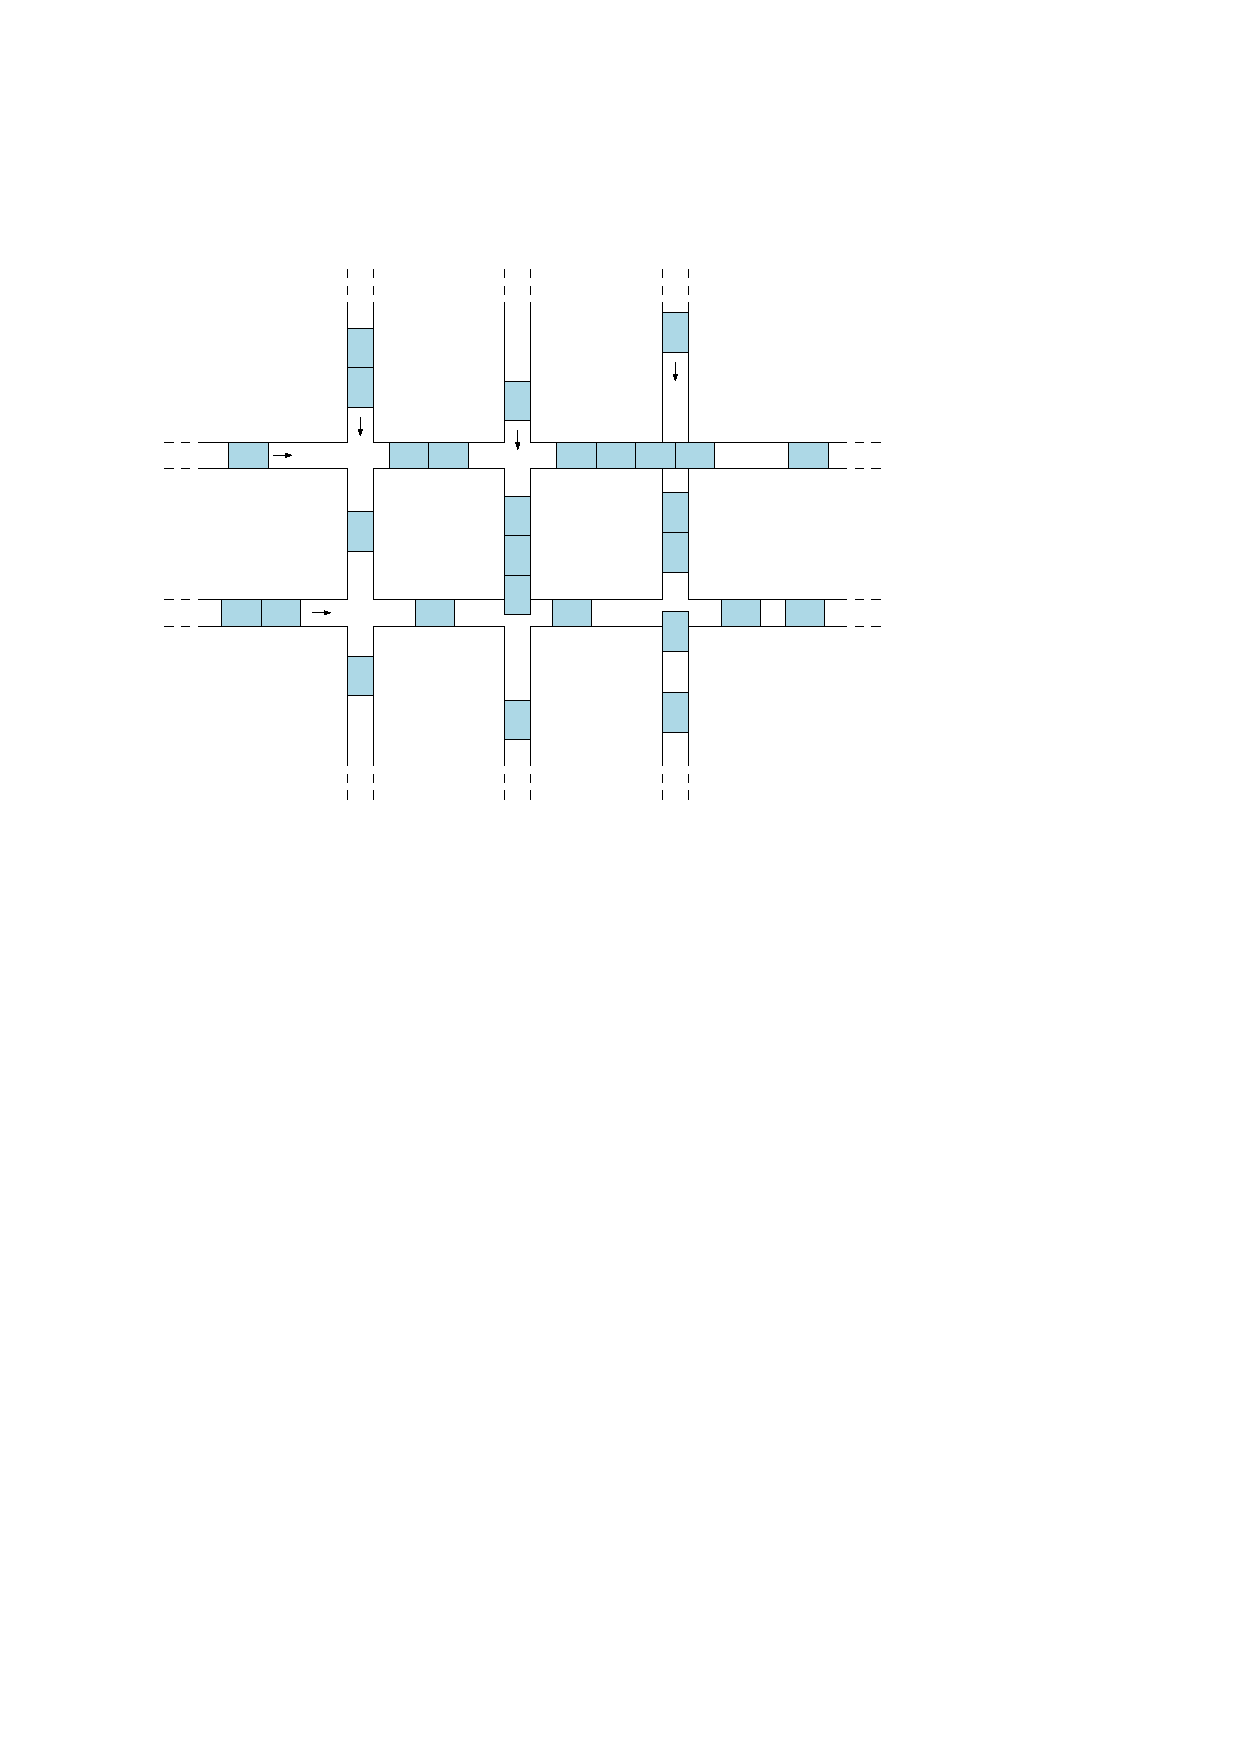
\includegraphics[scale=1]{figures/network-intersections}}
\microtypesetup{activate}
\addcontentsline{toc}{part}{Part II \;--\; Network of Intersections}

\chapter{Network with capacitated lanes}\label{chap:network}

There is a difference in how we will state the initial conditions of the system.
%
Recall that, in Chapter~\ref{chap:single}, we defined initial position
$x_{i}^{0}$ and velocity $v_{i}^{i}$ for each vehicle $i$.
This is also what is usually done when presenting an optimal control problem.
%
Instead, we will now consider the time of entry into the system.
%
These two notions are not necessarily equivalent.
%
Furthermore, we need to take special care in handling the domain of the
resulting trajectories, since they are now different for each vehicle.


\chapter{Learning to schedule}\label{chap:network-learning}

\addtocontents{toc}{\protect\renewcommand\cftbeforechapskip{2.5em}}
\chapter{Conclusion and discussion}\label{chap:conclusion}
\addtocontents{toc}{\protect\renewcommand\cftbeforechapskip{1em}}

% the code around the bibliographp itself serves as
% a sort of anchor for adding a bookmark entry
\phantomsection
\begin{singlespacing}\raggedright
\bibliographystyle{unsrt}
\bibliography{references}\label{sec:references}
\end{singlespacing}
% add entry to documents table of contents
\addcontentsline{toc}{chapter}{Bibliography}



\appendix

% add '.' after appendices in pdf bookmark, to avoid misreading 'A' as the first
% word of a sentence
\let\origthechapter\thechapter
\makeatletter
\xpatchcmd{\addcontentsline}{%
\Hy@writebookmark{\csname the#2\endcsname}%
      {#3}%
      {\@currentHref}%
      {\Hy@toclevel}%
      {#1}%
}{%
\begingroup
\renewcommand{\thechapter}{\origthechapter.}
\Hy@writebookmark{\csname the#2\endcsname}%
{#3}%
{\@currentHref}%
{\Hy@toclevel}%
{#1}%
\endgroup
}{\typeout{Success}}{}
\makeatother


\part*{Appendix}
\addcontentsline{toc}{part}{Appendix}

\chapter{Feasible configurations for single intersection
  model}\label{app:configuration-space}

\begin{figure}
  \centering
  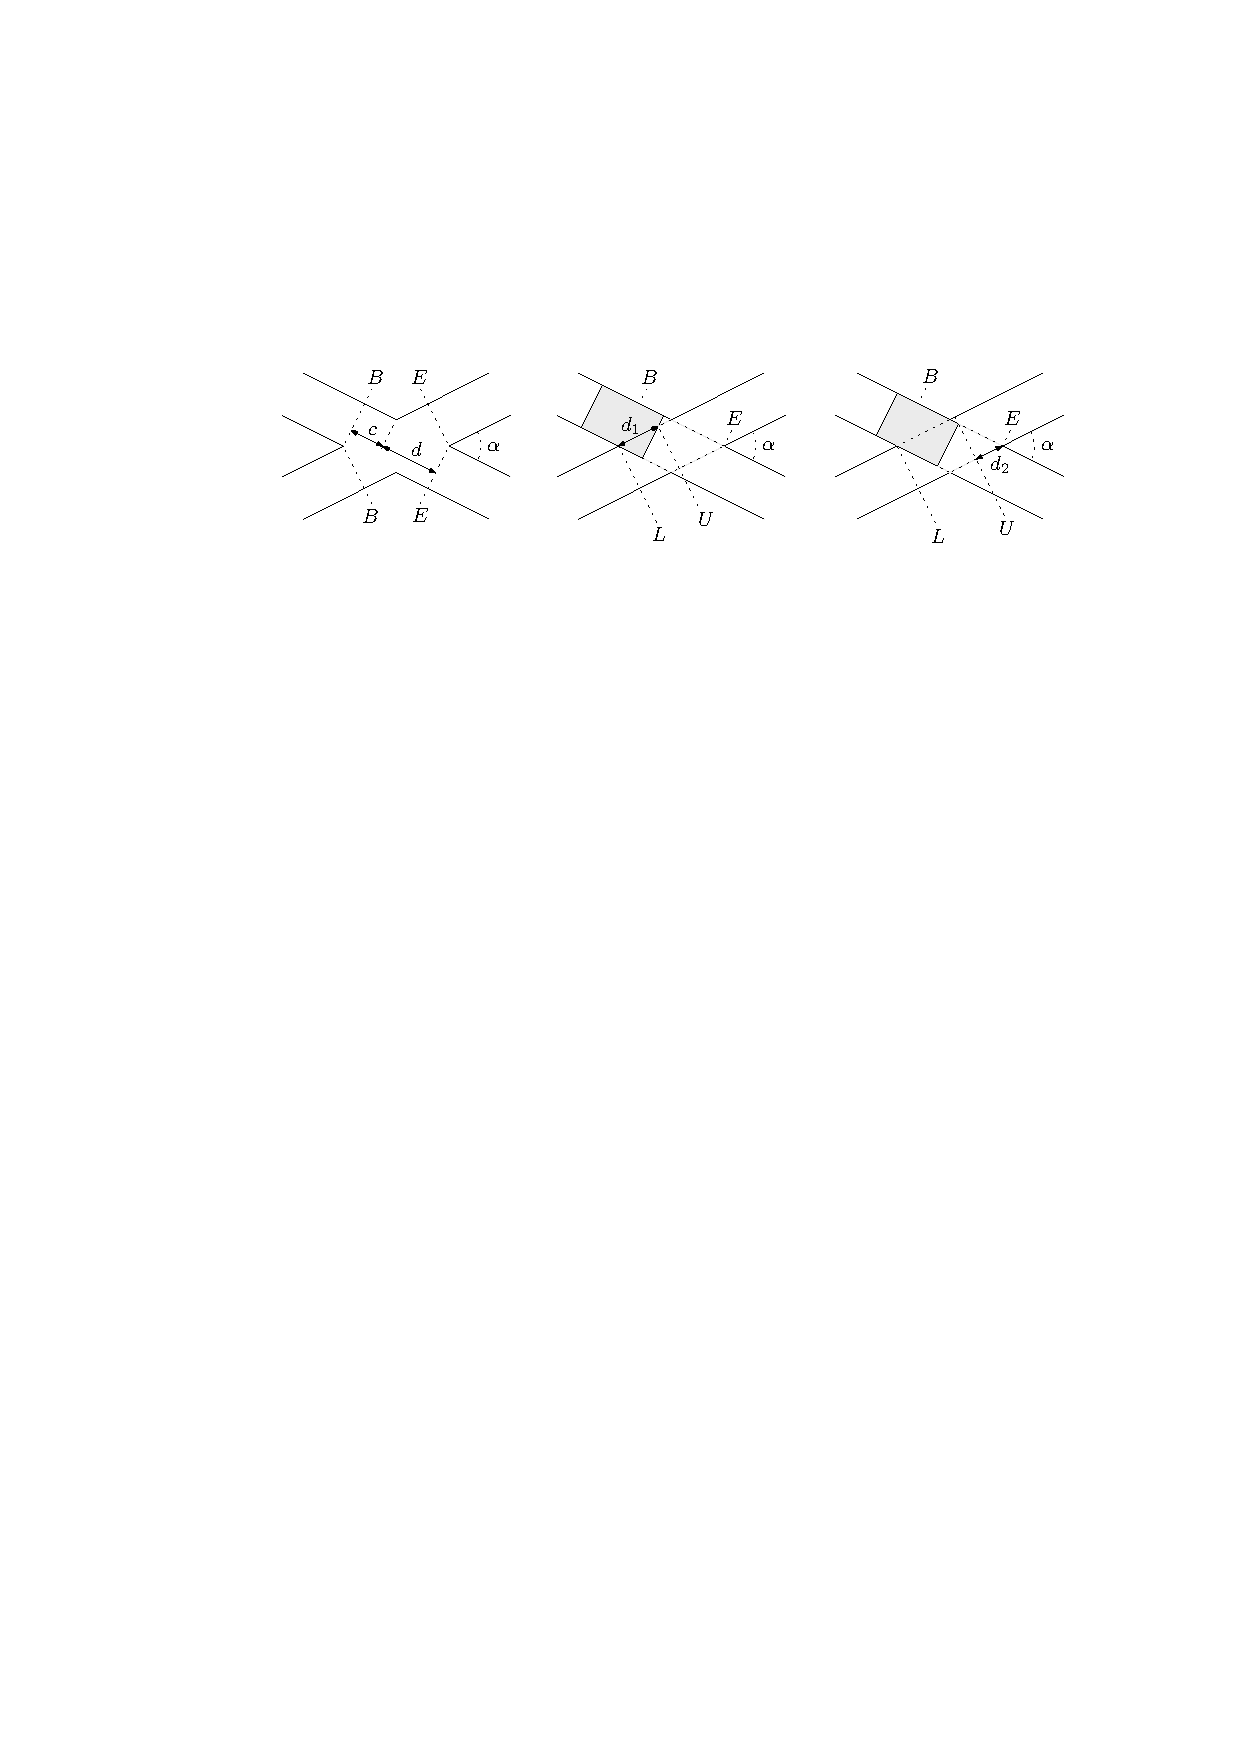
\includegraphics[scale=1]{figures/configuration-space}
  \caption{Sketches to derive the feasible configurations of two vehicles in the
    intersecting routes model. Using some elementary trigonometry, the distances
    in the first figure can be shown to be $c = W / \tan(\alpha)$ and
    $d = W / \sin(\alpha)$. Furthermore, observe that we have
    $(x_{i} - B) / d_{1} = \cos(\alpha)$ for
    $x_{i} \in \openhalf{B}{B + c}$, as shown in the middle figures and
    $d_{2}/(E - x_{i}) = \cos(\alpha)$ for $x_{i} \in \halfopen{B + c}{E}$,
    as shown in the right figure. These two types of distances can be used to
    derive the full characterization.}
  \label{fig:configuration-space}
\end{figure}

We present a way to derive the feasible configurations of the two routes that
intersect at some arbitrary angle, as shown in Figure~\ref{fig:intersection-non-axis-aligned}.
% general case
Assume that $\alpha < \pi / 2$ is the acute angle between the two intersections.
%
Furthermore, we consider uniform rectangular vehicle geometries with
$L_{i} \equiv L$ and $W_{i} \equiv W$, but the analysis is easily extended to
arbitrary dimensions.
%
We skip a thorough derivation of the following expressions, but we note that it
is based on the type of the distances illustrated in
Figure~\ref{fig:configuration-space}.
%
Roughly speaking, we encode the part of the intersection that vehicle $i$
occupies in terms of the other vehicle's $x_{j}$ coordinates, by defining the
following upper and lower limit positions
\begin{align}
  u(x_{i}) &:=
  \begin{cases}
    -\infty & \hspace{1.9em} \text{ if } x_{i} \leq B \text{ or } x_{i} - L \geq E , \\
    B + (x_{i} - E) / \cos(\alpha) & \hspace{1.9em} \text{ if } x_{i} \in \openhalf{E}{E + c\,} , \\
    E + (x_{i} - E) \cdot \cos(\alpha) & \hspace{1.9em} \text{ if } x_{i} \in \halfopen{E + c}{E} , \\
    E & \hspace{1.9em} \text{ if } x_{i} \geq E \text{ and } x_{i} - L < E ,
  \end{cases} \\
  l(x_{i}) &:=
  \begin{cases}
    B & \text{ if } x_{i} - L \leq E \text{ and } x_{i} > E , \\
    B + (x_{i} - L - E) / \cos(\alpha)     & \text{ if } x_{i} - L \in \openhalf{E}{E - c\,} , \\
    E + (x_{i} - L - E) \cdot \cos(\alpha) & \text{ if } x_{i} - L \in \halfopen{E - c}{E} , \\
    \infty & \text{ if } x_{i} - L \geq E \text{ or } x_{i} \leq E .
  \end{cases}
\end{align}
With these definitions, in order for the intersection to be free for vehicle
$j$, position $x_{i}$ must satisfy either $x_{i} < l(x_{j})$ or
$x_{i} - L > u(x_{j})$ and $x_{j}$ must satisfy either $x_{j} < l(x_{i})$ or
$x_{j} - L > u(x_{i})$.
%
Hence, these two pairs of equations completely determine the set of feasible
configurations, which can now be written as
\begin{alignat}{3}
  \mathcal{X}_{ij} = \{ (x_{i}, x_{j}) \in \mathbb{R}^{j} :& \; &&[\,x_{i} - L,x_{i} &]& \cap [\,l(x_{j}), u(x_{j}) &&] = \varnothing \\
  \text{ and } & \, &&[\,x_{j} - L, x_{j} &]& \cap [\,l(x_{i}), u(x_{i}) &&] = \varnothing \} .
\end{alignat}
%
In case the routes intersect at a right angle $\alpha = \pi / 2$, the situation
is much simpler and the two limiting positions are simply given by
\begin{align}
  (l(x_{i}), u(x_{i})) =
  \begin{cases}
    (B,  E)    &\text{ if } (x_{i} - L, x_{i}) \cap (B, E) \neq \varnothing , \\
    (\infty, -\infty) &\text{ otherwise, }
  \end{cases}
\end{align}
such that the set of feasible configurations is simply given by
\begin{align}
  \mathcal{X}_{ij} = \mathbb{R}^{2} \setminus [B,E + L]^{2} .
\end{align}

\chapter{REINFORCE with baseline}

For some fixed policy $\pi$ and initial state distribution $h$, we consider the
underlying \textit{induced Markov chain} over states. Because we are working with finite
episodes, the induced state process is a Markov chain with absorbing states.
%
We want to analyze how often states are visited on average, over multiple episodes.
%
To better understand what \textit{on average} means here, imagine that we link
together separate episodes to create a regular Markov chain without absorbing
states, in the following way: from each final state, we introduce state
transitions to the initial states according to distribution $h$, see also
Figure~\ref{fig:episodic_MC}. Furthermore, we will write $S_{t}^{(i)}$ to denote
the state at step $t$ of episode $i$.

\begin{figure}[h]
  \centering
  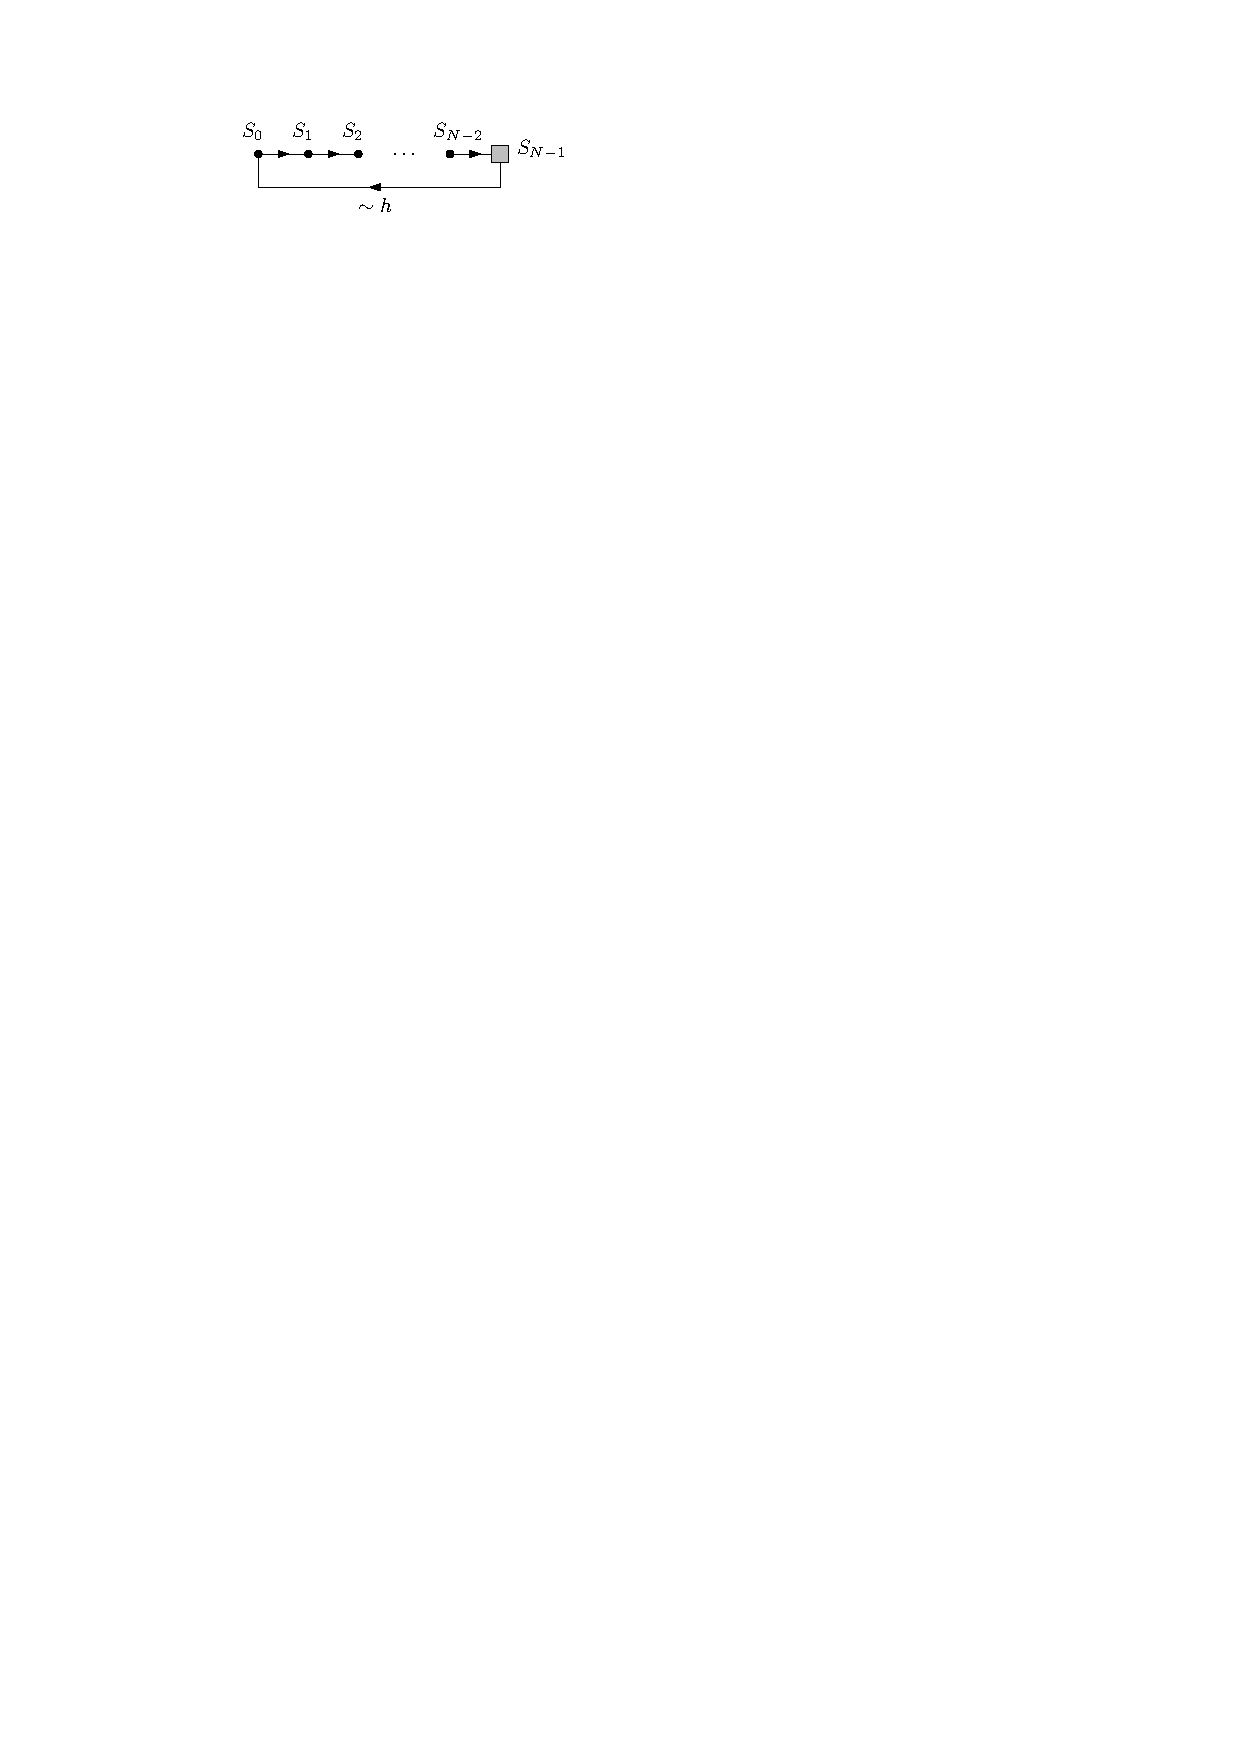
\includegraphics[width=0.4\textwidth]{figures/episodic_markov_chain.pdf}
  \caption{Illustration of the induced Markov chain when dealing with finite
    episodes. The next state after the final state, indicated as the grey
    rectangle, is sampled according to initial state distribution $h$.}
  \label{fig:episodic_MC}
\end{figure}


\section{Stationary distribution for finite episodes.}
Consider an absorbing Markov chain with transition matrix
\begin{align*}
  P_{xy} = \sum_{a} \pi(a | x) p(y | x, a) .
\end{align*}
There are $t$ transient states and $r$ absorbing states, so $P$ can be written
as
\begin{align*}
  P = \begin{pmatrix}
        Q & R \\
        \mathbf{0} & I_{r}
      \end{pmatrix} ,
\end{align*}
where $Q$ is a $t$-by-$t$ matrix, $R$ is a nonzero $t$-by-$r$ matrix, $I_{r}$ is
the $r$-by-$r$ identify matrix and $\mathbf{0}$ is the zero matrix.
%
Observe that $(Q^{k})_{xs}$ is the probability of reaching state $s$ in $k$
steps without being absorbed, starting from state $x$. Hence, the expected
number of visits to state $s$ without being absorbed, starting from state $x$,
is given by
\begin{align*}
  \eta(s | x) := \sum_{k=0}^{\infty} (Q^{k})_{xs} .
\end{align*}
%
Writing this in matrix form $N_{xs} = \eta(s | x)$, we can use the following
property of this so-called Neumann series, to obtain
\begin{align*}
  N = \sum_{k=0}^{\infty} Q^{k} = {(I_{t} - Q)}^{-1} .
\end{align*}
Now we can derive two equivalent equations
\begin{align*}
  N = (I_{t} - Q)^{-1} \iff
  \begin{cases}
    N (I_{t} - Q) = I_{t} \iff N = I_{t} + NQ ,
    \quad  \text{ or }  \\
    (I_{t} - Q) N = I_{t} \iff N = I_{t} + QN . \\
  \end{cases}
\end{align*}
%
Expanding the first equation in terms of matrix entries $N_{xs} = \eta(s | x)$
gives
\begin{align*}
  \eta(s | x) &= \mathds{1}\{ x = s \} + \sum_{y}  \eta(y | x) Q_{ys} \\
  &= \mathds{1}\{ x = s \} +  \sum_{y}\eta(y | x) \sum_{a} \pi(a | y) p(y | x, a)
\end{align*}
and similarly, the second equation gives
\begin{align*}
  \eta(s | x) &= \mathds{1}\{ x = s \} + \sum_{y} Q_{xy} \eta(s | y) \\
  &= \mathds{1}\{ x = s \} +  \sum_{a} \pi(a | x) \sum_{y} p(y | x, a) \eta(s | y)
\end{align*}
%
Now since the initial state is chosen according to distribution $h$, the
expected number of visits $\eta(s)$ to state $s$ in some episode is given by
\begin{align*}
  \eta(s) = \sum_{x} h(x) \eta(s | x) ,
\end{align*}
or written in matrix form $\eta = hN$, where $\eta$ and $h$ are row vectors.
%
Therefore, we can also work with the equations
\begin{align*}
  \begin{cases}
  hN = h + hNQ , \quad \text{ or } \\
  hN = h + hQN ,
  \end{cases}
\end{align*}
which are generally called \textit{balance equations}.
% or written in terms of matrix entries, respectively,
% \begin{align*}
%   \begin{cases}
%   \eta(s) = h(s) + \sum_{x} h(x) \sum_{y} \eta(y|x) \sum_{a} \pi(a|y)p(s|y, a) , \text{ or } \\
%   \eta(s) = h(s) + \sum_{x} h(x) \sum_{a} \pi(a | x) \sum_{y} p(y | x, a) \eta(s | y) .
%   \end{cases}
% \end{align*}
By writing the first variant as $\eta = h + \eta Q$ and expanding the matrix
multiplication, we obtain
\begin{align*}
  \eta(s) = h(s) + \sum_{y} \eta(y) \sum_{a} \pi(a|y)p(s|y,a) .
\end{align*}
%
Through appropriate normalization of the expected number of visits, we obtain
the average fraction of time spent in state $s$, given by
\begin{align*}
  \mu(s) = \frac{\eta(s)}{\sum_{s'} \eta(s')} .
\end{align*}

\paragraph{Monte Carlo sampling.}

Suppose we have some function $f : \mathcal{S} \rightarrow \mathbb{R}$ over
states and we are interested in estimating $\mathbb{E}_{S_{t}^{(i)} \sim \mu}[f(S_{t}^{(i)})]$.
%
We can just take random samples of $S_{t}^{(i)}$, by sampling initial state
$S_{0}^{(i)} \sim h$ and then \textit{rolling out} $\pi$ to obtain
\begin{align*}
\tau^{(i)} = (S_{0}^{(i)},A_{0}^{(i)},R_{1}^{(i)},S_{1}^{(i)},A_{1}^{(i)},R_{2}^{(i)},S_{2}^{(i)}, \dots, S_{N^{(i)}-1}^{(i)}) \sim \pi(\tau^{(i)} | S_{0}^{(i)}),
\end{align*}
where $N^{(i)}$ denotes the total number of states visited in this episode.
%
Given $M$ such episode samples, we compute the estimate as
\begin{align*}
  \mathbb{E}_{S_{t}^{(i)} \sim \mu} [ f(S_{t}^{(i)}) ] \approx \left( \sum_{i=1}^{M} \sum_{t=0}^{N^{(i)} - 1} f(S_{t}^{(i)}) \right) / \left( \sum_{i=1}^{M} N^{(i)} \right) .
\end{align*}

Observe that the analysis of the induced Markov chain can be extended to
explicitly include actions and rewards as part of the state and derive the
stationary distribution of the resulting Markov chain. However, we do not need
this distribution explicitly in practice, because we can again use episode
samples $\tau^{(i)}$. To keep notation concise, we will from now on denote this
type of expectation as $\mathbb{E}_{\tau \sim h,\pi}[f(\tau)]$ and omit episode
superscripts.
%
Using this new notation, note that the average episode length is given by
\begin{align*}
  \mathbb{E}_{h, \pi} [ N ]= \sum_{s'} \eta(s') .
\end{align*}

\section{Policy gradient estimation}

Let $v_{\pi_{\theta}} = \mathbb{E}_{h,\pi_{\theta}}[G_{0}]$ denote the expected
episodic reward under policy $\pi$, where $G_{t}$ is called the reward-to-go at
step $t$, which is defined as
\begin{align*}
  G_{t} := \sum_{k=t+1}^{\infty} R_{k} .
\end{align*}
The main idea of policy gradient methods is to update the policy parameters
$\theta$ in the direction that increases the expected episodic reward the most. This
means that the policy parameters are updated as
\begin{align*}
  \theta_{k+1} = \theta_{k} + \alpha \nabla v_{\pi_{\theta}} ,
\end{align*}
where $\alpha$ is the learning rate and the gradient is with respect to
$\theta$. Instead of trying to derive or compute the gradient exactly, we often
use some statistical estimate based on sampled episode. The basic policy
gradient algorithm is to repeat the three steps

\vspace{1em}
\noindent
\hspace*{1em} \texttt{1. sample $M$ episodes $\tau^{(1)}, \dots, \tau^{(M)}$ following $\pi_{\theta}$,}\\
\hspace*{1em} \texttt{2. compute gradient estimate $\widehat{\nabla v_{\pi_{\theta}}}(\tau^{(1)}, \dots, \tau^{(M)})$,} \\
\hspace*{1em} \texttt{3. update $\theta \leftarrow \theta + \alpha \widehat{\nabla v_{\pi_{\theta}}}$.}

\paragraph{REINFORCE estimator.}

We will now present the fundamental policy gradient theorem, which essentially
provides a function $f$ such that
\begin{align*}
  \nabla v_{\pi_{\theta}} = \mathbb{E}_{\tau \sim h,\pi_{\theta}}[f(\tau)] ,
\end{align*}
which allows us to estimate the policy gradient using episode samples.
%
To align with the notation
of~\cite{suttonReinforcementLearningIntroduction2018}, we write
$\mathrm{Pr}(x \rightarrow s, k, \pi) := (Q^{k})_{xs}$, for the probability of
reaching state $s$ in $k$ steps under policy $\pi$, starting from state some
$x$, so that the expected number of visits can also be written as
\begin{align*}
  \eta(s) = \sum_{x} h(x) \sum_{k=0}^{\infty} \mathrm{Pr}(x \rightarrow s, k, \pi)
\end{align*}
%
As proven in the chapter on policy gradient methods
in~\cite{suttonReinforcementLearningIntroduction2018}, the gradient of the value
function for a fixed initial state $s_0$ with respect to the parameters is given
by
\begin{align}
  \nabla v_{\pi}(s_{0}) = \sum_{s} \sum_{k=0}^{\infty} \mathrm{Pr}(s_{0} \rightarrow s, k, \pi) \sum_{a} q_{\pi}(s,a) \nabla \pi(a|s) .
\end{align}
When choosing the initial state $s_{0}$ according to some distribution
$h(s_{0})$, we verify that the final result is still the same as in
\cite{suttonReinforcementLearningIntroduction2018}:
\begin{subequations}
\begin{align}
  \nabla v_{\pi} :=& \nabla \mathbb{E}_{s_{0} \sim h}[v_{\pi}(s_{0})] \\
  =& \sum_{s_{0}} h(s_{0}) \sum_{s} \sum_{k=0}^{\infty} \mathrm{Pr}(s_{0} \rightarrow s, k, \pi) \sum_{a} q_{\pi}(s,a) \nabla \pi(a|s) \\
  =& \sum_{s} \eta(s) \sum_{a} q_{\pi}(s,a) \nabla \pi(a|s) \\
  =& \sum_{s'} \eta(s') \sum_{s} \mu(s) \sum_{a} q_{\pi}(s,a) \nabla \pi(a|s) \\
  \propto& \sum_{s} \mu(s) \sum_{a} q_{\pi}(s,a) \nabla \pi(a|s) ,
\end{align}
\end{subequations}
where the constant of proportionality is just the average episode length.
%
Because we do not know $\mu$ or $q_{\pi}$ explicitly, we would like to estimate
$\nabla v_{\pi}$ based on samples. If we sample episodes according to $h$ and
$\pi$ as explained above, we encounter states according to $\mu$, so we have
\begin{subequations}
\begin{align}
  \nabla v_{\pi} &\propto \mathbb{E}_{h, \pi} \left[ \sum_{a} q_{\pi}(S_{t}, a) \nabla\pi(a | S_{t}) \right] \\
  &= \mathbb{E}_{h, \pi} \left[ \sum_{a} \pi(a | S_{t}) q_{\pi}(S_{t}, a) \frac{\nabla \pi(a | S_{t})}{\pi(a | S_{t})} \right] \\
  &= \mathbb{E}_{h, \pi} \left[ q_{\pi}(S_{t}, A_{t}) \frac{\nabla \pi(A_{t} | S_{t})}{\pi(A_{t}| S_{t})} \right] \\
  &= \mathbb{E}_{h, \pi} \left[ G_{t} \nabla \log \pi(A_{t} | S_{t}) \right] .
  \label{eq:estimator1}
\end{align}
\end{subequations}

\paragraph{Baseline.}
Let $b(s)$ be some function of the state $s$ only, then we have for any $s \in \mathcal{S}$
\begin{align}
  \sum_{a} b(s) \nabla \pi(a | s) = b(s) \nabla \sum_{a} \pi(a | s) = b(s) \nabla 1 = 0 .
\end{align}
This yields the so-called REINFORCE estimate with \textit{baseline}
\begin{subequations}
\begin{align}
  \nabla v_{\pi} &\propto \sum_{s} \mu(s) \sum_{a} (q_{\pi}(s, a) + b(s)) \nabla \pi(a | s) \\
          &= \mathbb{E}_{h, \pi} \left[ \bigl(q_{\pi}(S_{t}, A_{t}) + b(S_{t}) \bigr) \nabla \log \pi(A_{t} | S_{t}) \right] \\
  &= \mathbb{E}_{h, \pi} \left[ \bigl(G_{t} + b(S_{t}) \bigr) \nabla \log \pi(A_{t} | S_{t}) \right] .
  \label{eq:estimator2}
          %&= \mathbb{E}_{h, \pi} \left[ \bigl(G_{t} + b(S_{t}) \bigr) \nabla \log \pi(A_{t} | S_{t}) \right]
\end{align}
\end{subequations}
%
Although estimates~\eqref{eq:estimator1} and~\eqref{eq:estimator2} are both equivalent in terms of their expected
value, they may differ in higher moments, which is why an appropriate choice of
$b$ can make a lot of difference in how well the policy gradient algorithm
converges to an optimal policy.
%
As a specific baseline, consider the expected cumulative sum of rewards up to
step the current step $t$, defined as
\begin{align}
  b(s) = \mathbb{E}_{h,\pi} \left[ \sum_{k=1}^{t} R_{k} \Big| S_{t} = s \right],
\end{align}
then observe that
\begin{subequations}
\begin{align}
  q_{\pi}(s, a) + b(s) &= \mathbb{E}_{h,\pi}\left[ \sum_{k=t+1}^{\infty} R_{k} \Big| S_{t} = s , A_{t} = a \right] + \mathbb{E}_{h,\pi}\left[ \sum_{k=1}^{t} R_{k} \Big| S_{t} = s \right] \\
                     &= \mathbb{E}_{h,\pi}\left[ \sum_{k=1}^{\infty}  R_{k} \Big| S_{t} = s, A_{t} = a \right] \\
                     &= \mathbb{E}_{h,\pi} [ G_{0} | S_{t} = s, A_{t} = a ] ,
\end{align}
\end{subequations}
which is just the expected total episodic reward.
%
Now define function $f$ to be
\begin{subequations}
\begin{align}
  f(s, a) := (q_{\pi}(s, a) + b(s))\nabla \log \pi(a | s) &= \mathbb{E}_{h,\pi} \left[ G_{0} | S_{t} = s, A_{t} = a \right] \nabla \log \pi(a | s) \\
  &= \mathbb{E}_{h,\pi} \left[ G_{0} \nabla \log \pi(a | s) | S_{t} = s, A_{t} = a \right] ,
\end{align}
\end{subequations}
then applying the law of total expectation yields
\begin{align}
  \nabla v_{\pi} \propto \mathbb{E}_{h,\pi}[f(S_{t}, A_{t})] =  \mathbb{E}_{h, \pi} \left[ G_{0} \nabla \log \pi(A_{t} | S_{t}) \right] .
\end{align}

\end{document}

% add extra flag when compiling from emacs
% Local Variables:
% TeX-command-extra-options: "-shell-escape"
% End:
